\RequirePackage[2023-11-01]{latexrelease}
\documentclass{rapportPFEHIND}

% ---- Packages supplémentaires (non chargés dans le .cls) ----
\usepackage{lipsum}
\usepackage{minted}
\usepackage{arabtex}
\usepackage{utf8}
\setcode{utf8}
\usepackage{array}
\usepackage{booktabs}
\usepackage{longtable}
\usepackage{wrapfig}
% NE PAS recharger xcolor ici — déjà dans le .cls
\usetikzlibrary{shapes,arrows,positioning}
\usepackage[export]{adjustbox}
\usepackage{tcolorbox}
\usepackage{amssymb}
\tcbuselibrary{most}
\usepackage{pdfpages}
\usepackage{placeins}
\usepackage{setspace}
\usepackage{emptypage}
\onehalfspacing
\raggedbottom

% ---- Couleurs personnalisées ----
\definecolor{bg}{rgb}{0.95,0.95,0.95}
\definecolor{tamtamblue}{RGB}{35,100,170}
\definecolor{sectioncolor}{RGB}{35,100,170}
\definecolor{subsectioncolor}{RGB}{70,130,180}
\definecolor{chapterblue}{RGB}{35,100,170}
\definecolor{lineblue}{RGB}{35,100,170}

% ---- Légendes des figures et tableaux ----
\captionsetup[figure]{font=small,labelfont=bf,textfont=bf,justification=centering}
\captionsetup[table]{font=small,labelfont=bf,justification=centering}
\setlength{\textfloatsep}{10pt plus 2pt minus 4pt}
\setlength{\floatsep}{10pt plus 2pt minus 4pt}
\setlength{\intextsep}{10pt plus 2pt minus 4pt}
\renewcommand{\topfraction}{0.9}
\renewcommand{\bottomfraction}{0.8}
\renewcommand{\textfraction}{0.07}
\renewcommand{\floatpagefraction}{0.8}

% ---- tocloft ----
\renewcommand{\cftfigfont}{\normalfont}
\renewcommand{\cftfigpagefont}{\normalfont}
\renewcommand{\listfigurename}{Liste des figures}
\renewcommand{\listtablename}{Liste des tableaux}
% Titres des listes en bleu
\renewcommand{\cftloftitlefont}{\Large\bfseries\color{sectioncolor}}
\renewcommand{\cftlottitlefont}{\Large\bfseries\color{sectioncolor}}
\renewcommand{\cfttoctitlefont}{\Large\bfseries\color{sectioncolor}}

% ---- Espacement des paragraphes ----
\setlength{\parskip}{6pt}

% ---- Configuration des titres ----
\titleformat{\section}
  {\fontsize{16}{19.2}\bfseries\color{sectioncolor}}
  {\thesection.}{0.5em}{}
\titlespacing*{\section}{0pt}{6pt}{6pt}

\titleformat{\subsection}
  {\fontsize{14}{16.8}\bfseries\color{subsectioncolor}}
  {\thesubsection}{0.5em}{}
\titlespacing*{\subsection}{0pt}{6pt}{6pt}

\titleformat{\subsubsection}
  {\fontsize{12}{14.4}\bfseries}
  {\thesubsubsection}{0.5em}{}
\titlespacing*{\subsubsection}{0pt}{6pt}{6pt}

\titleformat{\chapter}[display]
{\fontsize{16}{19.2}\bfseries\color{chapterblue}}
{\chaptertitlename\ \thechapter }
{20pt}
{\fontsize{18}{21.6}\color{chapterblue}}
[\vspace{10pt}{\color{lineblue}\rule{\textwidth}{2pt}}]

% ---- Commandes personnalisées ----
\newcommand{\chaptertoc}{%
    \vspace{1cm}
    \begin{tikzpicture}
        \node[anchor=west, font=\large\bfseries, color=chapterblue] at (0,1.5) {$\triangleright$ Étude fonctionnelle};
        \node[anchor=west, font=\large\bfseries, color=chapterblue] at (0,0.8) {$\triangleright$ Méthodologie de conception};
    \end{tikzpicture}
    \vspace{1cm}
    {\color{lineblue}\hrule height 2pt}
    \vspace{1cm}
}

\newcommand{\chapterintro}[1]{%
    \begin{flushleft}
    \textit{#1}
    \end{flushleft}
    \vspace{1cm}
}

\newcommand{\roundedimage}[2]{%
    \begin{tikzpicture}
        \node[inner sep=0pt] (image) {\includegraphics[width=#1]{#2}};
        \begin{scope}
            \clip[rounded corners=3mm] (image.south west) rectangle (image.north east);
            \node[inner sep=0pt] {\includegraphics[width=#1]{#2}};
        \end{scope}
    \end{tikzpicture}%
}

\title{Rapport de Projet de Fin d'Études}
\date{\today}

\begin{document}

% Page de garde — titlepage gère elle-même sa mise en page
\fairepagedegarde

% Page Bismillah — sans en-tête ni pied de page, sans numéro
\thispagestyle{empty}
\vspace*{2cm}
\begin{center}
%    
\includegraphics[width=\textwidth]{Meaning-of-bismillah-al-rahman-al-rahim.png}

\includegraphics[width=\textwidth]{basmala.png}
\end{center}
% \rule{\textwidth}{0.5pt}
\vspace{1cm}
{\centering
\LARGE
Bismillah is the key to all success,\\
A light before each word I confess.

Bismillah grants me strength and firmness,\\
Guiding my path with divine awareness.

Through faith and knowledge, I bear witness,\\
That Allah's name brings boundless blessedness.\\}

\clearpage

% Début numérotation romaine — pages liminaires
\pagenumbering{Roman}
\setcounter{page}{1}
\fairemarges

% Dédicaces — page I
\section*{Dédicaces}
Il est de la noblesse des gens de savoir rendre hommage à qui de droit. La grâce revient d'abord et avant tout à \textbf{Allah, le Tout-Puissant}, qui m'a accordé la patience, la force et la sagesse nécessaires pour mener à bien ce travail. Avant cela, Il m'avait déjà fait la grâce insigne de m'ouvrir les portes de l'ingénierie et de me guider vers des horizons que je n'aurais jamais imaginé atteindre.\\[6pt]
Ensuite, toute ma reconnaissance et ma gratitude vont à mes \textbf{chers parents bien-aimés} pour leurs sacrifices incommensurables, leurs efforts constants et leur dévouement sans limite depuis mon plus jeune âge. Cette dédicace leur est entièrement consacrée, eux qui sont la lumière de mon cœur, la source de mon éducation et les piliers de ma réussite. Voici que les fruits de leurs efforts et de leur patience commencent enfin à porter leurs résultats ; à eux, tout mon respect, ma gratitude éternelle et mon amour inconditionnel.\\[6pt]
À mes \textbf{frères et sœurs bien-aimés} : Zeinab, Asma et Anas, mes compagnons de vie, mes soutiens constants dans les moments difficiles et mes partenaires de joie dans les moments heureux.\\[6pt]
À mon \textbf{cher ami Yassine}, fidèle compagnon de route tout au long de ces années d'études, de persévérance et de croissance intellectuelle. Son amitié sincère et son soutien moral ont été des éléments précieux de mon parcours.\\[6pt]
Enfin, j'adresse cette dédicace à toutes les \textbf{victimes des conflits dans le monde}, aux orphelins et aux endeuillés qui portent le poids de la perte, ainsi qu'aux étudiants privés de leurs universités et de leur droit fondamental à l'éducation. Puisse chacun d'eux trouver son chemin vers un avenir meilleur, plus juste et empli d'espoir.
\vspace{2cm}
\clearpage

% Remerciements
\phantomsection
\addcontentsline{toc}{section}{Remerciements}
\section*{Remerciements}

Il m'est particulièrement agréable de m'acquitter d'une dette de reconnaissance auprès de toutes les personnes dont l'intervention bienveillante au cours de ce projet a favorisé son aboutissement dans les meilleures conditions possibles.

Mes sincères remerciements s'adressent en premier lieu au \textbf{Professeur Tarik Agouti}, mon encadrant pédagogique, pour son soutien constant, ses conseils judicieux et perspicaces, ainsi que son encadrement rigoureux et méthodique tout au long de ma période de stage. Sa disponibilité remarquable, son expertise technique et sa bienveillance pédagogique ont été déterminantes dans la réussite de ce projet.

Dans ce contexte, je remercie respectueusement \textbf{Monsieur Emmanuel DEGRÈVE}, directeur fondateur de l'entreprise TAMTAM International, pour m'avoir accordé sa confiance en m'acceptant comme stagiaire au sein de son entreprise innovante et dynamique. Son leadership visionnaire et sa philosophie d'entreprise ont créé un environnement propice à l'apprentissage et au développement professionnel.

Je tiens à exprimer ma profonde gratitude à l'entreprise \textbf{TAMTAM International} pour m'avoir offert cette opportunité de stage exceptionnellement enrichissante et formatrice. Mes remerciements particuliers vont à \textbf{Mme ELKHROF Leila} pour sa disponibilité remarquable, son écoute attentive et bienveillante, ainsi que son encadrement méticuleux et professionnel qui ont grandement favorisé ma progression technique et mon épanouissement professionnel.

Par ailleurs, j'adresse mes chaleureux remerciements à toute l'équipe TAMTAM International, et en particulier aux membres talentueux de l'équipe "oFFFCourse" : \textbf{Youssef ATTAR}, \textbf{Yassine MESTAOUI} et \textbf{Youness OULAMINE}, pour leur accueil bienveillant, leur professionnalisme exemplaire, leur collaboration fructueuse et leur aide précieuse pendant cette période de formation intensive.
J'exprime également ma profonde gratitude et mes vifs remerciements à tous les membres du jury, \textbf{Monsieur le Professeur Issam Qaffou} et \textbf{Madame la Professeure Hiba Asri}, qui m'ont fait l'honneur d'accepter d'évaluer mon travail avec bienveillance et rigueur académique.


Enfin, je remercie sincèrement tout le corps professoral et administratif de la \textbf{Faculté des Sciences Semlalia  de Marrakech} pour la formation de qualité exceptionnelle qu'ils m'ont prodiguée tout au long de mon cursus universitaire.

\clearpage

% Résumé
\phantomsection
\addcontentsline{toc}{section}{Résumé}
\section*{Résumé}
Ce rapport présente le travail réalisé dans le cadre d'un projet de fin d'études effectué au sein de l'entreprise TAMTAM International pour l'obtention du diplôme de Master en ingénierie des systèmes d'information à la Faculté des Sciences et Techniques de Marrakech. Le projet s'inscrit dans un contexte de digitalisation des événements professionnels et porte sur la conception et le développement d'une application de gestion des webinaires destinée aux fiduciaires belges.\\[6pt]
La problématique traitée concerne la mise en place d'une plateforme centralisée capable d'assurer une gestion fluide des webinaires, des interactions entre les participants, des sondages, des examens finaux et du pilotage des sessions en direct, tout en garantissant de bonnes performances, une maintenance aisée et une expérience utilisateur satisfaisante.\\[6pt]
Les objectifs fixés consistent à analyser les besoins métier, concevoir l'architecture du système, modéliser la solution à l'aide d'UML puis développer les fonctionnalités essentielles en s'appuyant sur une méthodologie Agile Scrum et sur des technologies modernes telles que Meteor.js, React.js, Symfony, MongoDB et MySQL.\\[6pt]
L'évaluation des résultats montre que la solution réalisée permet de gérer efficacement les webinaires, d'automatiser plusieurs opérations clés et d'améliorer l'organisation des sessions ainsi que l'interaction avec les utilisateurs. Les fonctionnalités développées répondent globalement aux besoins exprimés et constituent une base solide pour les évolutions futures de la plateforme.\\[6pt]

\noindent{\color{sectioncolor}\textbf{Mots-clés :}} SCRUM, MeteorJS, ReactJS, Symfony, MongoDB, Webinaires.
\clearpage

% Abstract
\phantomsection
\addcontentsline{toc}{section}{Abstract}
\section*{Abstract}
This report presents the work carried out during a final year project for obtaining a Master's degree in Information Systems Engineering at the Faculty of Sciences and Technology of Marrakech. The internship was conducted at TAMTAM International, a Belgian company specializing in digital solutions for financial professionals, with the primary objective of developing and enhancing a comprehensive web and mobile event management application specifically designed for Belgian fiduciaries.\\[6pt]
The project began with an in-depth functional and technical analysis, encompassing stakeholder requirements gathering, system architecture evaluation, and comprehensive UML modeling. The development process followed the Agile SCRUM methodology to ensure iterative delivery and continuous improvement. The technical implementation leveraged a modern technology stack including Meteor.js, React.js, Symfony, MongoDB, NoSQLBooster, and MySQL.\\[6pt]
The developed solution addresses critical business needs by enabling users to seamlessly register for webinars, manage their participation efficiently, access real-time availability information, and automatically receive personalized attendance certificates. The platform provides centralized and intuitive management of professional events, significantly improving user experience and operational efficiency.\\[6pt]

\noindent{\color{sectioncolor}\textbf{Keywords:}} SCRUM, MeteorJS, ReactJS, Symfony, MongoDB, Webinars.
\clearpage

% Glossaire
\clearpage
\thispagestyle{plain}
\phantomsection
\addcontentsline{toc}{section}{Glossaire}

\begin{center}
    {\fontsize{16}{19.2}\selectfont\bfseries\color{sectioncolor} Glossaire}
\end{center}

\vspace{0.8cm}

\renewcommand{\arraystretch}{1.4}
\begin{tabular}{|>{\bfseries}p{3cm}|p{11cm}|}
\hline
\textbf{Abréviation} & \textbf{Signification} \\
\hline
API       & Application Programming Interface \\
\hline
CI/CD     & Continuous Integration / Continuous Deployment \\
\hline
DDP       & Distributed Data Protocol \\
\hline
HTTP      & HyperText Transfer Protocol \\
\hline
IDE       & Integrated Development Environment \\
\hline
IHM       & Interface Homme-Machine \\
\hline
JSON      & JavaScript Object Notation \\
\hline
JWT       & JSON Web Token \\
\hline
MVC       & Modèle-Vue-Contrôleur \\
\hline
NoSQL     & Not Only SQL \\
\hline
REST      & Representational State Transfer \\
\hline
SCRUM     & Cadre agile en itérations courtes (sprints) \\
\hline
SGBD      & Système de Gestion de Base de Données \\
\hline
UML       & Unified Modeling Language \\
\hline
WebSocket & Protocole de communication bidirectionnelle en temps réel \\
\hline
\end{tabular}
\renewcommand{\arraystretch}{1}

% Liste des figures
\cleardoublepage
\phantomsection
\addcontentsline{toc}{section}{Liste des figures}
\makeatletter
\begingroup\let\ps@plain\ps@fancy
\listoffigures
\endgroup
\makeatother
\newpage

% Liste des tableaux
\cleardoublepage
\phantomsection
\addcontentsline{toc}{section}{Liste des tableaux}
\makeatletter
\begingroup\let\ps@plain\ps@fancy
\listoftables
\endgroup
\makeatother
\newpage

% Table des matières
\cleardoublepage
\phantomsection
\addcontentsline{toc}{section}{Table des matières}
\makeatletter
\begingroup\let\ps@plain\ps@fancy
\tableofcontents
\endgroup
\makeatother
\newpage

\cleardoublepage
\pagenumbering{arabic}
\setcounter{page}{1}

% Introduction générale
\section*{Introduction générale}
\addcontentsline{toc}{section}{Introduction générale}

Dans un contexte de digitalisation croissante des processus métiers, les organisations professionnelles cherchent des solutions numériques capables de centraliser leurs activités de communication et de formation. C'est dans cette optique que \textbf{Tamtam International}, entreprise belge spécialisée dans le développement d'écosystèmes numériques intégrés, propose une suite d'outils dédiés aux fiduciaires et experts-comptables, dont une plateforme de gestion des webinaires professionnels.

C'est au sein de l'équipe \textbf{OffCourse} de cette entreprise que j'ai effectué mon stage de fin d'études. Ma mission principale consistait à optimiser et enrichir les fonctionnalités de cette plateforme, en réponse aux besoins exprimés par les utilisateurs : meilleure gestion du déroulé des sessions en direct, contrôle en temps réel des contenus diffusés, et coordination fluide entre les différents acteurs du webinaire (orateur, modérateur, régie).

Ce travail s'est articulé autour de trois axes : l'analyse approfondie des besoins fonctionnels, la conception et le développement de nouvelles fonctionnalités suivant une méthodologie \textbf{Agile Scrum}, et leur intégration dans l'infrastructure existante de la plateforme. Le présent rapport en rend compte à travers la structure suivante :

\medskip
\textbf{Chapitre 1 --- Cadre du projet :} présentation de Tamtam International, de son écosystème produits et de ses clients, formulation de la problématique, définition des objectifs et planification en sprints.

\textbf{Chapitre 2 --- Analyse Fonctionnelle et Modélisation Conceptuelle :} identification des acteurs et des besoins du système, modélisation UML des modules Webinar, OffCourse et United Associate (cas d'utilisation, séquences, classes).

\textbf{Chapitre 3 --- Étude technique :} architecture physique et logique, stack technologique, outils de qualité logicielle, pipeline CI/CD et infrastructure de déploiement.

\textbf{Chapitre 4 --- Réalisation :} présentation des interfaces développées et démonstration des fonctionnalités livrées au fil des sprints.

\textbf{Conclusion générale :} bilan des travaux réalisés et perspectives d'évolution de la plateforme.

% Corps du rapport

\chapter{Cadre du projet}
Dans ce premier chapitre, nous entamerons notre rapport en offrant une vue de l’organisme
d’accueil ainsi que le cadre général du projet, dans lequel j’ai effectué mon stage pour le projet
de fin d'études. 
Ce chapitre sera structuré en trois parties
principales. La première partie sera consacrée à la présentation de l'organisme d'accueil, suivie
d'une description globale du projet dans la deuxième partie, et concluant par l'exposé de la
méthodologie de travail.

\section{Présentation de l’organisme d’accueil (Tamtam International)}

Tamtam International est une entreprise de développement et d’intégration de produits et de
solutions web et mobiles. Fondée en 2012 par Monsieur Emmanuel Degrève à Solvay en
Belgique, qui a ouvert son bureau à Marrakech en 2015.
\begin{figure}[htbp]
    \centering
    
\includegraphics[width=0.5\linewidth ]{logos/tamtam-logo.png}
    \caption{ Logo officiel de l'entreprise TamTam International}
    \label{fig:enter-label}

\end{figure}
\vspace{0.5cm} %for just adding space
\subsection{ Fondateur Tamtam International}
Emmanuel Degrève, fondateur et dirigeant de Tamtam International, est la référence en Belgique sur des matières telles que l’impôt des personnes physiques (IPP) et le passage en société. Au-delà des ouvrages qu’il publie chaque année, il est professeur à l’établissement d’enseignement supérieur à Bruxelles (Ephec) et président de Forum For the Future (la fondation qui organise le congrès annuel des professions économiques à Brussels Expo).
% Figure avec l'encadré
\begin{figure}[htbp]
    \centering
    \begin{tcolorbox}[
        enhanced,
        colframe=tamtamblue!50,
        colback=white,
        arc=6mm,
        boxrule=1pt,
        width=\textwidth ]
    \begin{minipage}{0.3\textwidth}
        \centering
        \roundedimage{0.85\textwidth}{image.png}
    \end{minipage}%
    \hfill
    \begin{minipage}{0.65\textwidth}
        \centering
        \textcolor{tamtamblue}{\Large\textbf{DEGREVE Emmanuel}}\\[0.4cm]
        Fondateur de \textbf{Tamtam International}\\[0.4cm]
        Président de la fondation \textbf{Forum For the Future}
    \end{minipage}
    \end{tcolorbox}
    \caption{Fondateur de Tamtam International}
    \label{fig:emmanuel-degreve}
\end{figure}

% \clearpage  % Force a page break or use
\vspace{0.5cm} %for just adding space

\subsection{l'origine de la nomination tamtam}
Il a choisi son nom en s'inspirant symboliquement de l'instrument de percussion \textbf{tam-tam}.
Le tam-tam traditionnel est historiquement utilisé en Afrique et ailleurs comme un moyen de \textbf{communication à distance}, transmettant des messages codés entre villages.
De même, Tamtam International se spécialise dans la \textbf{gestion de communautés} et la facilitation des interactions, reflétant cette idée de \textbf{connecter les personnes} à travers des outils modernes, tout comme le tam-tam reliait les communautés autrefois.
\begin{figure}[htbp]
    \centering
    \begin{minipage}{0.4\linewidth}
        \centering
        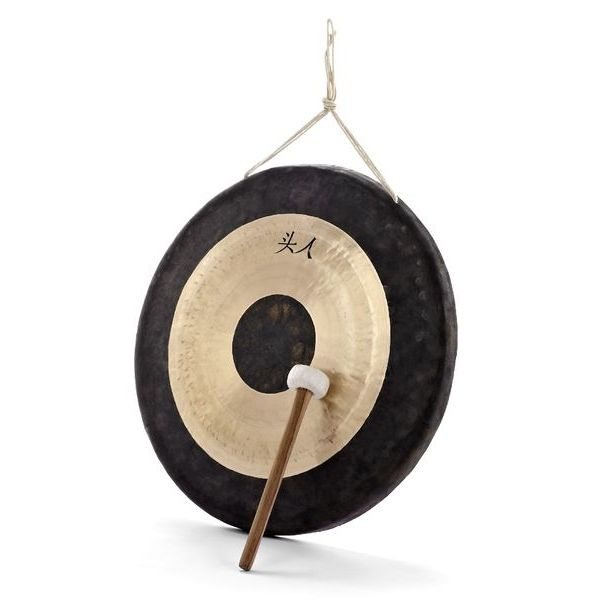
\includegraphics[width=\linewidth]{Chapters/tam-tam.png}
        \caption{Tam-tam}
        \label{fig:image1}
    \end{minipage}
    \hfill
    \begin{minipage}{0.45\linewidth}
        \centering
        
\includegraphics[width=\linewidth]{logos/tamtam.png}
        \caption{logo Tamtam international}
        \label{fig:image2}
    \end{minipage}
\end{figure}

\subsection{Activité de tamtam International}
L'entreprise Tamtam se distingue des autres entreprises sur le marché par sa philosophie ; elle ne
se spécialise pas dans le développement de solutions informatiques pour d'autres clients à la
demande, mais elle se focalise sur le développement d'un écosystème pour la gestion de
communautés et vise à devenir le leader sur le marché.
\subsection{Produits de Tamtam International}
Les produits offerts par Tamtam sont variés et visent à créer un écosystème complet pour la
gestion efficace des communautés. Chaque produit est conçu pour répondre à des besoins
spécifiques, allant de la communication interne à l'engagement des membres. En intégrant ces
solutions, Tamtam permet aux utilisateurs de centraliser les interactions, de faciliter la
coordination et d'améliorer la collaboration au sein de leurs communautés. L'objectif principal est de fournir des outils qui soutiennent la croissance et le dynamisme des groupes, tout en
simplifiant la gestion quotidienne et en renforçant les liens entre les membres.
\begin{figure}[htbp!]

    \hspace{4cm} % Décalage horizontal
    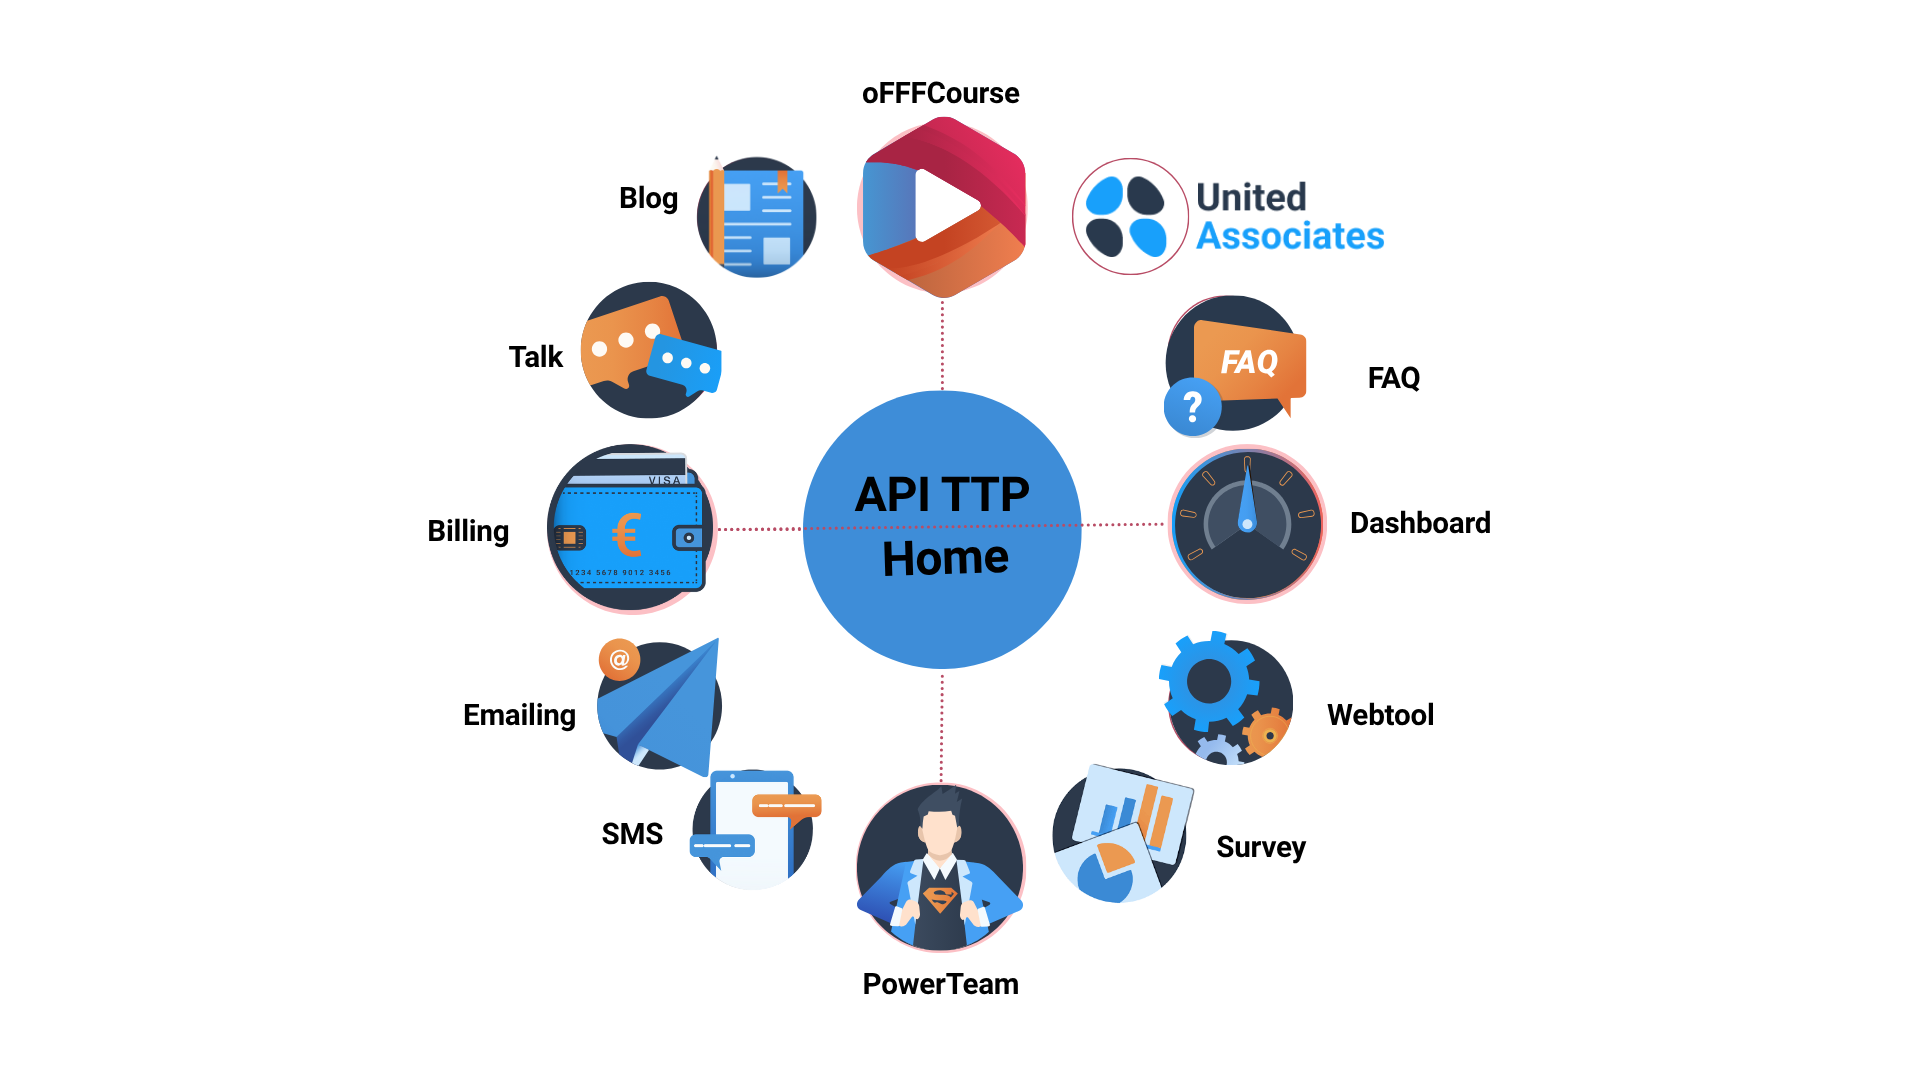
\includegraphics[width=1.55\linewidth, right]{Chapters/produitsTamtam.png}
    \caption{produit tamtam internationel}
    \label{fig:enter-label}
\end{figure}

\textbf{Home} : Cette application centrale représente l’interface d’authentification pour toutes les
applications de Tamtam. Elle gère les différents utilisateurs des organisations en leur offrant la
possibilité d’activer etde configurer les différentes applications disponibles pour chaque profil
utilisateur.

\textbf{Emailling} : Une application permettant à un client d’envoyer des compagnes (des emails) à des
contacts (des utilisateurs stockés dans la base de données dans ttp-users qui ont un email).

\textbf{Blog} : Une application offrant un espace personnel à un utilisateur pour rédiger ses articles,
consulter d’autres articles, ainsi que choisir les organisations qui peuvent le consulter.

\textbf{oFFcourse} : Une application web ayant une partie mobile gérant les événements (conférences,
formations) pour des fiduciaires situés à Belgique. Le visiteur peut consulter le planning, les
orateurs, les places disponibles et s’inscrire à une formation ou réserver une place à une
conférence en choisissant une formule précise parmi celles proposées, ou bien en proposant un
événement.

\textbf{Talk} : est une application interne pour le moment, elle prend automatiquement les clients et
collègues de la personne connectée à Home. Les utilisateurs peuvent chatter, passer des appels
audio et vidéo et envoyer des documents.

\textbf{Billing} : est un moteur de routage permettant le transfert et l’acheminement des
documents électroniques vers la bonne destination, tout en prenant en considération le métier et
les besoins des experts comptables. Un document électronique peut être une facture sous format

\textbf{Efff} ou\textbf{PDF}, un bulletin de paie ou un document bancaire de type Coda.
Paiement : Cette application permet aux clients Tamtam d’effectuer le payement des
évènements ainsi que des produits qu’ils désirent obtenir, elle regroupe deux types de payement
en ligne et prend en charge les virements.

\textbf{Survey} : une application web qui permet de fournir une plateforme pour générer des
questionnaires afin d'offrir à tous les fiduciaires belges les moyens nécessaires pour consulter la
satisfaction de ces clients. De plus gérer les données et les réponses par des Dashboard avec
graphiques et statistiques, qui montreront de manière synthétique les résultats de chaque
questionnaire.

\textbf{SMS} : une application permettant à chaque client (organisation, fiduciaire) d'envoyer des sms à
ses clients qui sont stockés dans la base de données Tamtam qui ont un numéro de téléphone.
Afin de leur permettre de connaître par exemple les dates et thèmes des évènements, les
nouveautés, etc. Cette application utilise une api externe qui s'appelle MessageBird.

\textbf{workflow} : une application permet de piloter les résultats par une réconciliation des tâches
effectuées et de déterminer qui et où se produit la valeur ajoutée et de maximiser la charge à
facturer au client en tenant compte des éventuels gains de productivité.

\textbf{E-zine} : une extension de Blog, elle est accessible juste pour des utilisateurs qui ont un compte,
en lui offrant la possibilité de partager des articles dans les réseaux sociaux et intégrer des
articles externes...

\textbf{Efff-viewe}r : une application gérant la validation des factures au format efff. Ce format est né
le 7 juillet 2012, basé sur l’UBL 2.0 il limite considérablement les champs (réduits à 200
potentiels) et consacre une même interprétation de toutes les maisons de softwares. Un langage
commun voit le jour et permet dorénavant à la majorité des logiciels comptables et de gestion
(80 % du marché) d’émettre et de recevoir sous un même format une facture électronique.
PowerTeam: est une application conçue pour la gestion complète des relations entre les clients
et leurs collaborateurs. Elle offre des fonctionnalités pour la gestion des collaborateurs, leurs
budgets ainsi qu'un outil de suivi des prestations afin d'optimiser leur rendement.

\subsection{Clients de Tamtam International}

Les principaux clients de Tamtam International sont les organisations des fiduciaires et expert-comptable en Belgique, les principaux clients sont :


\begin{itemize}
    \item \textbf{\textbf{IEC }: }Institut des Experts-comptables et des Conseils fiscaux – Belgique.
    \item \textbf{\textbf{UP (UnifiedPost) }: }société belge leader dans le secteur des fintechs.
    \item \textbf{\textbf{Deg \& Partners }:} C'est un bureau comptable en pleine croissance, spécialisé dans les professions libérales, les artistes et les ASBL (association sans but lucratif), et expert dans le passage.
    \item \textbf{FFF (Forum For the Futur) }: le congrés Forum for the Futur est le rendez-vous annuel des professions économiques.
    \item \textbf{ITAA (Institute for Tax Advisors \& Accountants) }: Institut des comptables et des conseillers fiscaux, Belgique.
\end{itemize}

\begin{figure}[htbp]
    \centering
    
\includegraphics[width=1\linewidth]{Chapters/image.png}
    \caption{Clients de Tamtam International}
    \label{fig:enter-label}
\end{figure}
\section{Présentation du projet de stage}
Durant mon passage chez Tamtam International, j’ai eu la chance de contribuer à un projet clé reflétant la volonté de l’entreprise de s’adapter aux attentes diversifiées de sa clientèle fiduciaire en Belgique.

\subsection{Contexte général du projet}

Tamtam Pro se positionne comme une plateforme belge innovante, dédiée à l'accompagnement des professionnels fiduciaires à travers le pays. La particularité de cette structure réside dans son approche modulaire, où chaque projet répond à des besoins sectoriels distincts, nécessitant une adaptation permanente de la part des équipes techniques.

Face à l'expansion continue de l'entreprise, plusieurs fonctionnalités stratégiques ont été progressivement implémentées. Parmi ces développements clés, on retrouve notamment des outils avancés de gestion budgétaire et d'optimisation de la capacité productive, spécialement conçus pour les cabinets fiduciaires.

Cette initiative s'inscrit dans la philosophie d'innovation permanente qui caractérise Tamtam International, avec pour vocation d'anticiper les évolutions du marché belge des services financiers. Les solutions développées s'adressent principalement aux entreprises partenaires du réseau Tamtam, particulièrement aux fiduciaires qui exercent une activité à forte intensité cognitive et opérationnelle.

La création de ces outils répondait à un double impératif :
 \begin{enumerate}
     \item Simplifier les processus métiers exigeants.
     \item Optimiser le ratio effort/rendement professionnel.
 \end{enumerate}

Structurellement, Tamtam opère actuellement à travers deux pôles complémentaires :
\begin{itemize}
    \item oFFcourse.be (équipe d'accueil de mon PFE)
    \item UnitedAssociate.be
\end{itemize}

\subsubsection{Objectifs du projet de fin d'études}
Mon intervention s'articule autour de deux axes principaux :
 \begin{enumerate}
     \item L'optimisation des fonctionnalités existantes pour répondre aux nouvelles attentes utilisateurs.
     \item Le développement d'un système LMS dédié au management des compétences, permettant :\begin{itemize}
     \item La définition d'objectifs formatifs trimestriels (en heures-crédits).
   \item Un mécanisme de recommandation intelligente de parcours pédagogiques.
  \item Le suivi granularisé des progressions individuelles.
     \end{itemize}
 \end{enumerate}

\subsection{Problématique}
Aujourd’hui, le marché belge de la formation fiduciaire devient de plus en plus concurrentiel, avec des exigences croissantes en matière de suivi et de personnalisation des apprentissages. Face à cette évolution, Tamtam Pro cherche à renforcer son écosystème en y intégrant une nouvelle interface LMS complète, capable de répondre aux besoins spécifiques des fiduciaires.

La question centrale se pose alors : comment Tamtam Pro peut-il réussir cette transition vers un système plus performant, tout en gardant son avantage concurrentiel ?

D’une part, il s’agit d’automatiser le suivi des obligations de formation continues, un enjeu clé pour les fiduciaires soumis à des réglementations strictes. D’autre part, le système doit personnaliser les parcours d’apprentissage en fonction des profils métiers, permettant ainsi à chaque collaborateur de progresser efficacement.

Enfin, cette solution doit se différencier des plateformes existantes, en offrant une flexibilité accrue et des outils de reporting avancés, adaptés aux réalités opérationnelles des cabinets fiduciaires.

En résumé, le défi consiste à concevoir un LMS qui soit à la fois structuré, personnalisable et intégré harmonieusement dans l’écosystème Tamtam, tout en répondant aux attentes précises des professionnels du secteur.

\subsection{Étude des solutions existantes sur le Marché}
\label{sec:solutions-existantes}

Dans le domaine des \textbf{Learning Management Systems (LMS)} dédiés aux fiduciaires et aux métiers réglementés, plusieurs solutions se démarquent. Cette analyse comparative permet d'identifier les \textbf{forces et faiblesses} des plateformes concurrentes, tout en mettant en lumière les \textbf{opportunités d'innovation} pour Tamtam Pro.

\subsubsection{Plateformes généralistes (LMS polyvalents)}
\begin{itemize}
    \item \textbf{Moodle, LearnDash, TalentLMS}
    \begin{itemize}
        \item[\checkmark] \textbf{Avantages} : flexibilité, personnalisation des parcours, outils de suivi basiques.
        \item[\texttimes] \textbf{Limites} : non adaptés spécifiquement aux besoins des fiduciaires.
    \end{itemize}
\end{itemize}

\subsubsection{Solutions spécialisées pour les fiduciaires}
\begin{itemize}
    \item \textbf{FiscalTalent (payroll \& legal training)}
    \begin{itemize}
        \item[\checkmark] \textbf{Points forts} : contenus préétablis pour les formations fiscales.
        \item[\texttimes] \textbf{Défis} : rigidité dans la gestion des objectifs
    \end{itemize}
    
    \item \textbf{Acerta Academy}
    \begin{itemize}
        \item[\checkmark] \textbf{Atouts} : intégration avec les outils RH
        \item[\texttimes] \textbf{Faiblesses} : interface peu intuitive.
    \end{itemize}
\end{itemize}

\subsubsection{Analyse des lacunes du marché}
Les solutions actuelles présentent \textbf{trois principales limites} :
\begin{enumerate}
    \item Manque d'adaptation aux cycles trimestriels
    \item Absence de mécanismes intelligents de recommandation
    \item Peu de flexibilité dans le suivi des formations hybrides.
\end{enumerate}

\subsubsection{Positionnement de Tamtam Pro}
Pour se différencier, le futur LMS \textbf{« Didier »} devra :
\begin{itemize}
    \item[\textbullet] Combler les lacunes des solutions existantes.
    \item[\textbullet] Offrir une expérience unifiée dans l'écosystème Tamtam.
    \item[\textbullet] Automatiser le suivi avec personnalisation fine.

\end{itemize}

\begin{quote}
\textit{Cette étude confirme l'opportunité stratégique pour Tamtam Pro de développer une solution à la fois spécialisée, intuitive et intégrée, répondant mieux aux attentes des fiduciaires que les alternatives actuelles.}
\end{quote}

\section{Conduite de projet}
La gestion et la planification de projet constituent le pilier central pour mener à bien toute initiative. Une démarche méthodique s'impose pour structurer l'ensemble des activités, depuis l'identification précise des tâches jusqu'à leur séquencement optimal. Ce processus exige notamment d'évaluer avec justesse la durée nécessaire pour chaque action et d'établir une chronologie rigoureuse des phases. Cette approche disciplinée permet non seulement de cadrer efficacement le déroulement des opérations, mais aussi de maîtriser les délais et d'anticiper les éventuels aléas. Dans le cadre de notre projet LMS, cette méthodologie prend tout son sens pour garantir une implémentation fluide et conforme aux attentes.
\subsection{Méthodologie de travail}
Le choix d'une méthodologie adaptée constitue un facteur clé de succès pour tout projet informatique, permettant à l'ensemble des acteurs de collaborer efficacement selon des règles bien définies. Cette sélection stratégique doit répondre précisément aux spécifications du projet tout en garantissant un produit final conforme aux attentes clients. Chez Tamtam International, nous avons opté pour Scrum comme méthodologie de référence, pour plusieurs raisons déterminantes : son efficacité éprouvée dans divers contextes projet, sa capacité à se rapprocher au plus près des besoins clients, sa simplicité de mise en œuvre, et la transparence qu'elle offre sur l'avancement des travaux. Cette approche agile permet non seulement d'optimiser la qualité des livrables, mais aussi de maintenir une visibilité constante sur l'état du projet.
\subsection{Répartition des rôles}

Le cadre Scrum distingue trois types de participants :

\begin{table}[h]
  \centering
  \caption{Cycle de vie Scrum}
  \label{tab:cycle-vie-scrum}
  \begin{tabular}{p{4cm} p{10cm}}
    \toprule
    \textbf{Acteur} & \textbf{Description} \\\\
    \midrule
    Product Owner &
      Il est incarné par Monsieur Emmanuel DEGRÈVE.
      Il apporte l’expertise fonctionnelle et opère les arbitrages indispensables à la priorisation des développements. \\
      \\
    \addlinespace
    Scrum Master &
      Il est incarné par Monsieur Youssef IDBRAIM, membre de l’équipe,
      et sa mission principale est d’optimiser la capacité de production
      de l’équipe en l’accompagnant dans une amélioration continue. \\
      \\
    \addlinespace
    Équipe de développement &
      Elle prend en charge la réalisation du produit (planification,
      conception, codage, tests, documentation) sans spécialisation des
      rôles. La particularité d’une équipe Scrum est d’être « auto-organisée »,
      et donc dépourvue de toute hiérarchie. \\
    \bottomrule
  \end{tabular}
\end{table}

Étant donné que Scrum suit un processus itératif, les unités de temps centrales sont le \textbf{Sprint} et la \textbf{Release}.\\

Dans le cadre du projet \textit{Tamtam}, une nouvelle approche est adoptée cette année avec une Release de 6 semaines, au lieu de 4. Cette Release comprend 4 Sprints :\\
- Deux Sprints principaux de 2 semaines chacun \\
- Deux Sprints appelés \textit{Sprint-Release} d’une semaine chacun, dédiés à la mise en production, à la finalisation de la documentation, et à la prise en compte des retours des parties prenantes.\\

Le contenu de cette Release est fixé lors d’une réunion de planification initiale, garantissant ainsi son périmètre.

\subsection{Workflow
}
Nous explorerons les principes fondamentaux de Scrum, une méthodologie Agile populaire pour
la gestion de projets. Cela inclut une compréhension approfondie des rôles, des événements et
des artefacts de Scrum, ainsi qu'une analyse de son workflow typique, qui guide les équipes à
travers les phases de planification, de développement, de revue et de rétrospective.
\begin{figure}[htbp]
    \centering
    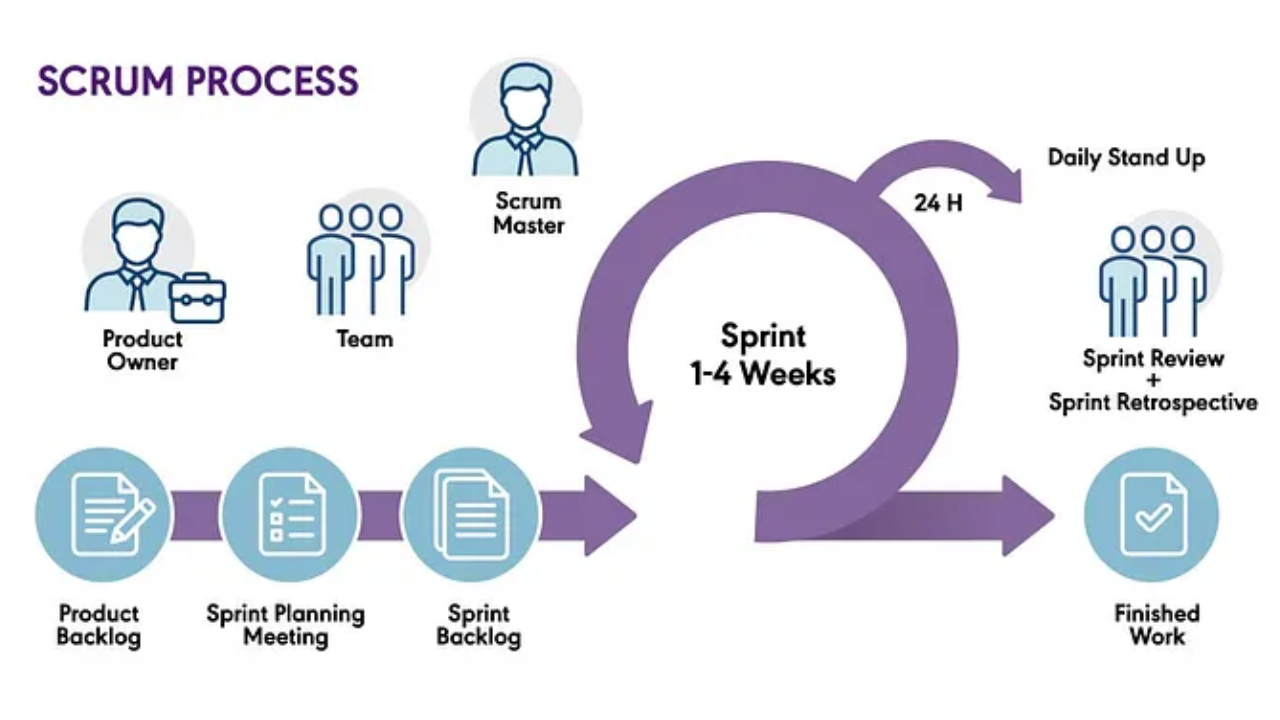
\includegraphics[width=1\linewidth]{Titre de la présentation[1].pdf.png}
    \caption{Cycle de vie SCRUM}
    \label{fig:enter-label}
\end{figure}
\subsubsection{Sprint planning:}
Sprint planning est une étape clé dans la méthodologie agile, particulièrement dans le cadre de
Scrum. Elle vise à définir le travail à accomplir lors du prochain sprint.
Figure 11 Sprint Planning meeting

- L'équipe se réunit pour étudier les exigences fonctionnelles.
- Les fonctionnalités sont divisées en tâches.
- Chaque tâche est attribuée un point par la méthode du planning poker qui représente sa
difficulté.
- Les tâches sont distribuées sur l'ensemble de l'équipe en fonction de l'expertise et des
compétences de chacun.
\subsubsection{Sprint review:}
La Sprint review, dernière étape de chaque sprint Scrum, offre l'opportunité d'examiner
l'incrément de produit. Elle permet à l'équipe de présenter ses réalisations aux parties prenantes,
de recueillir leurs retours et d'ajuster le backlog produit en conséquence. Cette réunion favorise
la transparence et la collaboration, garantissant que le produit évolue de manière alignée sur les
besoins du client tout au long du processus de développement.\\
- L'équipe s'assemble pour présenter une démonstration au PO (Product Owner).\\
- Le PO valide l'état d'avancement et propose des changements.\\
- Le PO spécifie aussi et explique le BR (Business Requirement) à développer pour le
prochain sprint.\\
Durant cette période de stage, nous avions l’habitude d’effectuer deux autres types de réunions :
\subsubsection{Stand up meeting (Daily scrum meeting):}
Chaque jour, nous faisions une petite réunion avec le Scrum master, pour savoir ce qui a été
complété, ce qui est en cours ou planifié, les problèmes et obstacles rencontrés.

\subsubsection{La réunion de rétrospective (Sprint retrospective):}
La rétrospective eut lieu juste après la sprint review, pour discuter le feed-back sur ce qui a été
réalisé, proposer des améliorations du produit, planifier le prochain sprint et assigner les
nouvelles tâches.

\subsection{Gestion des tâches et suivis}
Au sein de notre équipe, Notion joue un rôle central dans la gestion, la collaboration et le suivi
de nos projets. Cet outil polyvalent nous permet de structurer nos tâches, de collaborer de
manière efficace et de maintenir une visibilité claire sur l'avancement de nos projets. Grâce à ses
fonctionnalités flexibles, nous pouvons personnaliser notre espace de travail pour répondre aux
besoins spécifiques de chaque projet, ce qui contribue à une gestion efficace des ressources et à
une coordination harmonieuse des efforts d'équipe.
\begin{figure}[hb!]
    \centering
    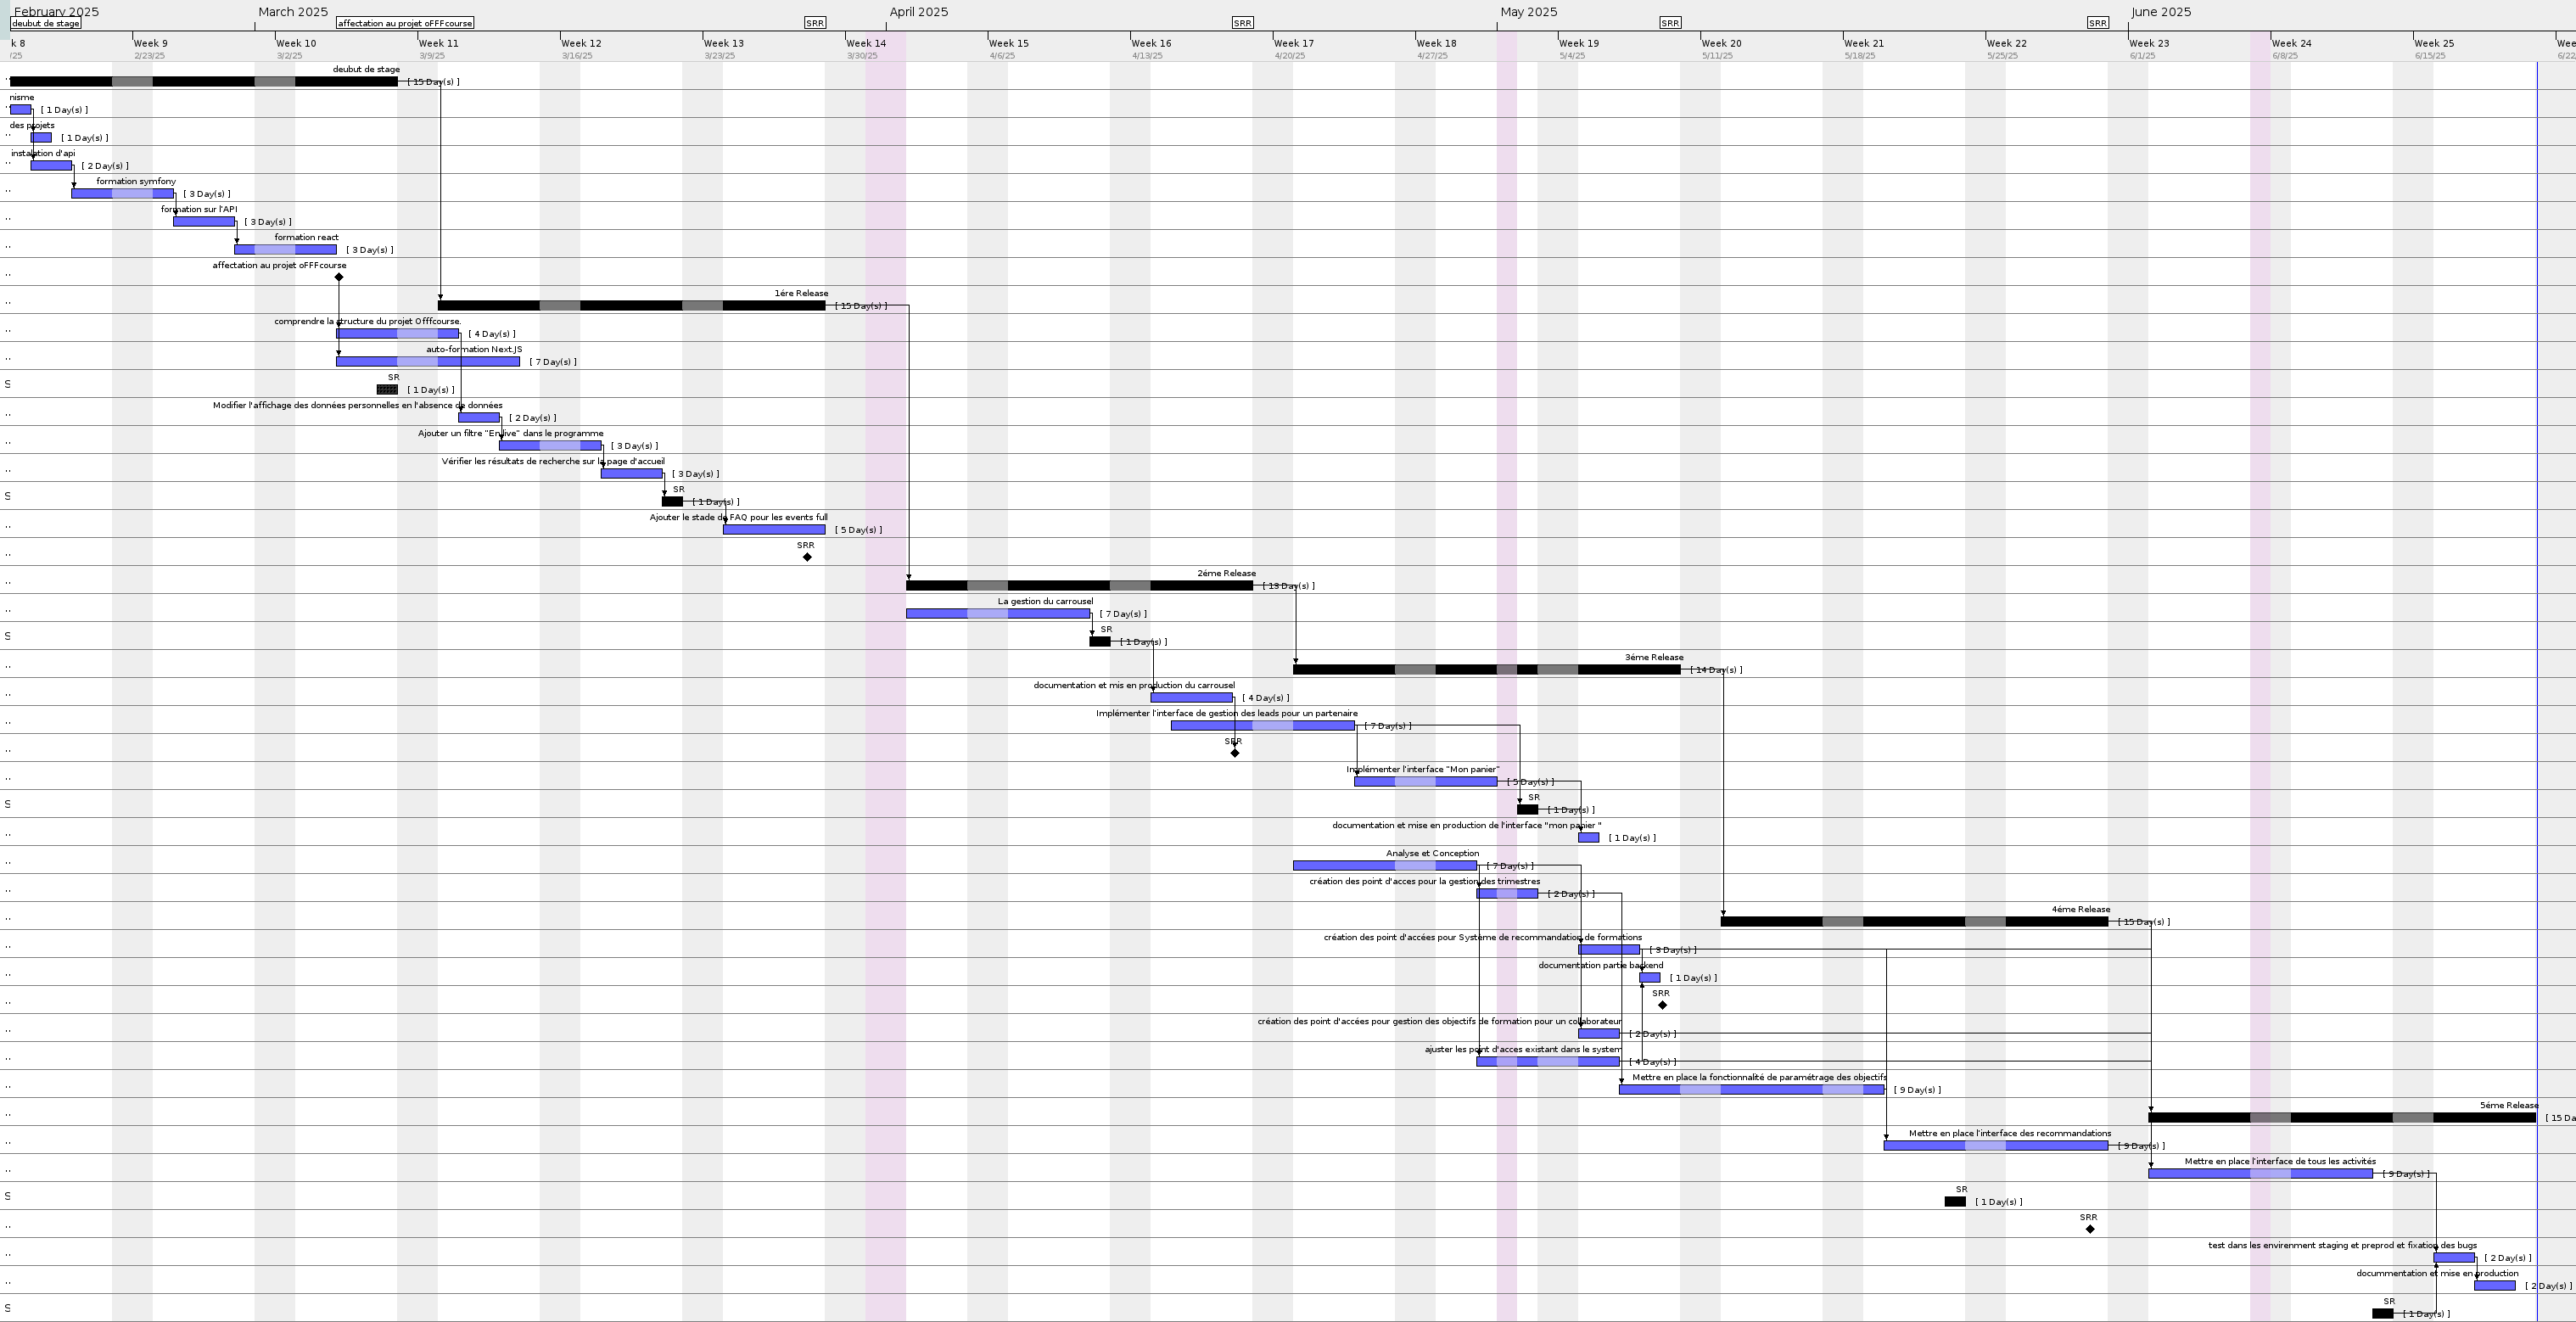
\includegraphics[width=1\linewidth]{pfeProject.gan_page0.png}
    \caption{diagramme de gant }
    \label{fig:enter-label}
\end{figure}
\subsection{Description du diagramme de Gantt}

Ce diagramme de Gantt présente la planification détaillée du projet sur une période de 5 mois (février à juin 2025), intégrant à la fois les tâches liées au développement du système LMS et d'autres activités de l'équipe Tamtam. La structure reflète l'approche Scrum avec des sprints de 2 semaines.

\textbf{Tâches identifiées dans le diagramme :}

\textbf{Sprint 1-2 (Février - début Mars) - Tâches autour oFFFcourse :}
\begin{itemize}
    \item Configuration de l'environnement de développement
    \item Maintenance et amélioration des applications existantes (oFFcourse, Blog, etc.)
    \item Résolution de bugs critiques sur les modules Tamtam
    \item Mise à jour des dépendances techniques
\end{itemize}

\textbf{Sprint 3-4 (Mi-Mars - début Avril) - Début des tâches LMS :}
\begin{itemize}
    \item Analyse des besoins fonctionnels du LMS
    \item Étude des solutions existantes sur le marché
    \item Conception de l'architecture système
    \item Définition des user stories et du backlog produit
    \item Création des maquettes et prototypes UI/UX
\end{itemize}

\textbf{Sprint 5-6 (Avril) - Développement core LMS :}
\begin{itemize}
    \item Implémentation du système d'authentification
    \item Développement du module de gestion des utilisateurs
    \item Création de la base de données des formations
    \item Développement de l'interface d'administration
\end{itemize}

\textbf{Sprint 7-8 (Mai) - Fonctionnalités avancées LMS :}
\begin{itemize}
    \item Implémentation du système de recommandations
    \item Développement du module de suivi des objectifs trimestriels
    \item Création des tableaux de bord et reporting
    \item Intégration avec l'écosystème Tamtam existant
\end{itemize}

\textbf{Sprint 9-10 (Juin) - Finalisation et déploiement :}
\begin{itemize}
    \item Tests d'intégration et de performance
    \item Documentation technique et utilisateur
    \item Formation des utilisateurs finaux
    \item Déploiement en production et mise en ligne
\end{itemize}

Cette planification montre clairement que le développement du LMS représente environ 70\% du temps total du projet, les 30\% restants étant consacrés aux formations et aux activités de maintenance et d'amélioration de l'écosystème Tamtam existant.

\section{Conclusion}

Ce premier chapitre a permis d'établir les fondements solides de notre projet de fin d'études au sein de Tamtam International. L'exploration approfondie de l'organisme d'accueil révèle une entreprise innovante, positionnée comme acteur de référence dans l'écosystème numérique des fiduciaires belges.

La présentation de Tamtam International met en évidence sa philosophie unique : plutôt que de développer des solutions sur mesure pour des tiers, l'entreprise se concentre sur la création d'un écosystème intégré de produits, visant l'excellence dans la gestion de communautés professionnelles. Cette approche stratégique, incarnée par la vision de son fondateur Emmanuel Degrève, positionne Tamtam comme un partenaire technologique de confiance pour les professionnels du secteur fiduciaire.

L'analyse du contexte projet révèle une opportunité stratégique majeure : le développement d'un système LMS spécialisé pour répondre aux besoins croissants de formation continue des fiduciaires. L'étude comparative des solutions existantes confirme l'existence d'un gap technologique que le projet « Didier » ambitionne de combler, en proposant une approche à la fois personnalisée, intuitive et parfaitement intégrée à l'écosystème Tamtam.

La méthodologie Scrum adoptée, avec sa structure de sprints et de releases adaptée aux spécificités du projet, garantit une approche itérative et collaborative. La planification détaillée, matérialisée par le diagramme de Gantt, démontre la faisabilité technique du projet dans les délais impartis, tout en préservant la qualité des livrables.

Fort de ces bases solides, nous sommes désormais en mesure d'aborder les phases techniques du projet avec confiance. Le chapitre suivant se concentrera sur l'analyse approfondie des besoins fonctionnels et non-fonctionnels, préalable indispensable à la conception d'une solution technologique performante et adaptée aux attentes des utilisateurs finaux.
\chapter{Analyse et Conception}

L'analyse et la conception constituent les phases cruciales dans le développement de tout système d'information. Cette étape permet de transformer les besoins exprimés par les utilisateurs en spécifications techniques détaillées, servant de base solide pour l'implémentation du système.

Dans le contexte de notre projet de développement d'un système LMS (Learning Management System) pour OffCourse et United Associate, ce chapitre présente une approche méthodique et rigoureuse pour analyser les besoins fonctionnels et non fonctionnels du système. Nous utiliserons le langage de modélisation UML (Unified Modeling Language) pour représenter visuellement l'architecture et le comportement du système.

L'objectif principal de cette phase d'analyse est de :
\begin{itemize}
    \item Identifier et formaliser les besoins des différents acteurs du système
    \item Définir les fonctionnalités essentielles du système LMS
    \item Modéliser les interactions entre les utilisateurs et le système
    \item Établir une architecture logique claire et évolutive
    \item Préparer les bases techniques pour la phase d'implémentation
\end{itemize}

Cette approche méthodologique nous permettra de garantir que le système développé répond parfaitement aux attentes des utilisateurs tout en respectant les contraintes techniques et organisationnelles.

\section{Langage de modélisation UML2}

\subsection{Présentation d'UML}

UML (Unified Modeling Language) est un langage de modélisation graphique standardisé utilisé pour spécifier, visualiser, construire et documenter les systèmes logiciels. Créé dans les années 1990 par Grady Booch, James Rumbaugh et Ivar Jacobson, UML est devenu le standard de facto pour la modélisation orientée objet.

\begin{figure}[htbp]
\centering

\includegraphics[width=0.3\linewidth]{uml-logo.png}
\caption{Logo UML - Unified Modeling Language}
\end{figure}

\subsection{Avantages d'UML pour notre projet}

L'adoption d'UML pour la conception de notre système LMS présente plusieurs avantages :

\textbf{\textbullet\ Standardisation :} UML est un langage normalisé reconnu internationalement, facilitant la communication entre les différents acteurs du projet.

\textbf{\textbullet\ Expressivité :} Les diagrammes UML permettent de représenter différents aspects du système (structure, comportement, interactions) de manière claire et précise.

\textbf{\textbullet\ Indépendance technologique :} UML est indépendant des langages de programmation et des plateformes, permettant une conception abstraite du système.

\textbf{\textbullet\ Support de communication :} La notation graphique d'UML facilite les discussions entre les équipes techniques et les parties prenantes non techniques.

\subsection{Diagrammes UML utilisés}

Pour notre système LMS, nous utiliserons principalement :
\begin{itemize}
    \item \textbf{Diagrammes de cas d'utilisation} : pour identifier les fonctionnalités du système
    \item \textbf{Diagrammes de séquence} : pour modéliser les interactions temporelles
    \item \textbf{Diagrammes de classes} : pour représenter la structure statique du système
    \item \textbf{Diagramme Bête à Cornes} : pour analyser la finalité du système
\end{itemize}

\section{Capture des besoins}

\subsection{Méthodologie de capture des besoins}

La capture des besoins est une étape fondamentale qui détermine la réussite du projet. Une mauvaise compréhension des besoins peut conduire au développement d'un système inadapté, entraînant des coûts supplémentaires et des retards significatifs.

Notre approche de capture des besoins s'appuie sur :
\begin{itemize}
    \item Des entretiens avec les parties prenantes (administrateurs, collaborateurs, utilisateurs)
    \item L'analyse des processus métier existants
    \item L'étude des systèmes similaires
    \item La définition de scénarios d'usage concrets
\end{itemize}

\subsection{Besoins fonctionnels}

Les besoins fonctionnels décrivent les services que le système doit fournir, ses réactions aux entrées particulières et son comportement dans des situations spécifiques.

\subsubsection{Gestion des formations (Utilisateur Simple)}

L'utilisateur simple dispose des fonctionnalités suivantes pour gérer son parcours de formation :

\begin{itemize}
    \item \textbf{Consultation des formations} : Accès au catalogue complet des formations disponibles avec descriptions détaillées
    \item \textbf{Suivi des progrès} : Visualisation de l'avancement dans chaque formation entreprise
    \item \textbf{Gestion du panier} : Ajout/suppression de formations dans un panier d'achat
    \item \textbf{Consultation des factures} : Accès à l'historique des achats et des facturations
    \item \textbf{Définition d'objectifs personnels} : Établissement d'objectifs d'heures de formation par trimestre
    \item \textbf{Suivi des objectifs} : Monitoring de la progression vers les objectifs fixés
    \item \textbf{Statistiques d'intérêts} : Consultation d'un nuage de mots-clés représentant les domaines d'intérêt
\end{itemize}

\subsubsection{Gestion des objectifs organisationnels (Collaborateur)}

Le collaborateur, membre d'une organisation, bénéficie de fonctionnalités spécifiques :

\begin{itemize}
    \item \textbf{Consultation des objectifs assignés} : Visualisation des objectifs définis par l'administrateur
    \item \textbf{Formations recommandées} : Accès à la liste des formations suggérées par l'organisation
    \item \textbf{Suivi organisationnel} : Monitoring des progrès dans le cadre des objectifs de l'organisation
    \item \textbf{Distinction des formations} : Classification claire entre formations spontanées et recommandées
\end{itemize}

\subsubsection{Administration LMS (Administrateur Premium)}

L'administrateur premium dispose de privilèges étendus pour gérer l'organisation :

\begin{itemize}
    \item \textbf{Gestion des trimestres} : Configuration des périodes de formation organisationnelles
    \item \textbf{Définition d'objectifs} : Assignation d'objectifs d'heures spécifiques aux collaborateurs
    \item \textbf{Recommandations de formations} : Création de recommandations (obligatoires, suggestions, spontanées)
    \item \textbf{Suivi global des progrès} : Monitoring de l'avancement de tous les collaborateurs
    \item \textbf{Validation des formations} : Possibilité de marquer une formation comme terminée
    \item \textbf{Consultation détaillée} : Accès aux profils et statistiques de chaque collaborateur
\end{itemize}

\subsection{Besoins non fonctionnels}

Les besoins non fonctionnels définissent les critères de qualité que le système doit respecter pour assurer son bon fonctionnement en conditions réelles.

\subsubsection{Ergonomie et accessibilité}

Le système doit proposer une interface intuitive adaptée aux utilisateurs de tous niveaux techniques. L'ergonomie est cruciale pour l'adoption du système par les collaborateurs.

\subsubsection{Performance et scalabilité}

Le système doit maintenir des temps de réponse acceptables même avec un nombre croissant d'utilisateurs et de données. L'architecture doit supporter la montée en charge.

\subsubsection{Sécurité et confidentialité}

La protection des données personnelles et professionnelles est primordiale. Le système doit garantir l'intégrité et la confidentialité des informations des utilisateurs et des organisations.

\subsubsection{Fiabilité et robustesse}

Le système doit fonctionner de manière stable, gérer les erreurs gracieusement et assurer la continuité de service même en cas de surcharge.

\section{Identification des acteurs}

L'identification des acteurs est essentielle pour définir les frontières du système et comprendre les différents types d'interactions possibles.

\begin{table}[htbp]
\centering
\begin{tabular}{|p{3cm}|p{10cm}|}
\hline
\textbf{Acteur} & \textbf{Description et rôles} \\
\hline
\textbf{Utilisateur Simple} & 
Collaborateur individuel qui utilise le système pour son développement personnel. Il accède aux formations, gère son panier d'achat, consulte ses factures, définit ses objectifs personnels et suit ses progrès de manière autonome. \\
\hline
\textbf{Collaborateur} & 
Utilisateur membre d'une organisation qui, en plus des fonctionnalités de base, peut accéder aux formations recommandées par son administrateur, consulter les objectifs organisationnels qui lui sont assignés et suivre ses progrès dans le cadre de sa structure. \\
\hline
\textbf{Administrateur Premium} & 
Responsable d'une organisation avec des privilèges étendus. Il peut gérer les trimestres organisationnels, définir des objectifs pour ses collaborateurs, recommander des formations (obligatoires ou suggestions), suivre les progrès de son équipe et valider les formations accomplies. \\
\hline
\end{tabular}
\caption{Identification et description des acteurs du système LMS}
\end{table}

\section{Diagrammes UML}
Dans cette section, nous plongerons dans l'univers des diagrammes UML. Nous examinerons
comment chaque type de diagramme peut être utilisé pour modéliser différents aspects d'un
système logiciel, de la structure des classes à la séquence des interactions entre les objets.
\subsection{Diagramme Bête à Cornes}

Le diagramme Bête à Cornes nous permet d'analyser la finalité du système en répondant aux questions fondamentales : à qui rend-il service, sur quoi agit-il, et dans quel but.

\hfill
\begin{figure}[htb]
\centering
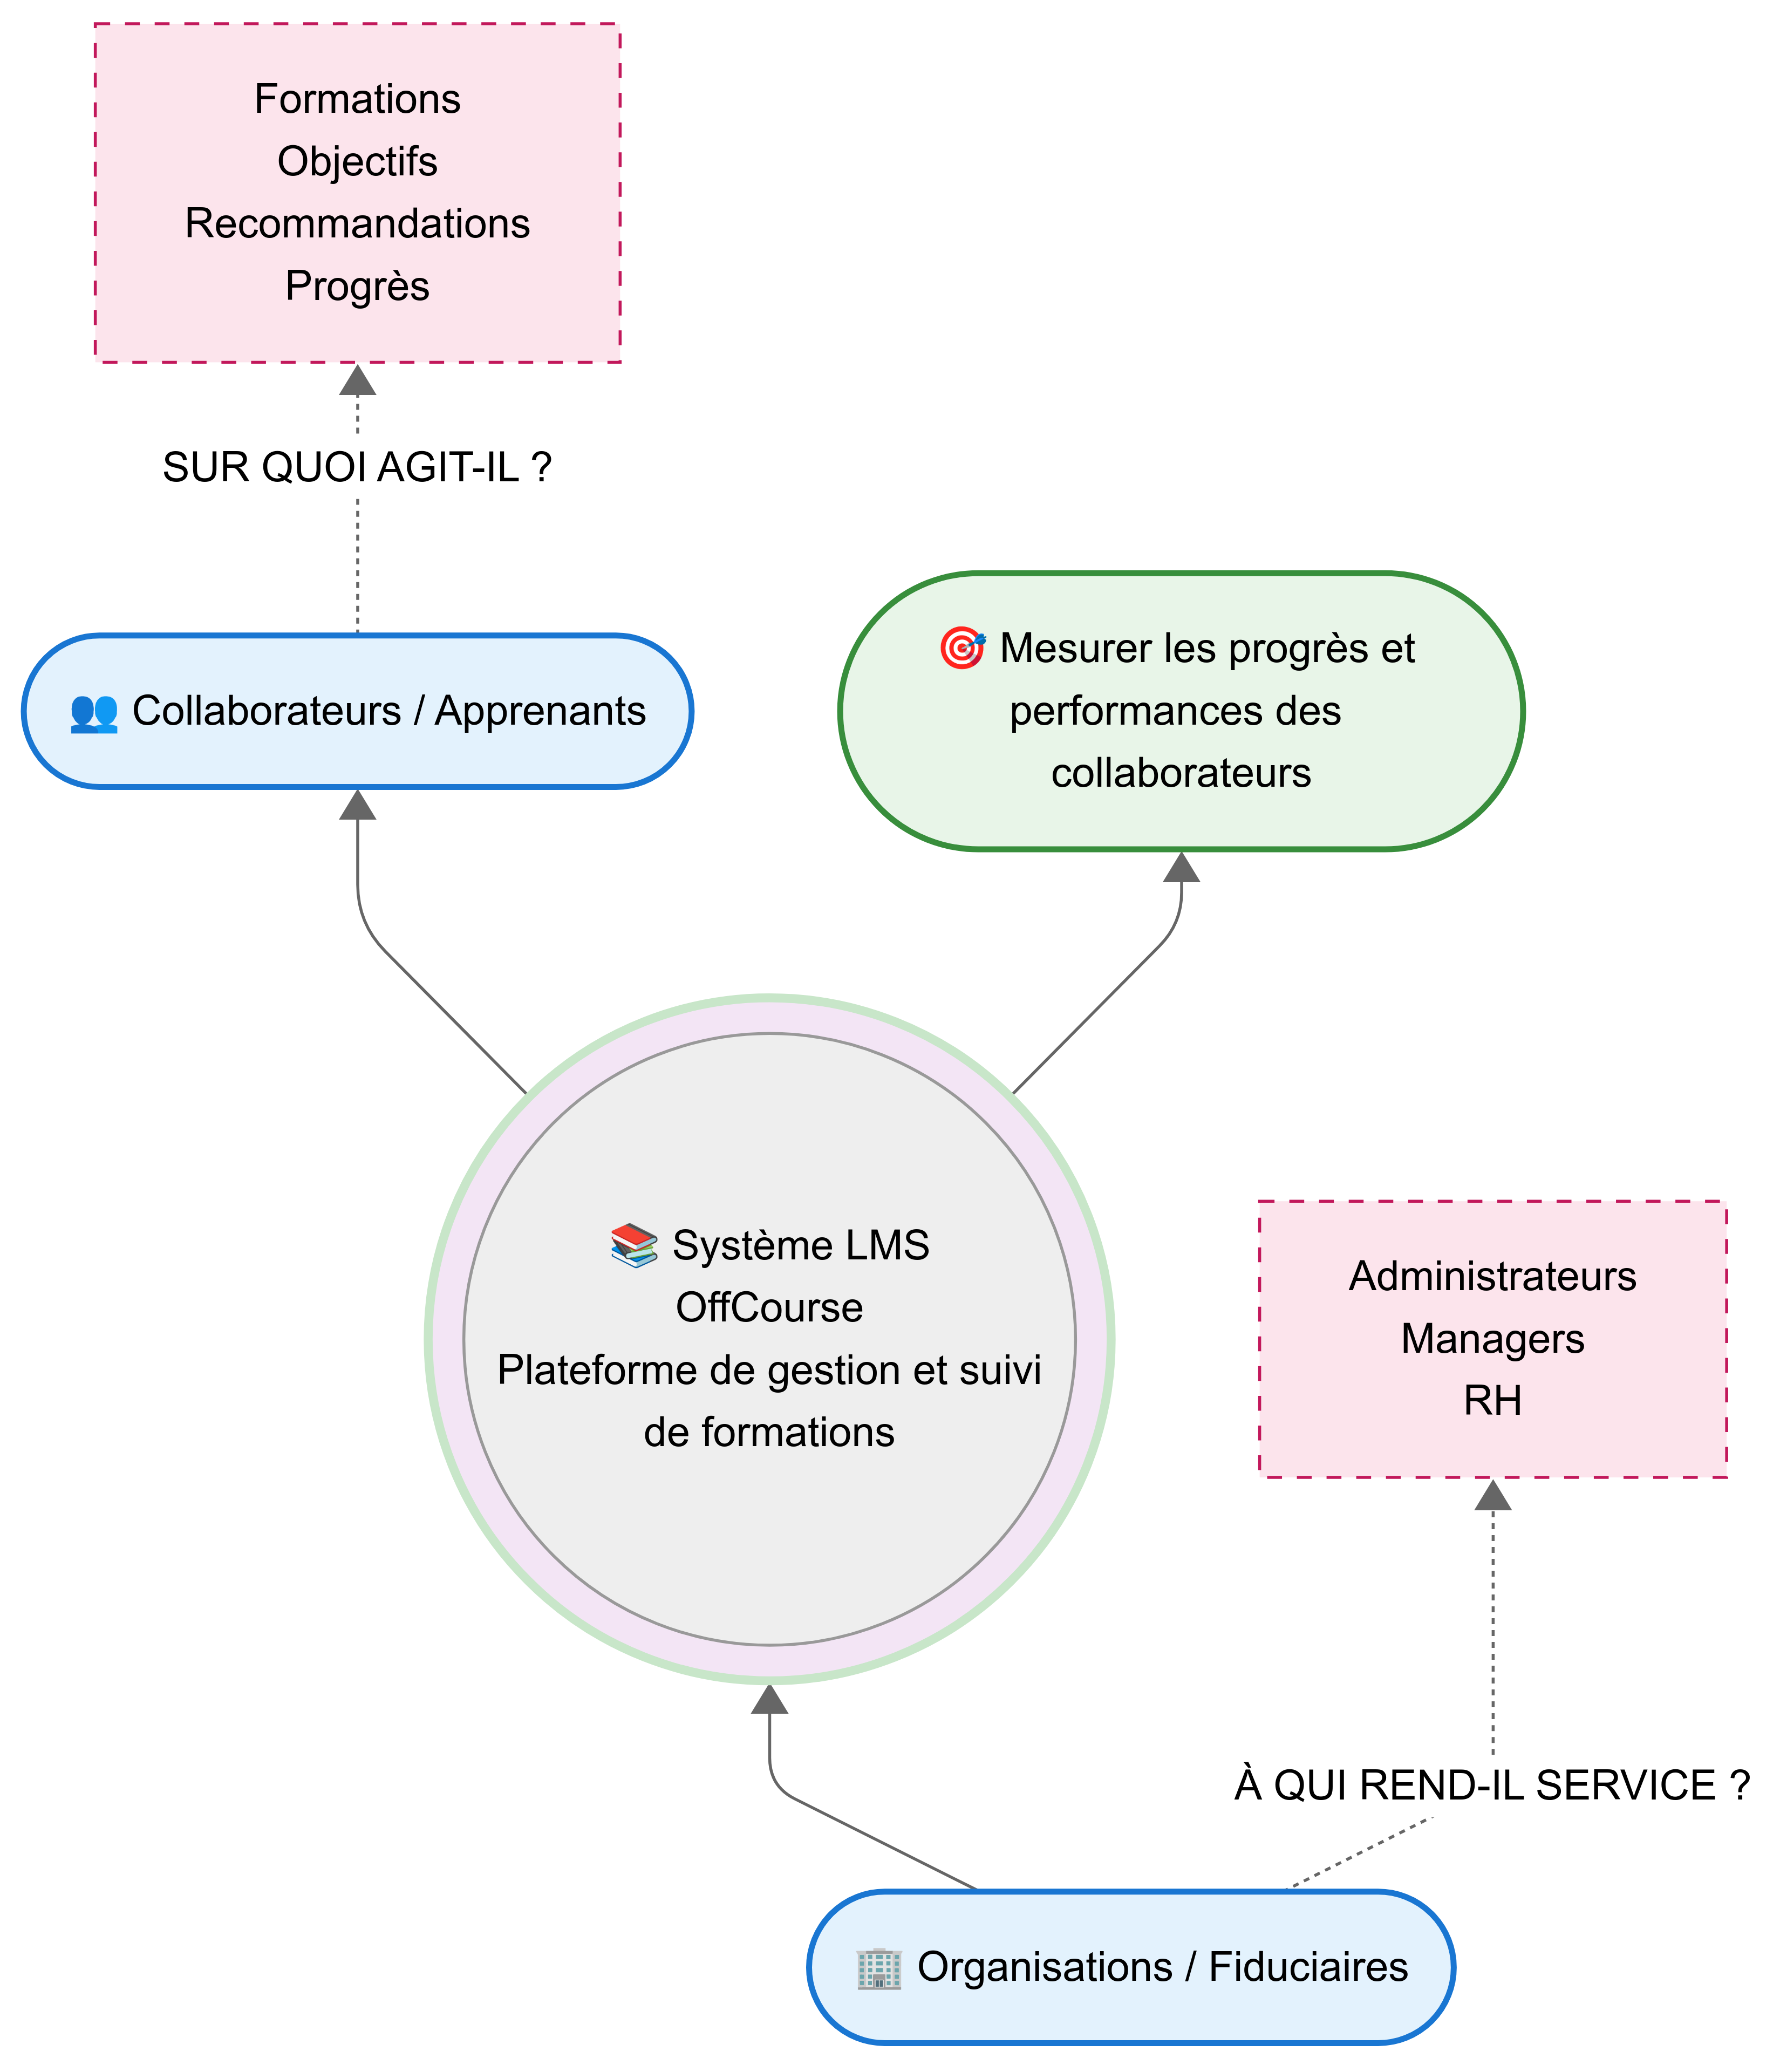
\includegraphics[width=0.85\linewidth]{beteAcorne.png}
\caption{Diagramme Bête à Cornes - System LMS OffCourse}
\end{figure}
\hfill

\vspace{10cm}
\textbf{Analyse du diagramme :}
\begin{itemize}
    \item \textbf{À qui rend-il service ?} Organisations/Fiduciaires, Collaborateurs/Apprenants, Administrateurs/Managers/RH
    \item \textbf{Sur quoi agit-il ?} Formations, Objectifs, Recommandations, Progrès (gestion des trimestres, suivi des objectifs, recommandations de formations)
    \item \textbf{Dans quel but ?} Optimiser la gestion des formations et le développement des compétences au sein des organisations
\end{itemize}

\subsection{Diagrammes de cas d'utilisation}

Les diagrammes de cas d'utilisation permettent de représenter les fonctionnalités du système du point de vue des utilisateurs. Ils offrent un premier pas pour comprendre les
interactions entre le système et ses différents acteurs. En effet, ceux-ci permettent de délimiter le
système en un ensemble de besoins des utilisateurs.
\subsubsection{Cas d'utilisation - Application OffCourse}

Ce diagramme de cas d'utilisation modélise les interactions entre les différents types d'utilisateurs et le système de gestion des formations OffCourse. Il illustre la hiérarchie des acteurs et met en évidence les relations UML essentielles (héritage, inclusion, extension) qui structurent le système.

\begin{figure}[ht!]
\centering
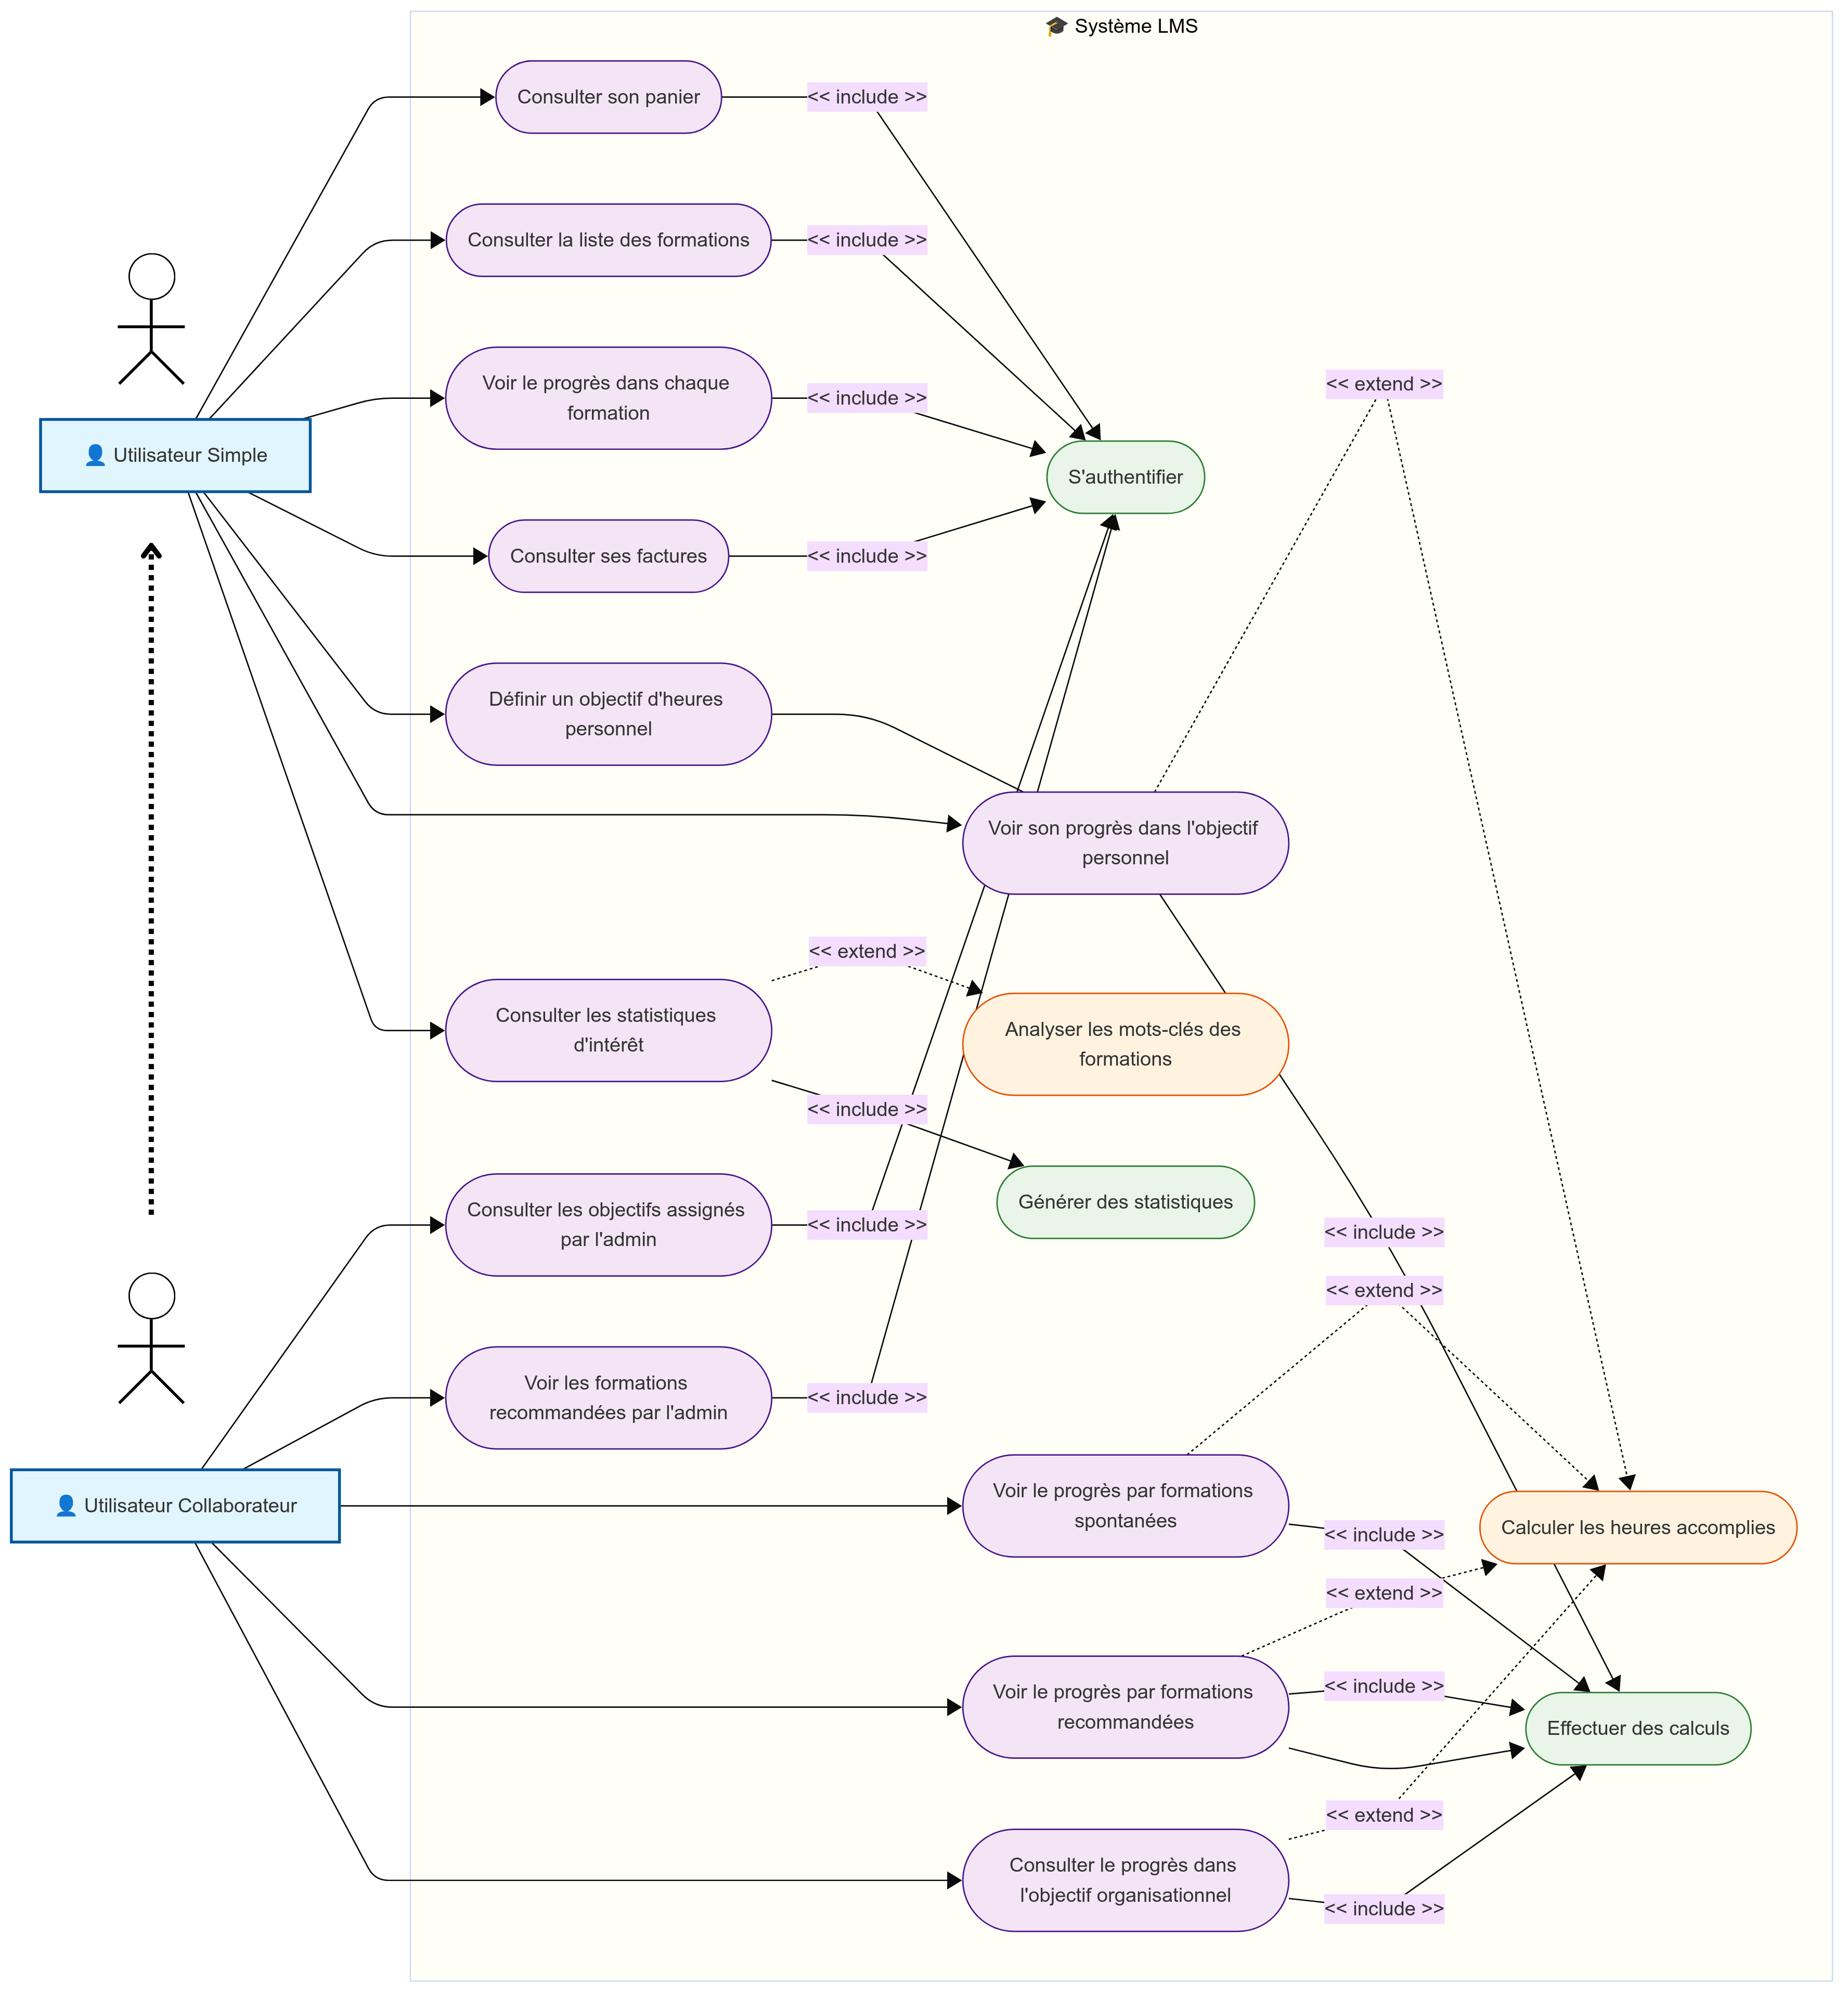
\includegraphics[width=0.85\linewidth]{useCaseoFFcourse.png}
\caption{Diagramme de cas d'utilisation - Gestion des formations OffCourse}
\end{figure}

\textbf{Architecture du système :}

Le diagramme présente une architecture hiérarchique où l'Utilisateur Collaborateur hérite de toutes les fonctionnalités de l'Utilisateur Simple, illustrant ainsi le principe de spécialisation progressive des rôles.

\textbf{Fonctionnalités par acteur :}

\textit{Utilisateur Simple :}
\begin{itemize}
    \item \textbf{Gestion des formations :} Consulter le catalogue des formations disponibles et suivre sa progression dans chaque formation
    \item \textbf{Gestion commerciale :} Consulter son panier d'achat et accéder à l'historique de ses factures
    \item \textbf{Objectifs personnels :} Définir des objectifs d'heures de formation personnalisés et suivre leur réalisation
    \item \textbf{Analyse statistique :} Consulter ses statistiques d'intérêt avec possibilité d'analyse des mots-clés des formations (relation d'extension)
\end{itemize}

\textit{Utilisateur Collaborateur} (hérite de toutes les fonctionnalités de l'Utilisateur Simple) :
\begin{itemize}
    \item \textbf{Gestion organisationnelle :} Consulter les objectifs assignés par l'administrateur de son organisation
    \item \textbf{Formations recommandées :} Accéder aux formations spécifiquement recommandées par l'administration
    \item \textbf{Suivi dual :} Suivre simultanément son progrès dans l'objectif organisationnel et ses formations spontanées
    \item \textbf{Reporting avancé :} Visualiser distinctement le progrès par formations recommandées et formations choisies spontanément
\end{itemize}

\textbf{Relations UML implémentées :}

\begin{itemize}
    \item \textbf{Héritage :} L'Utilisateur Collaborateur hérite des capacités de l'Utilisateur Simple
    \item \textbf{Inclusion (<<include>>) :} Tous les cas d'utilisation incluent l'authentification, les calculs de progression incluent des fonctions de calcul automatique
    \item \textbf{Extension (<<extend>>) :} L'analyse des mots-clés étend optionnellement la consultation des statistiques
    \item \textbf{Associations :} Relations directes entre la définition d'objectifs et leur suivi
\end{itemize}

Cette modélisation garantit une séparation claire des responsabilités tout en permettant une évolutivité du système vers des rôles plus spécialisés.
\hfill
\subsubsection{Cas d'utilisation - Interface LMS United Associate}

Ce diagramme de cas d'utilisation présente l'architecture fonctionnelle complète du système LMS (Learning Management System) de l'application United Associate. Il illustre les interactions entre les différents acteurs et les fonctionnalités disponibles selon leurs rôles et permissions.

\begin{figure}[htbp]
\hspace{2cm}
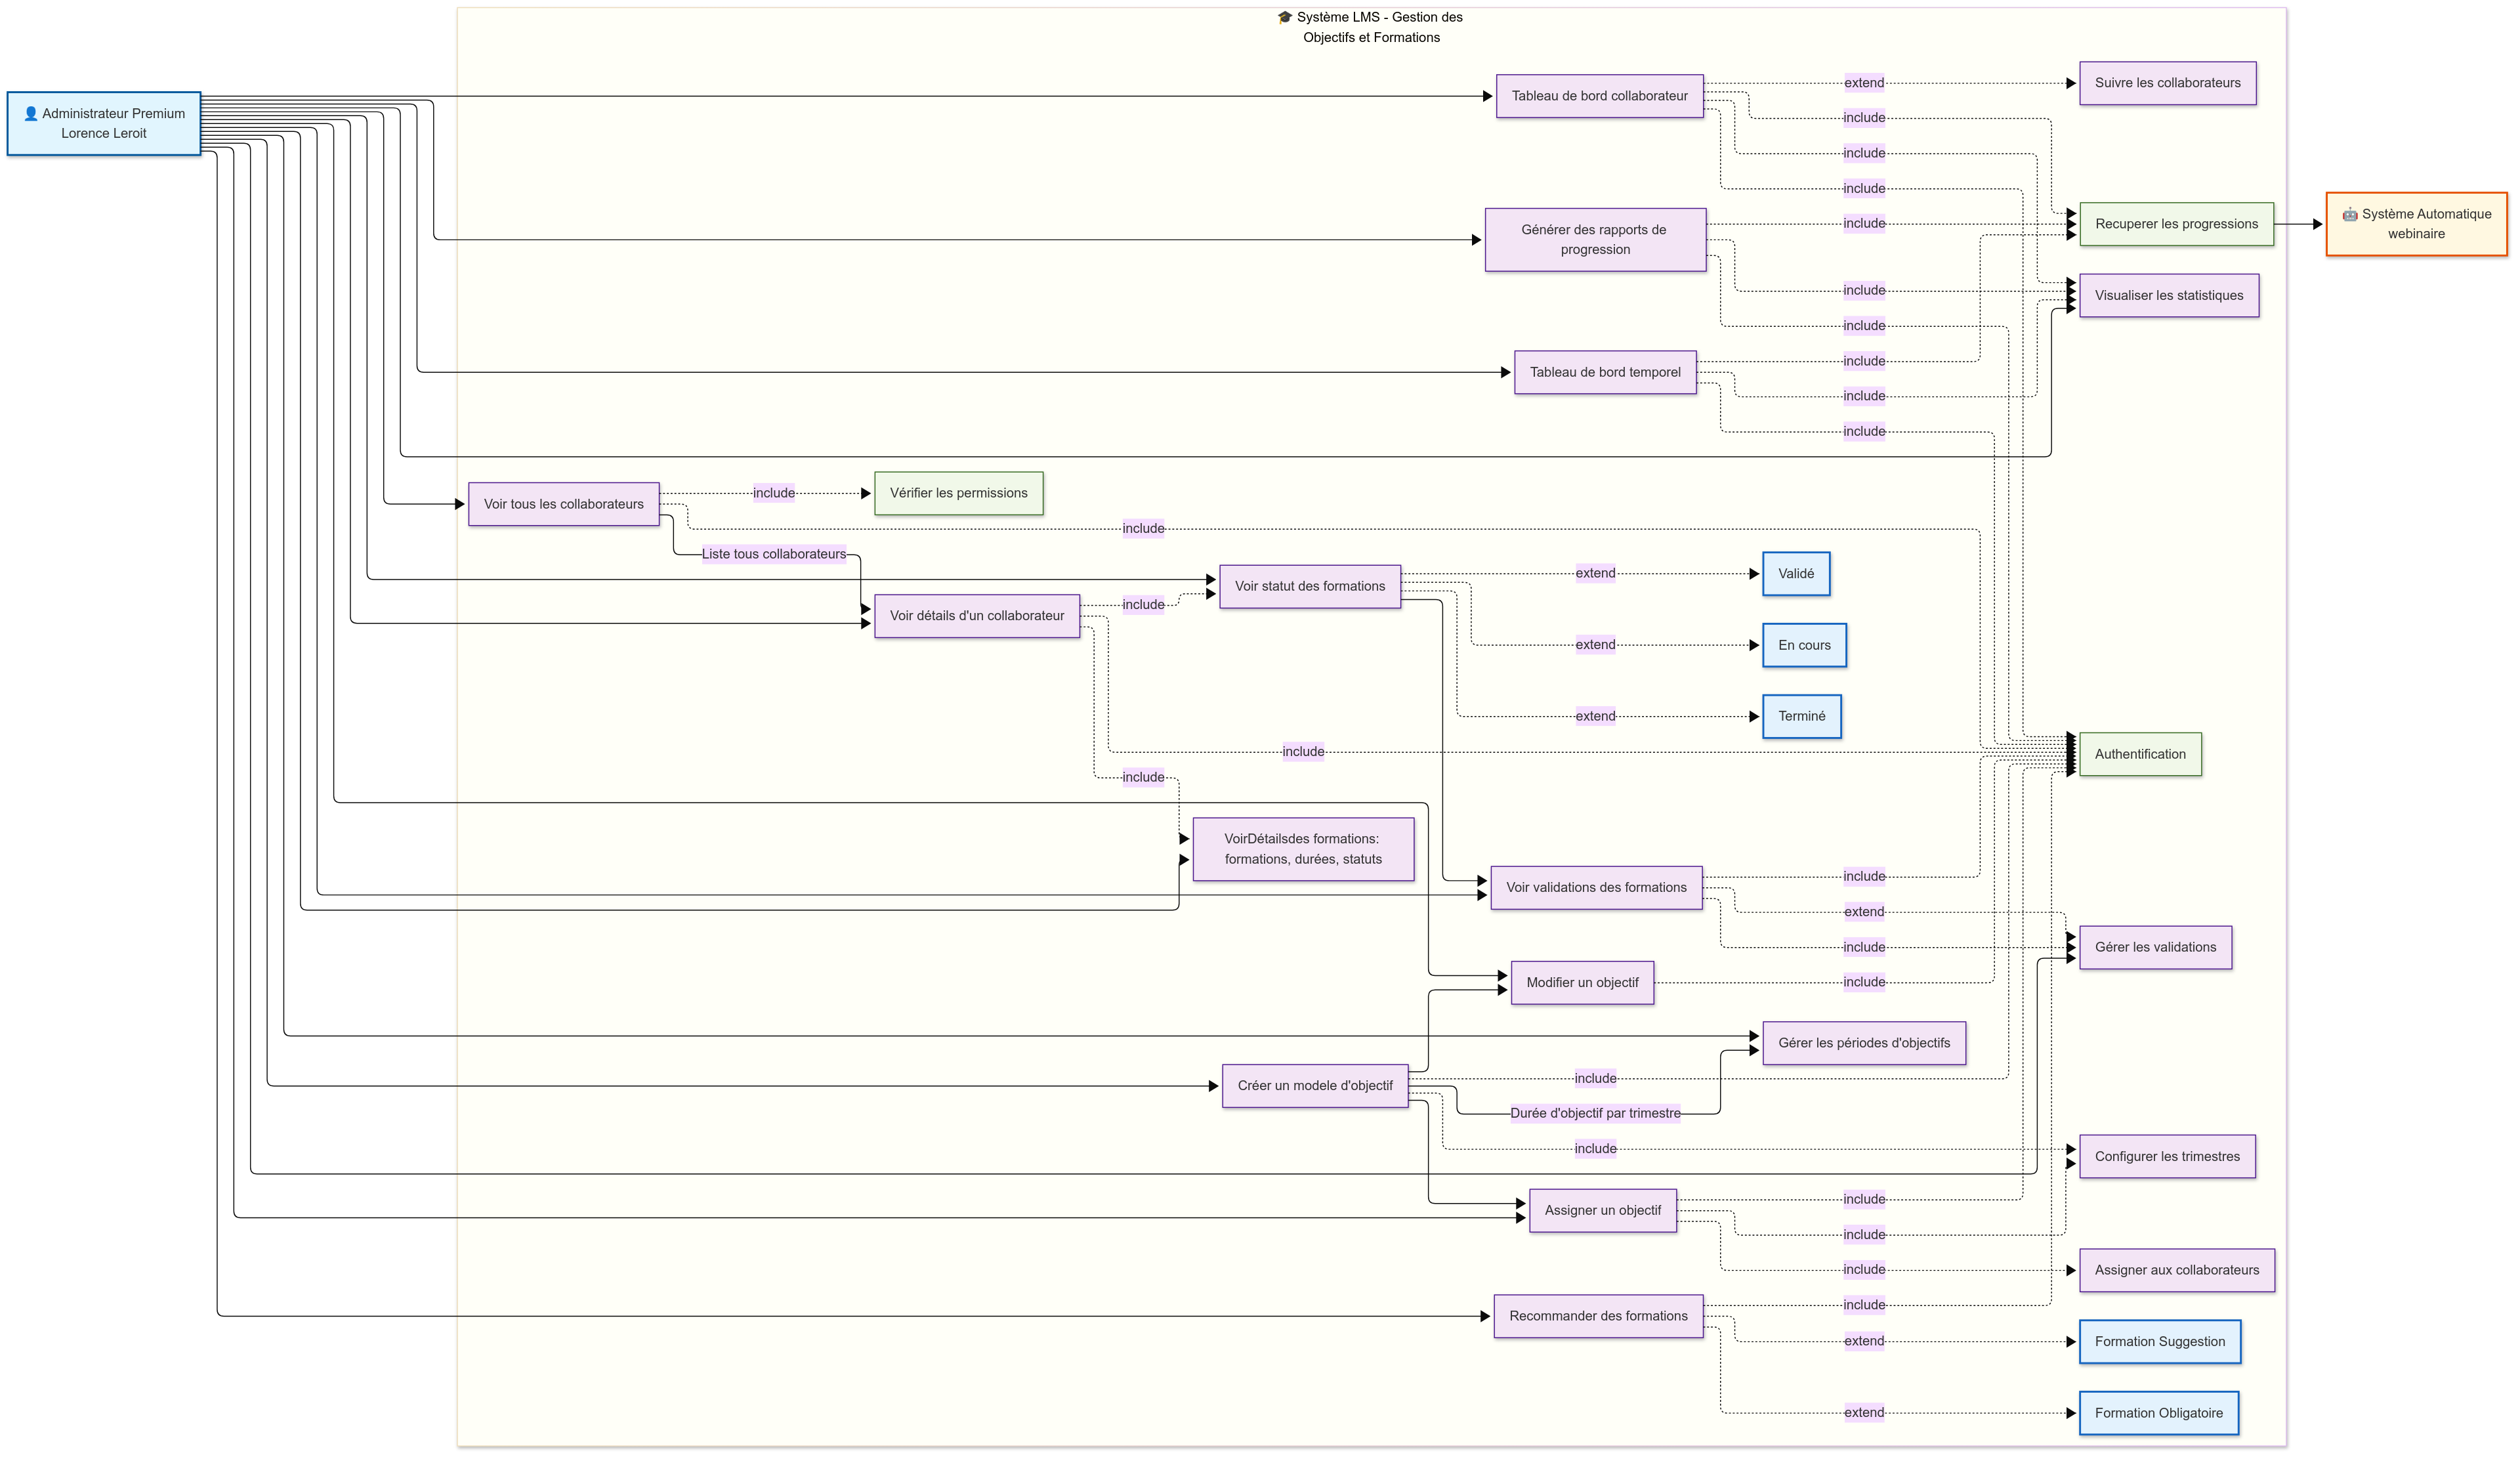
\includegraphics[width=1.25\linewidth, right]{useCaseLMS.png}
\caption{Diagramme de cas d'utilisation - Interface LMS United Associate}
\end{figure}

\paragraph{Acteurs du système :}
\begin{itemize}
    \item \textbf{Collaborateurs} : Utilisateurs finaux qui consultent leurs objectifs, suivent leurs formations et accèdent à leur tableau de bord personnel
    \item \textbf{Système Automatique} : Gère les calculs de progression, les notifications et les mises à jour automatiques
\end{itemize}

\paragraph{Fonctionnalités principales :}

\textbf{Gestion des objectifs et périodes :}
\begin{itemize}
    \item Configuration des trimestres et périodes d'objectifs 
    \item Création et modification d'objectifs avec durées personnalisables 
    \item Assignation d'objectifs spécifiques aux collaborateurs
    \item Suivi des progressions avec calculs automatiques
\end{itemize}

\textbf{Système de formation et recommandations :}
\begin{itemize}
    \item Recommandation de formations avec deux types : \textit{Obligatoire} et \textit{Suggestion}
    \item Assignation de formations spécialisées (taxation, risk management, etc.)
    \item Suivi des statuts de formation : \textit{Terminé}, \textit{En cours}, \textit{Validé}
    \item Système de validation administrateur pour les formations complétées
\end{itemize}

\textbf{Interfaces de suivi et tableaux de bord :}
\begin{itemize}
    \item \textbf{Vue Collaborateur} : Tableau de bord personnel avec indicateurs de progression 
    \item \textbf{Vue Administrateur} : interface de gestion globale avec vue détaillée de tous les collaborateurs.
    \item Historique complet des formations par collaborateur
    \item Génération de rapports et statistiques de performance.
\end{itemize}

\textbf{Fonctionnalités administratives avancées :}
\begin{itemize}
    \item Consultation détaillée des profils collaborateurs
    \item Gestion des validations et approbations de formations.
    \item Suivi global avec compteurs 
    \item Système d'authentification et de gestion des permissions
\end{itemize}

Ce système permet une gestion complète et hiérarchisée des compétences et des formations au sein de l'organisation, avec des outils de suivi adaptés à chaque type d'utilisateur.
\subsection{Diagrammes de séquence du système}

Dans le cadre de la conception du système LMS, les diagrammes de séquence jouent un rôle essentiel en décrivant avec précision l’enchaînement temporel des messages échangés entre les acteurs externes et les différents modules internes. Ils constituent un support précieux pour comprendre, valider et communiquer la logique de fonctionnement du système tout au long de son cycle de vie.

\subsubsection{Séquence — Utilisateur OffCourse}

Le diagramme de séquence ci-après met en lumière l’ensemble des interactions qu’un utilisateur peut avoir avec la plateforme OffCourse. Il permet de visualiser, étape par étape, la manière dont les demandes de l’utilisateur sont traitées par le système et comment les modules collaborent pour assurer une expérience fluide et cohérente:


% Première partie du diagramme
\begin{figure}[ht!]
\hspace{2cm}
    \adjustbox{trim=0 {.48\height} 0 0, clip, width=1.2\linewidth, right}{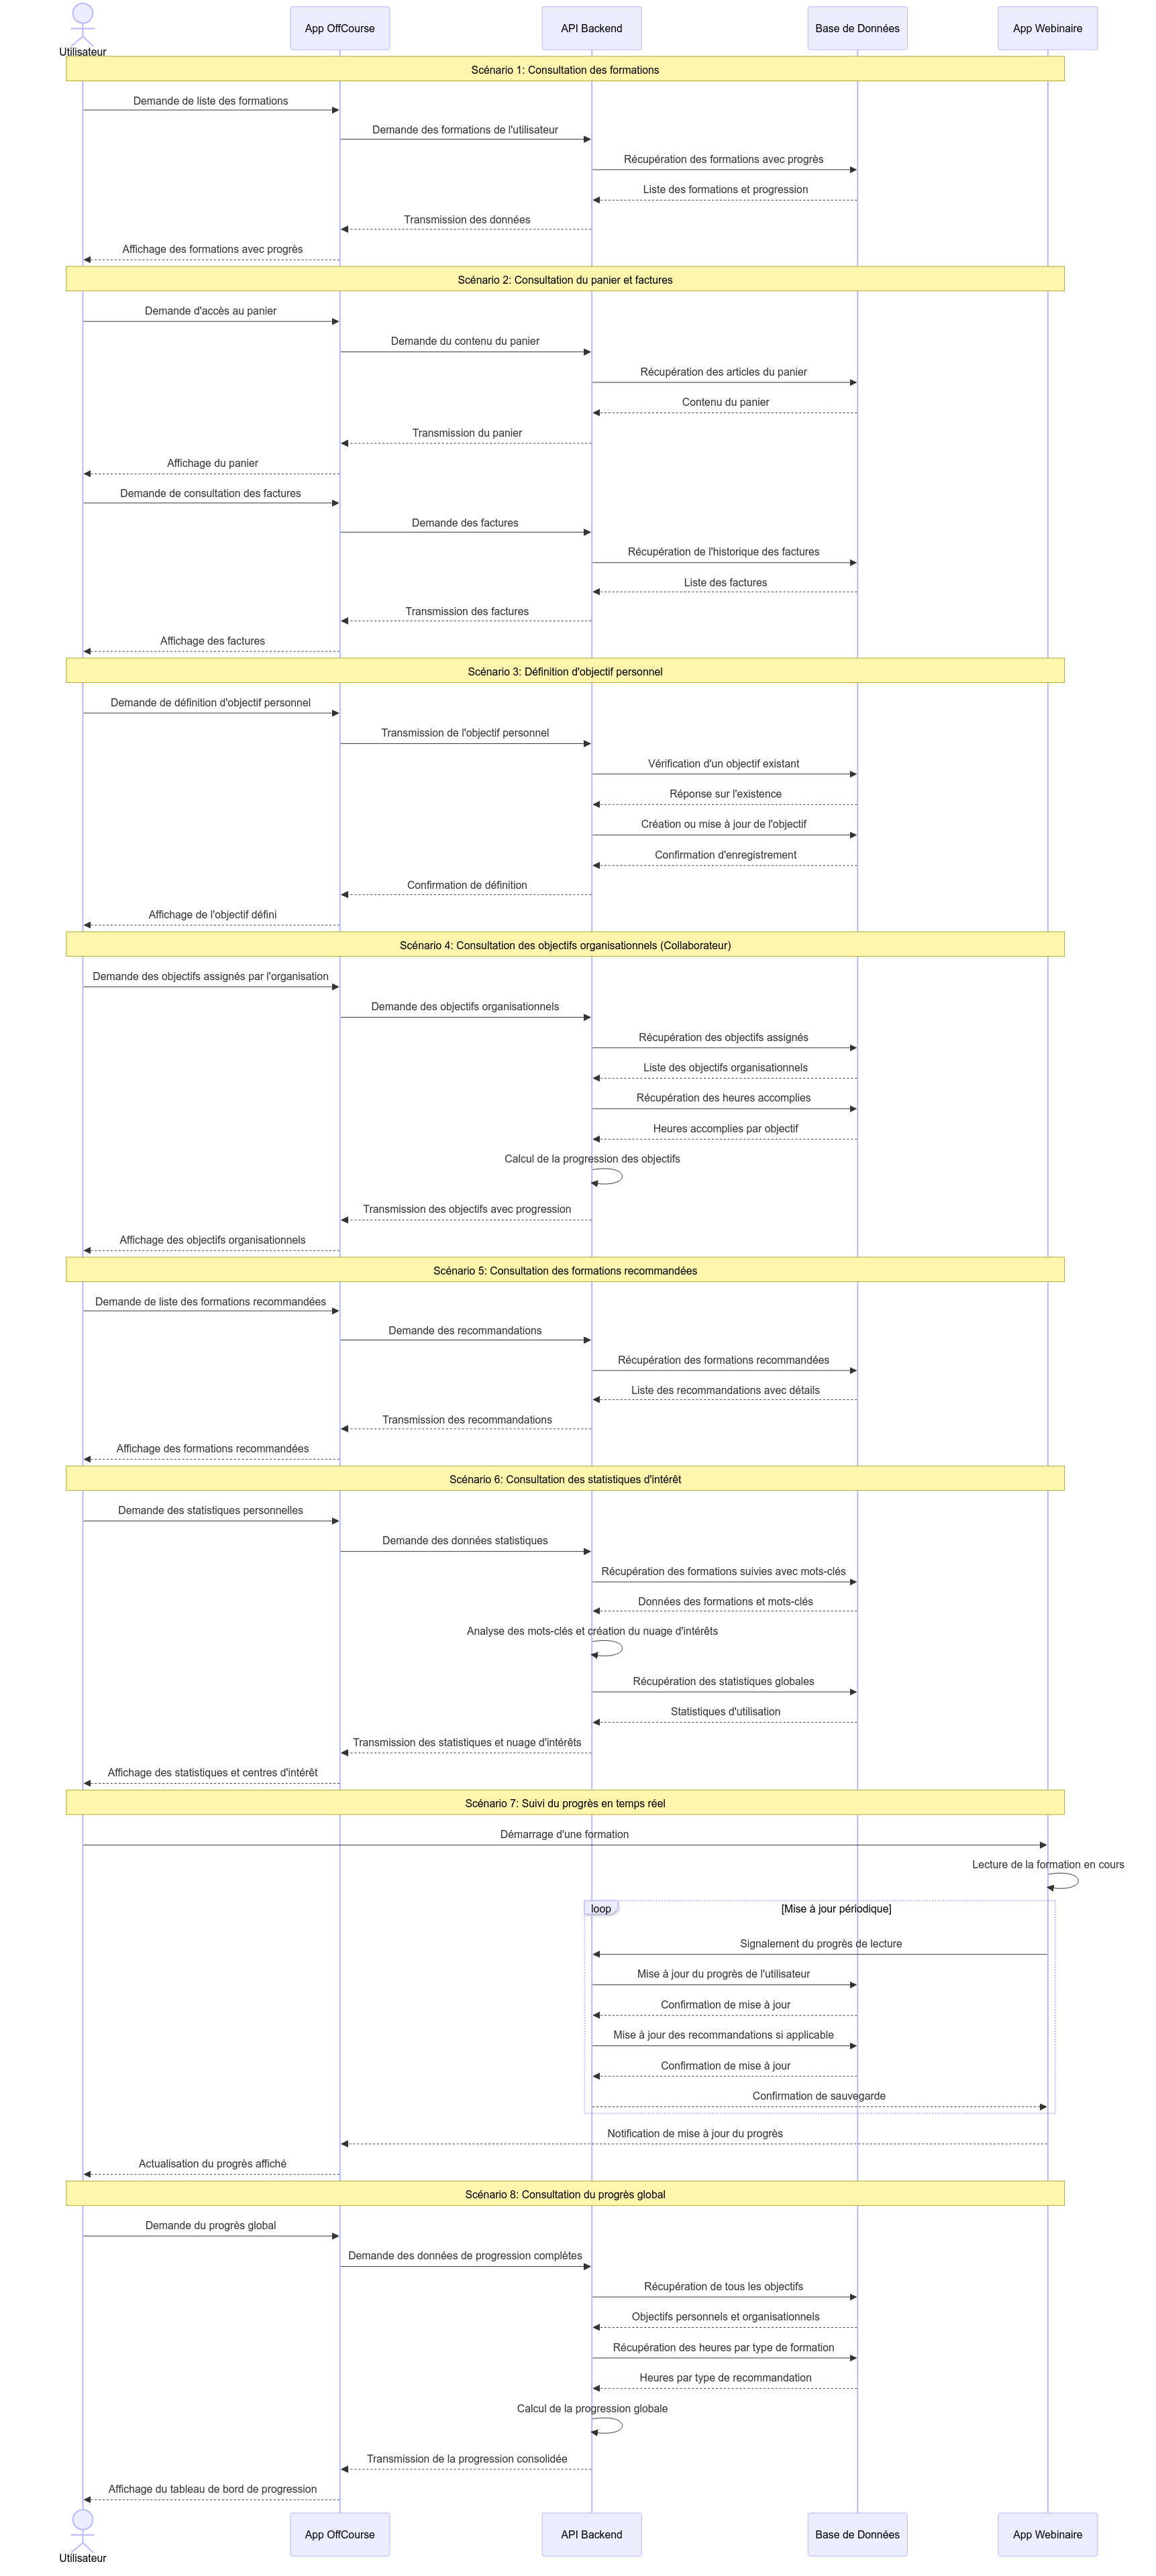
\includegraphics{sequenceLMS.png}}
    \caption{Diagramme de séquence — Interactions utilisateur OffCourse (Partie 1)}
\end{figure}

\newpage

% Deuxième partie du diagramme
\begin{figure}[ht!]
\hspace{2cm}
    \adjustbox{trim=0 0 0 {.49\height}, clip, width=1.2\linewidth, right}{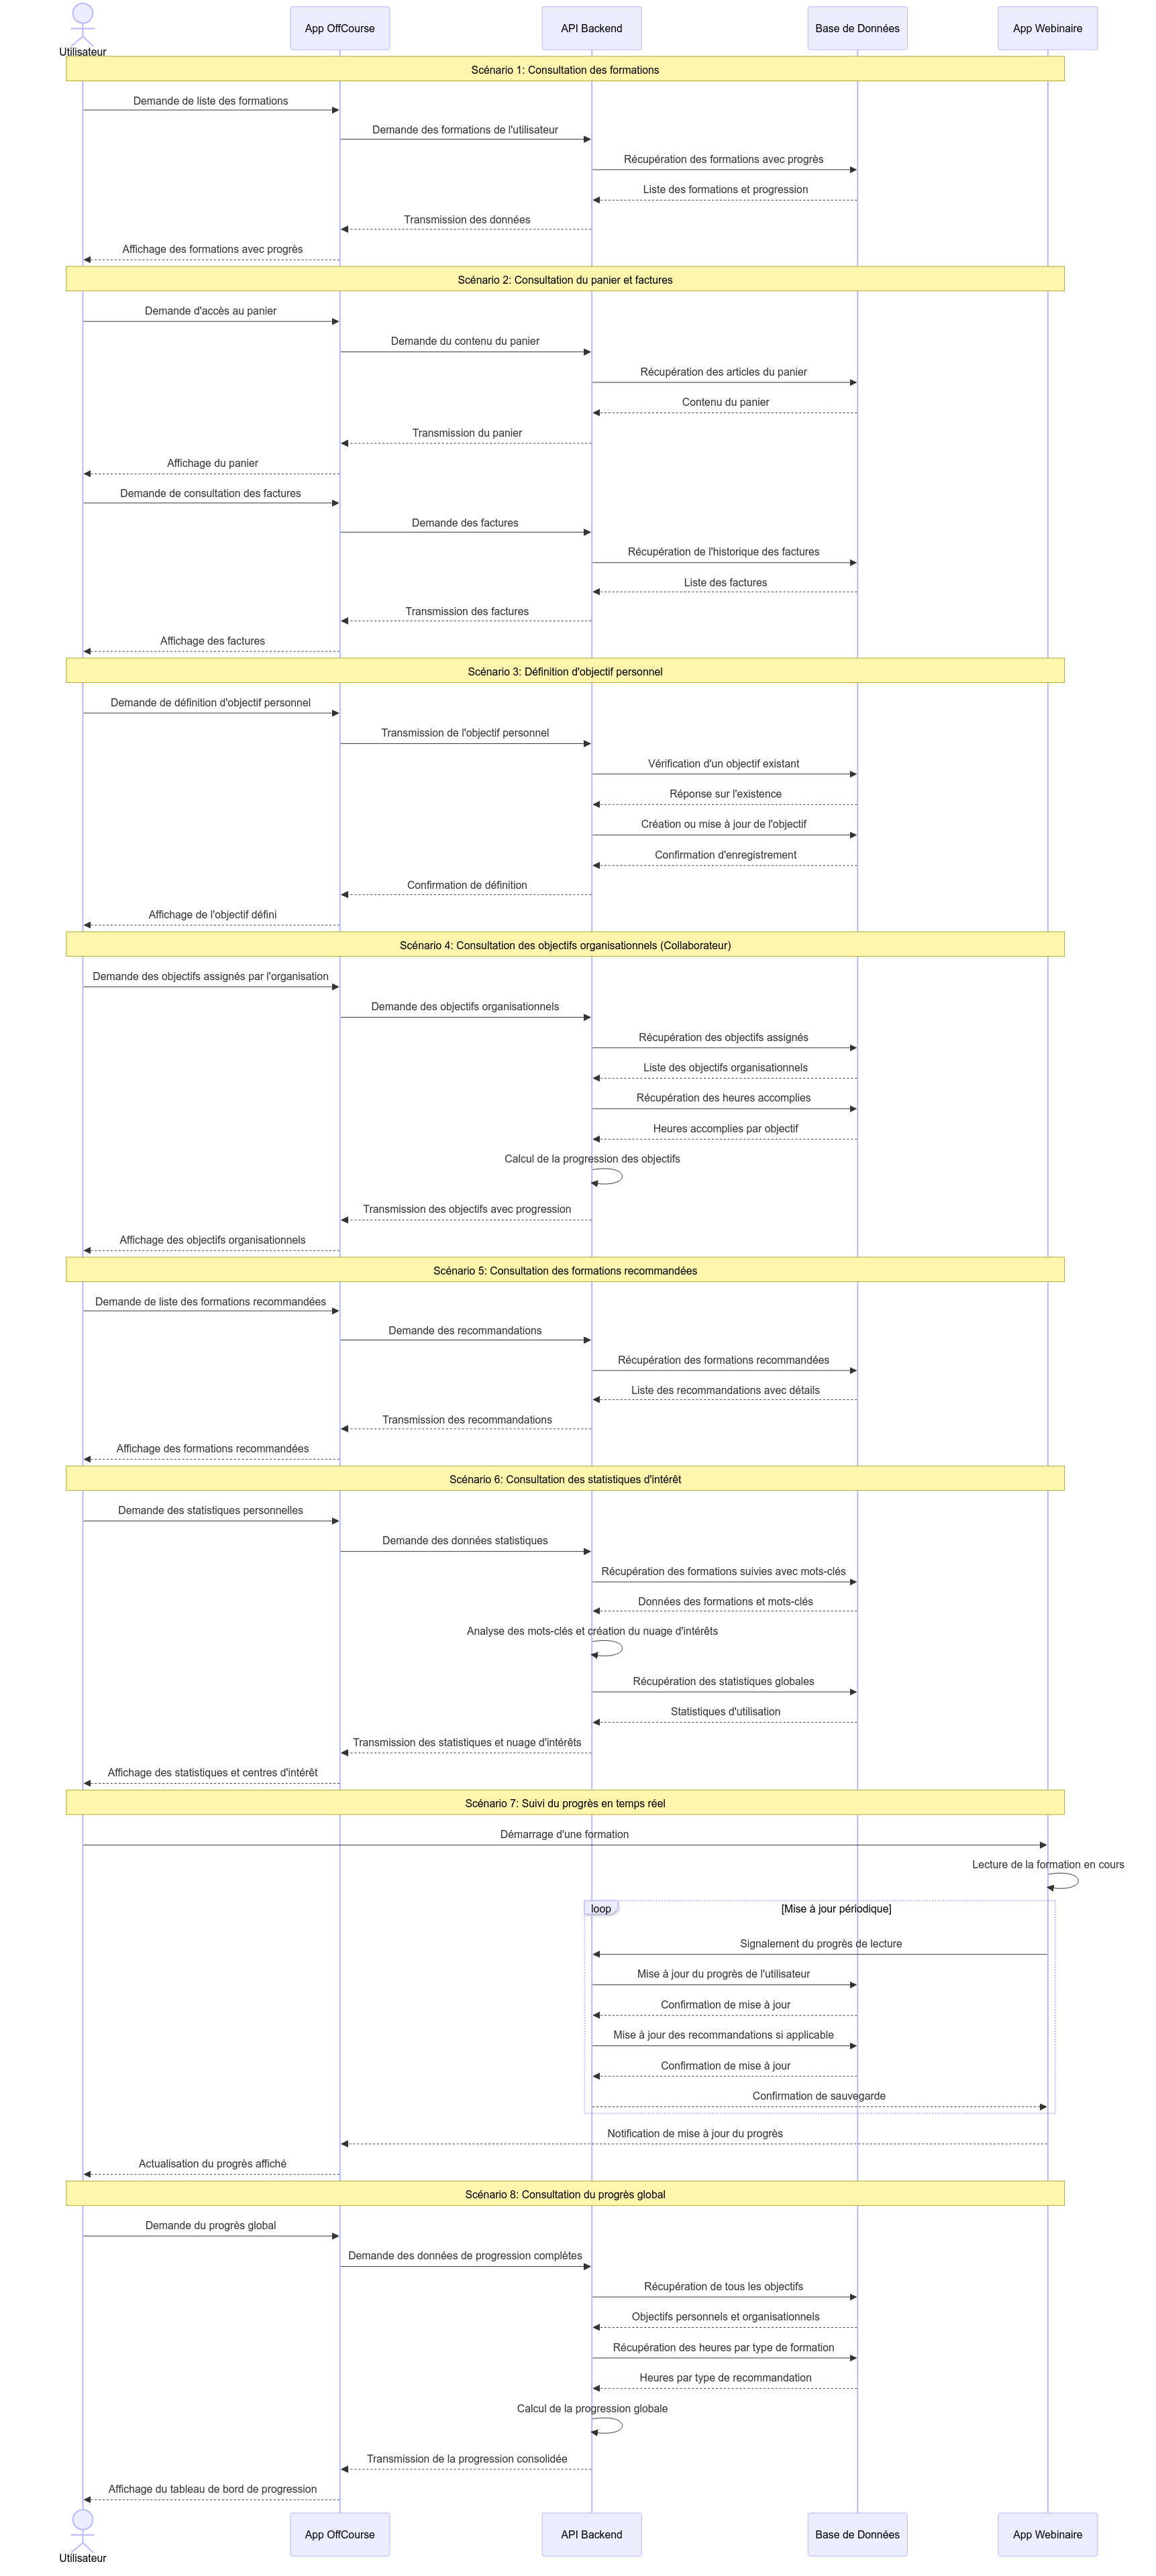
\includegraphics{sequenceLMS.png}}
    \caption{Diagramme de séquence — Interactions utilisateur OffCourse (Partie 2)}
\end{figure}

Dans ces scénarios, l’utilisateur consulte les formations mises à sa disposition, gère ses objectifs de formation à la fois individuels et organisationnels et reçoit des recommandations adaptées à ses besoins spécifiques. Le suivi de la progression est également automatisé grâce à une communication constante entre les composants internes, garantissant ainsi la mise à jour en temps réel des indicateurs de performance. De plus, ce diagramme révèle comment le système orchestre la synchronisation des données pour préserver l’intégrité et la cohérence des informations affichées à l’utilisateur.
L’étude de ce diagramme est primordiale pour vérifier la robustesse des processus de gestion des formations et des recommandations, et pour identifier d’éventuelles optimisations susceptibles d’améliorer l’efficacité globale de la plateforme.

\begin{itemize}
    \item Consultation et sélection de contenus pédagogiques adaptés.
    \item Gestion et paramétrage des objectifs de formation personnels et collectifs.
    \item Visualisation du niveau d’avancement et réception de suggestions personnalisées.
    \item Synchronisation continue entre les modules pour garantir la fiabilité des données.
\end{itemize}


\subsubsection{Séquence — Administrateur United Associate}

Le second diagramme de séquence présente de manière détaillée les principales opérations réalisées par un administrateur au sein de l’environnement LMS de United Associate. Il sert de référence pour analyser les responsabilités de gestion et de supervision confiées aux administrateurs, ainsi que pour vérifier la bonne circulation des informations entre les différents services du système.
\begin{figure}[ht!]
\hspace{1.5cm}
    \adjustbox{trim=0 {.65\height} 0 0 , clip, width=1.2\linewidth, right}
% \begin{figure}[htbp]
% \centering
{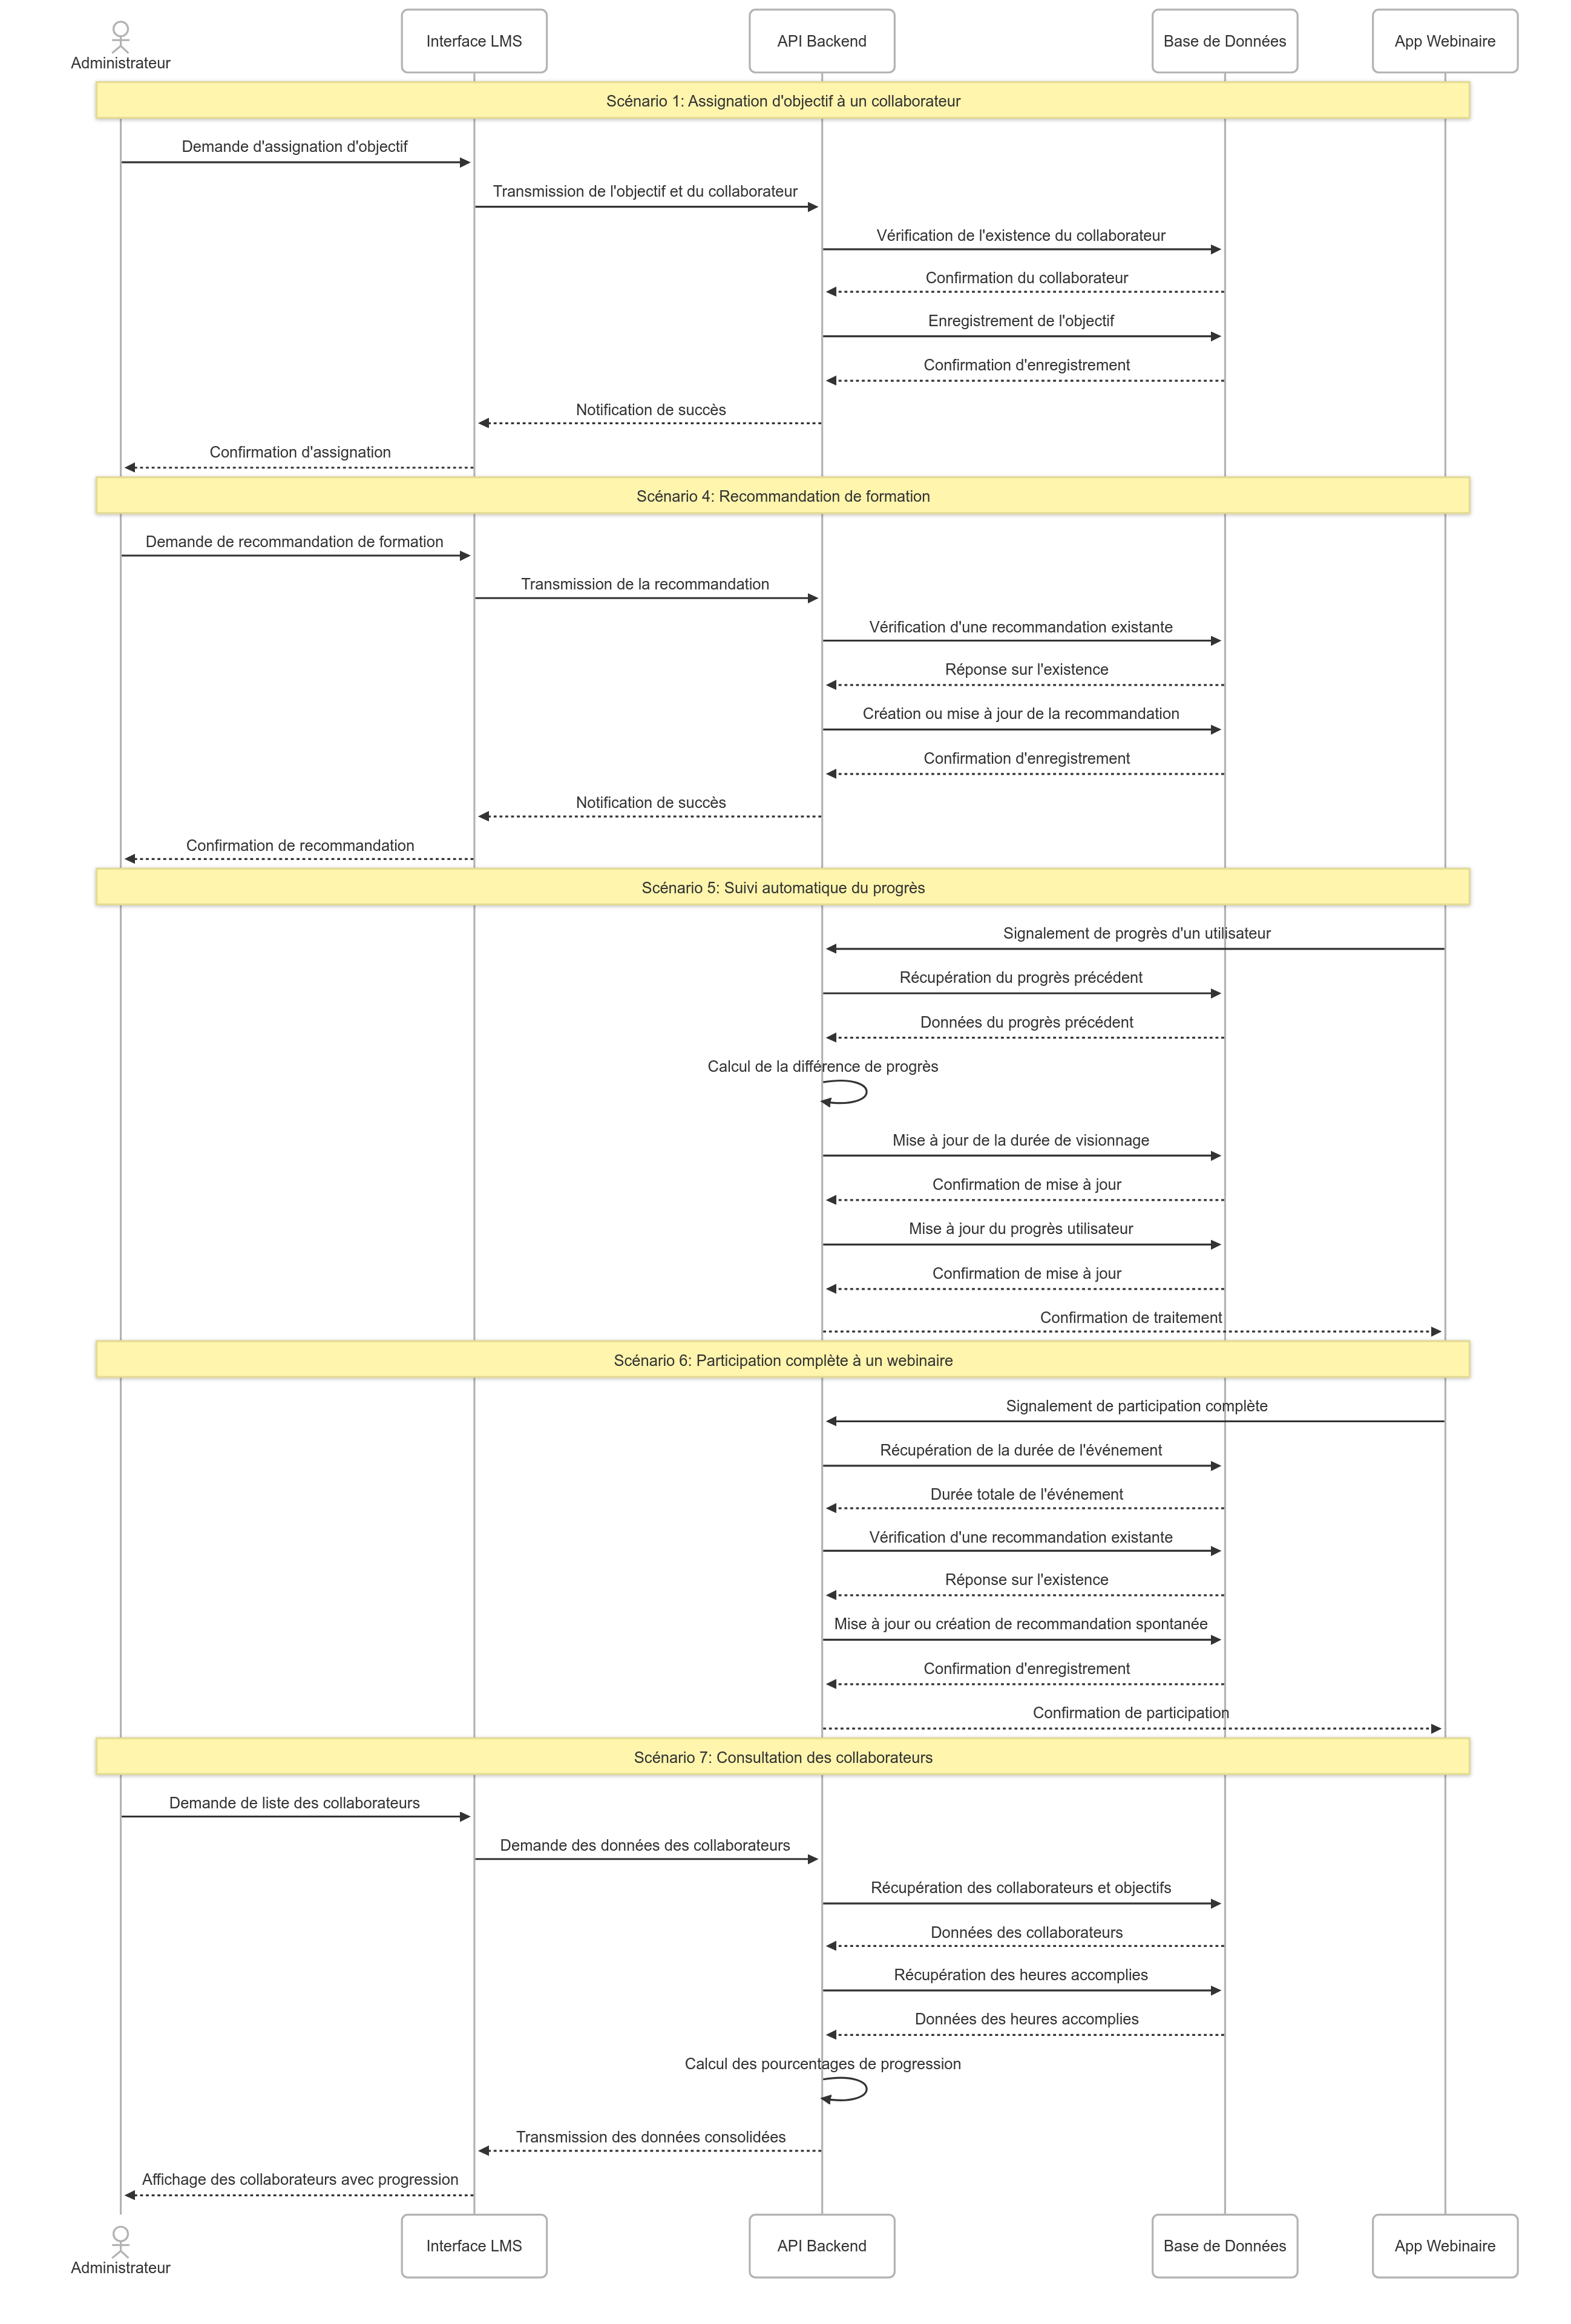
\includegraphics[width=1\linewidth]{sequenceAdmin.png}}
\caption{Diagramme de séquence — Processus administratif LMS United Associate}
\end{figure}
\begin{figure}[ht!]
\hspace{1.5cm}
    \adjustbox{trim=0 0 0 {.25\height} , clip, width=1.2\linewidth, right}
% \begin{figure}[htbp]
% \centering
{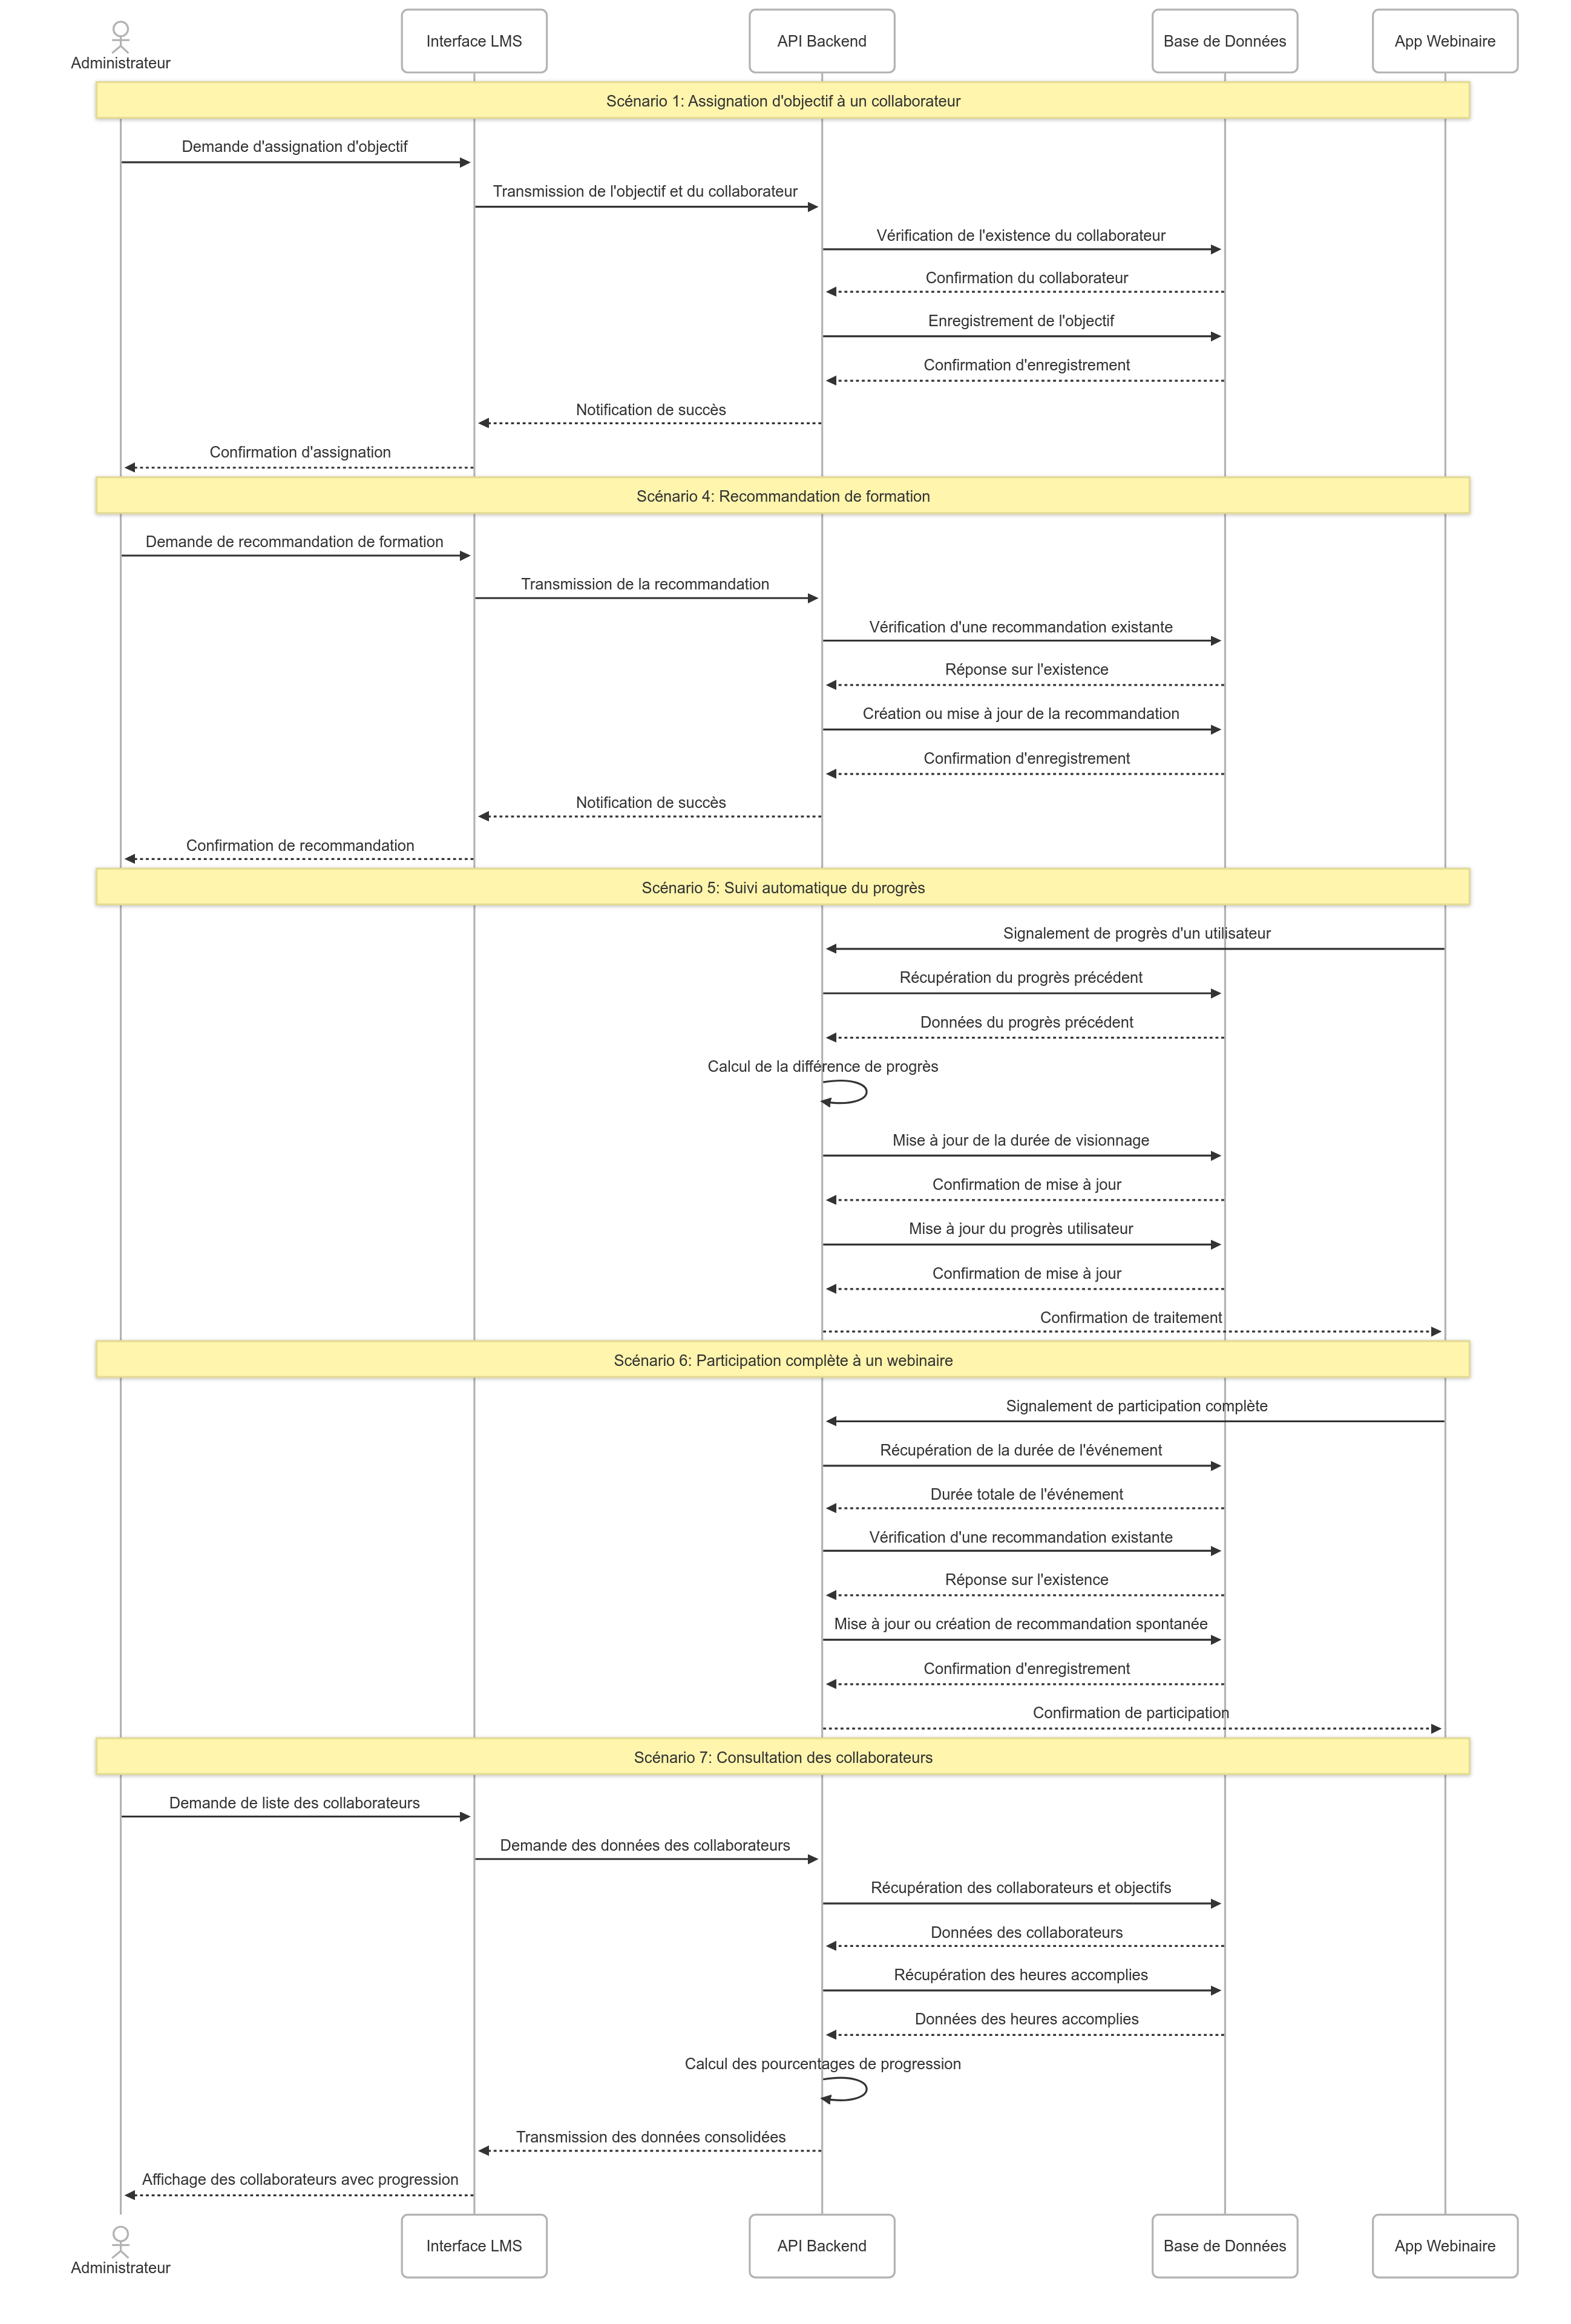
\includegraphics[width=1\linewidth]{sequenceAdmin.png}}
\caption{Diagramme de séquence — Processus administratif LMS United Associate}
\end{figure}
\\
À travers ces scénarios, l’administrateur définit les périodes de formation en créant et configurant les trimestres, puis attribue des objectifs aux collaborateurs selon les besoins pédagogiques identifiés. Il procède ensuite à la recommandation de formations spécifiques, en veillant à ce que celles-ci répondent aux exigences de montée en compétences du personnel. Le système assure en parallèle le suivi automatique de l’avancement, ce qui permet à l’administrateur de consulter des rapports à jour sans intervention manuelle. Cette automatisation réduit considérablement la charge de travail tout en renforçant la précision des données collectées.

Ce diagramme confirme que le rôle de l’administrateur est central pour maintenir l’efficacité et la pertinence du dispositif de formation continue. Il permet également d’anticiper d’éventuelles évolutions futures pour intégrer de nouvelles fonctionnalités administratives.

\begin{itemize}
    \item Définition et paramétrage des périodes trimestrielles de formation.
    \item Attribution d’objectifs spécifiques en fonction du profil des collaborateurs.
    \item Sélection et recommandation de formations ciblées.
    \item Suivi et mise à jour automatisés du niveau d’accomplissement des objectifs.
    \item Consultation et analyse des données individuelles et collectives des collaborateurs.
\end{itemize}


\subsection{Modèle du domaine}

Le modèle du domaine représente les concepts métier et leurs relations dans le contexte du système LMS.

\begin{figure}[ht!]
\hspace{2cm}
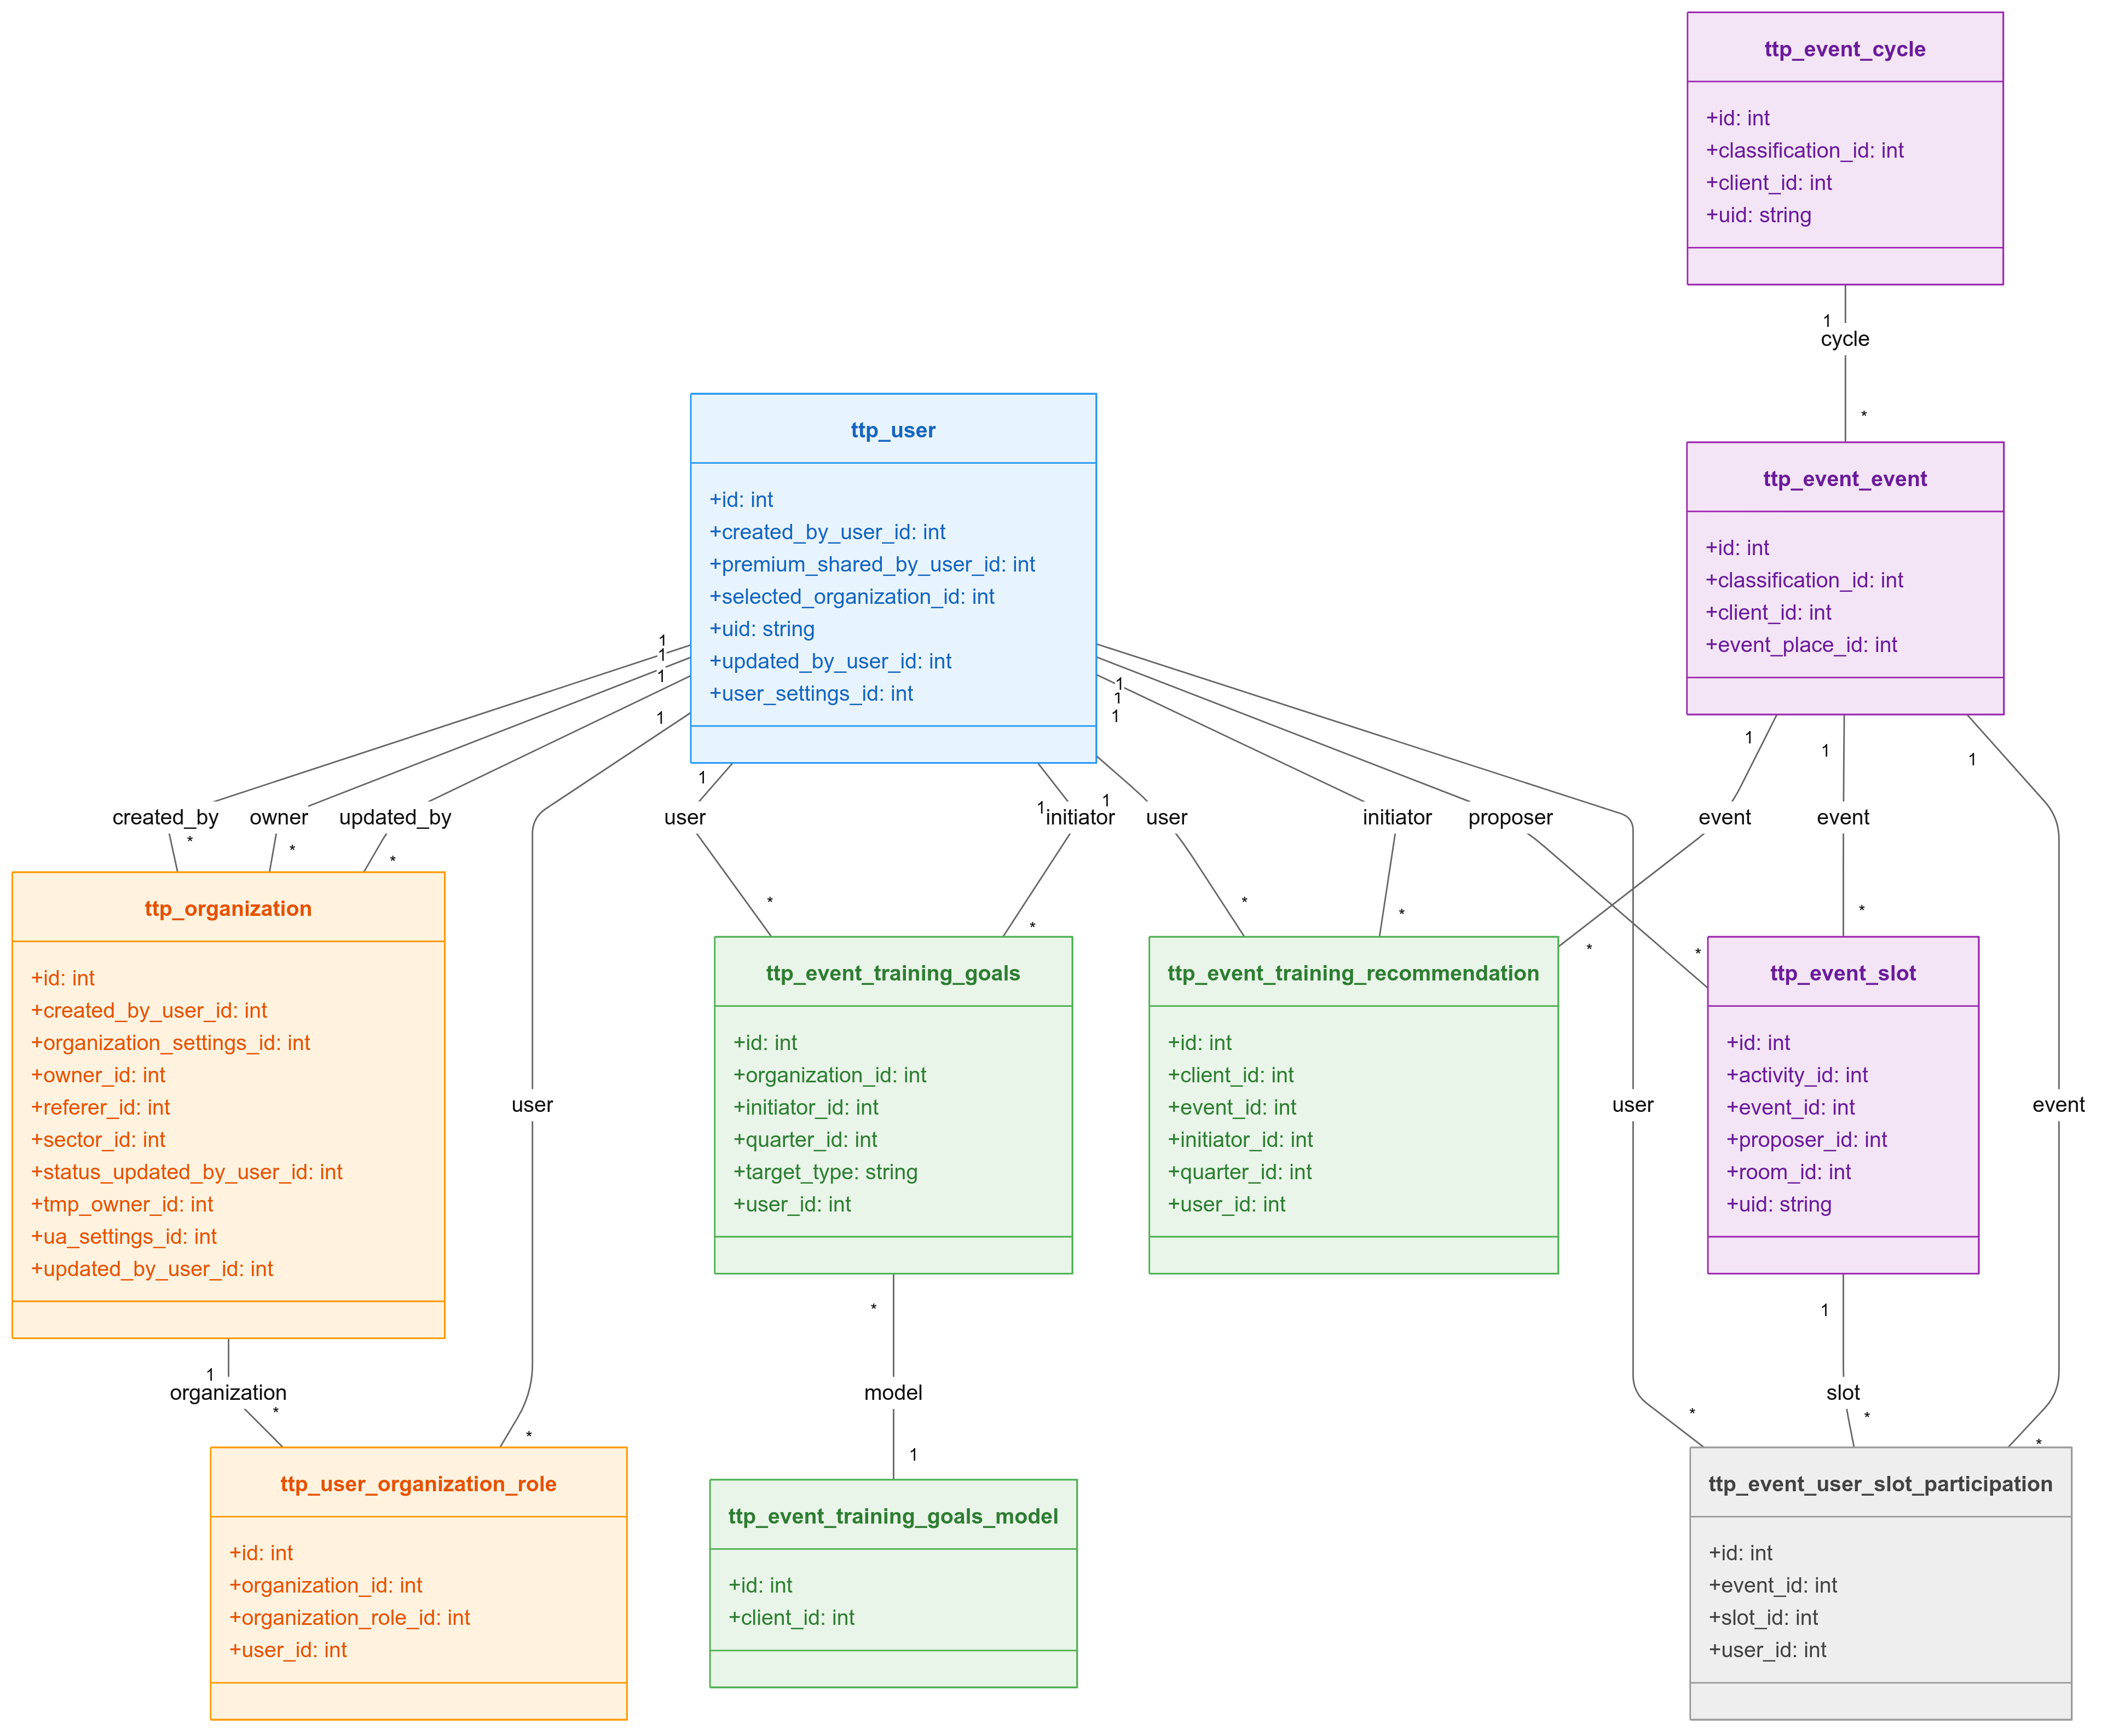
\includegraphics[width=1.2\linewidth,right]{Editor _ Mermaid Chart-2025-06-10-161411.png}
\caption{Modèle du domaine - Système LMS}
\end{figure}
\textbf{Analyse du modèle :}

Le modèle révèle une architecture centrée sur l'entité \texttt{User} qui peut jouer différents rôles selon son contexte organisationnel. Les entités principales sont :

\begin{itemize}
    \item \textbf{User} : Entité centrale représentant tous les utilisateurs du système
    \item \textbf{Organization} : Structure regroupant les collaborateurs
    \item \textbf{Role} : Définit les privilèges d'accès (official, admin)
    \item \textbf{Quarter} : Période temporelle pour l'organisation des formations
    \item \textbf{TrainingGoal} : Objectifs de formation avec cibles horaires
    \item \textbf{Recommendation} : Suggestions de formations avec typologie
    \item \textbf{Event} : Formations et événements disponibles
    \item \textbf{UserSlotParticipation} : Suivi de la participation et du progrès
\end{itemize}

Les relations entre ces entités permettent de gérer la complexité des interactions organisationnelles tout en maintenant la flexibilité nécessaire pour les utilisateurs individuels.

\section{Conclusion}

Ce chapitre d'analyse et de conception a permis d'établir une base solide pour le développement du système LMS. L'utilisation d'UML nous a fourni un langage commun pour exprimer les besoins et modéliser l'architecture du système.

Les principaux résultats de cette phase d'analyse sont :

\begin{itemize}
    \item \textbf{Identification claire des acteurs} et de leurs besoins spécifiques
    \item \textbf{Modélisation complète des fonctionnalités} requises pour chaque type d'utilisateur
    \item \textbf{Architecture logique cohérente} supportant les besoins organisationnels et individuels
    \item \textbf{Spécifications détaillées} des interactions système-utilisateur
    \item \textbf{Modèle de données} robuste pour supporter l'évolutivité du système
\end{itemize}

Cette analyse constitue le fondement technique sur lequel s'appuiera la phase de développement. Elle garantit que le système répondra aux attentes des utilisateurs tout en respectant les contraintes de performance, sécurité et maintenabilité identifiées.

Le chapitre suivant présentera les choix technologiques et l'architecture technique détaillée du système, en s'appuyant sur les spécifications définies dans cette phase d'analyse.
\chapter{Étude technique}
\label{chap:technique}
Ce chapitre est consacré à l'étude technique réalisée pour la mise en œuvre du projet. En
abordant les besoins techniques, la définition de l'architecture technique du système, et en
présentant par la suite les technologies et les outils utilisés dans la phase de réalisation. Et en
clôturant par l'illustration des environnements matériels et logiciels utilisés dans le projet ainsi
que les outils définis pour supporter la méthodologie de travail.

%------------------------------------------------------------
\section{Architecture du projet}
Dans le contexte du développement logiciel, l'architecture d'un projet se réfère à la structure et à
l'organisation des principaux composants du système, ainsi qu'à la manière dont ils interagissent
entre eux. Elle englobe divers aspects, tels que la stratégie commerciale, les attributs de qualité,
la dynamique humaine, la conception et l'environnement informatique.

\subsection{Architecture physique}

L'architecture technique du système LMS repose sur une infrastructure moderne et scalable, conçue pour supporter les exigences des fiduciaires belges. Notre solution combine robustesse et flexibilité grâce aux composants suivants :

\begin{table}[htbp]
\centering
\begin{tabular}{|p{3cm}|p{10cm}|}
\hline
\textbf{Composant} & \textbf{Valeur ajoutée} \\ \hline
\textbf{Git} & Versionnement précis avec historique complet des évolutions \\ \hline
\textbf{GitHub Actions} & Automatisation des tests et déploiements après chaque modification \\ \hline
\textbf{PHP-FPM 8.2} & Exécution performante du code métier avec gestion optimisée des ressources \\ \hline
\textbf{Nginx} & Serveur web haute performance avec gestion intelligente du cache \\ \hline
\textbf{MySQL 8} & Stockage relationnel des données avec transactions ACID \\ \hline
\end{tabular}
\end{table}

\begin{figure}[htbp]
\centering
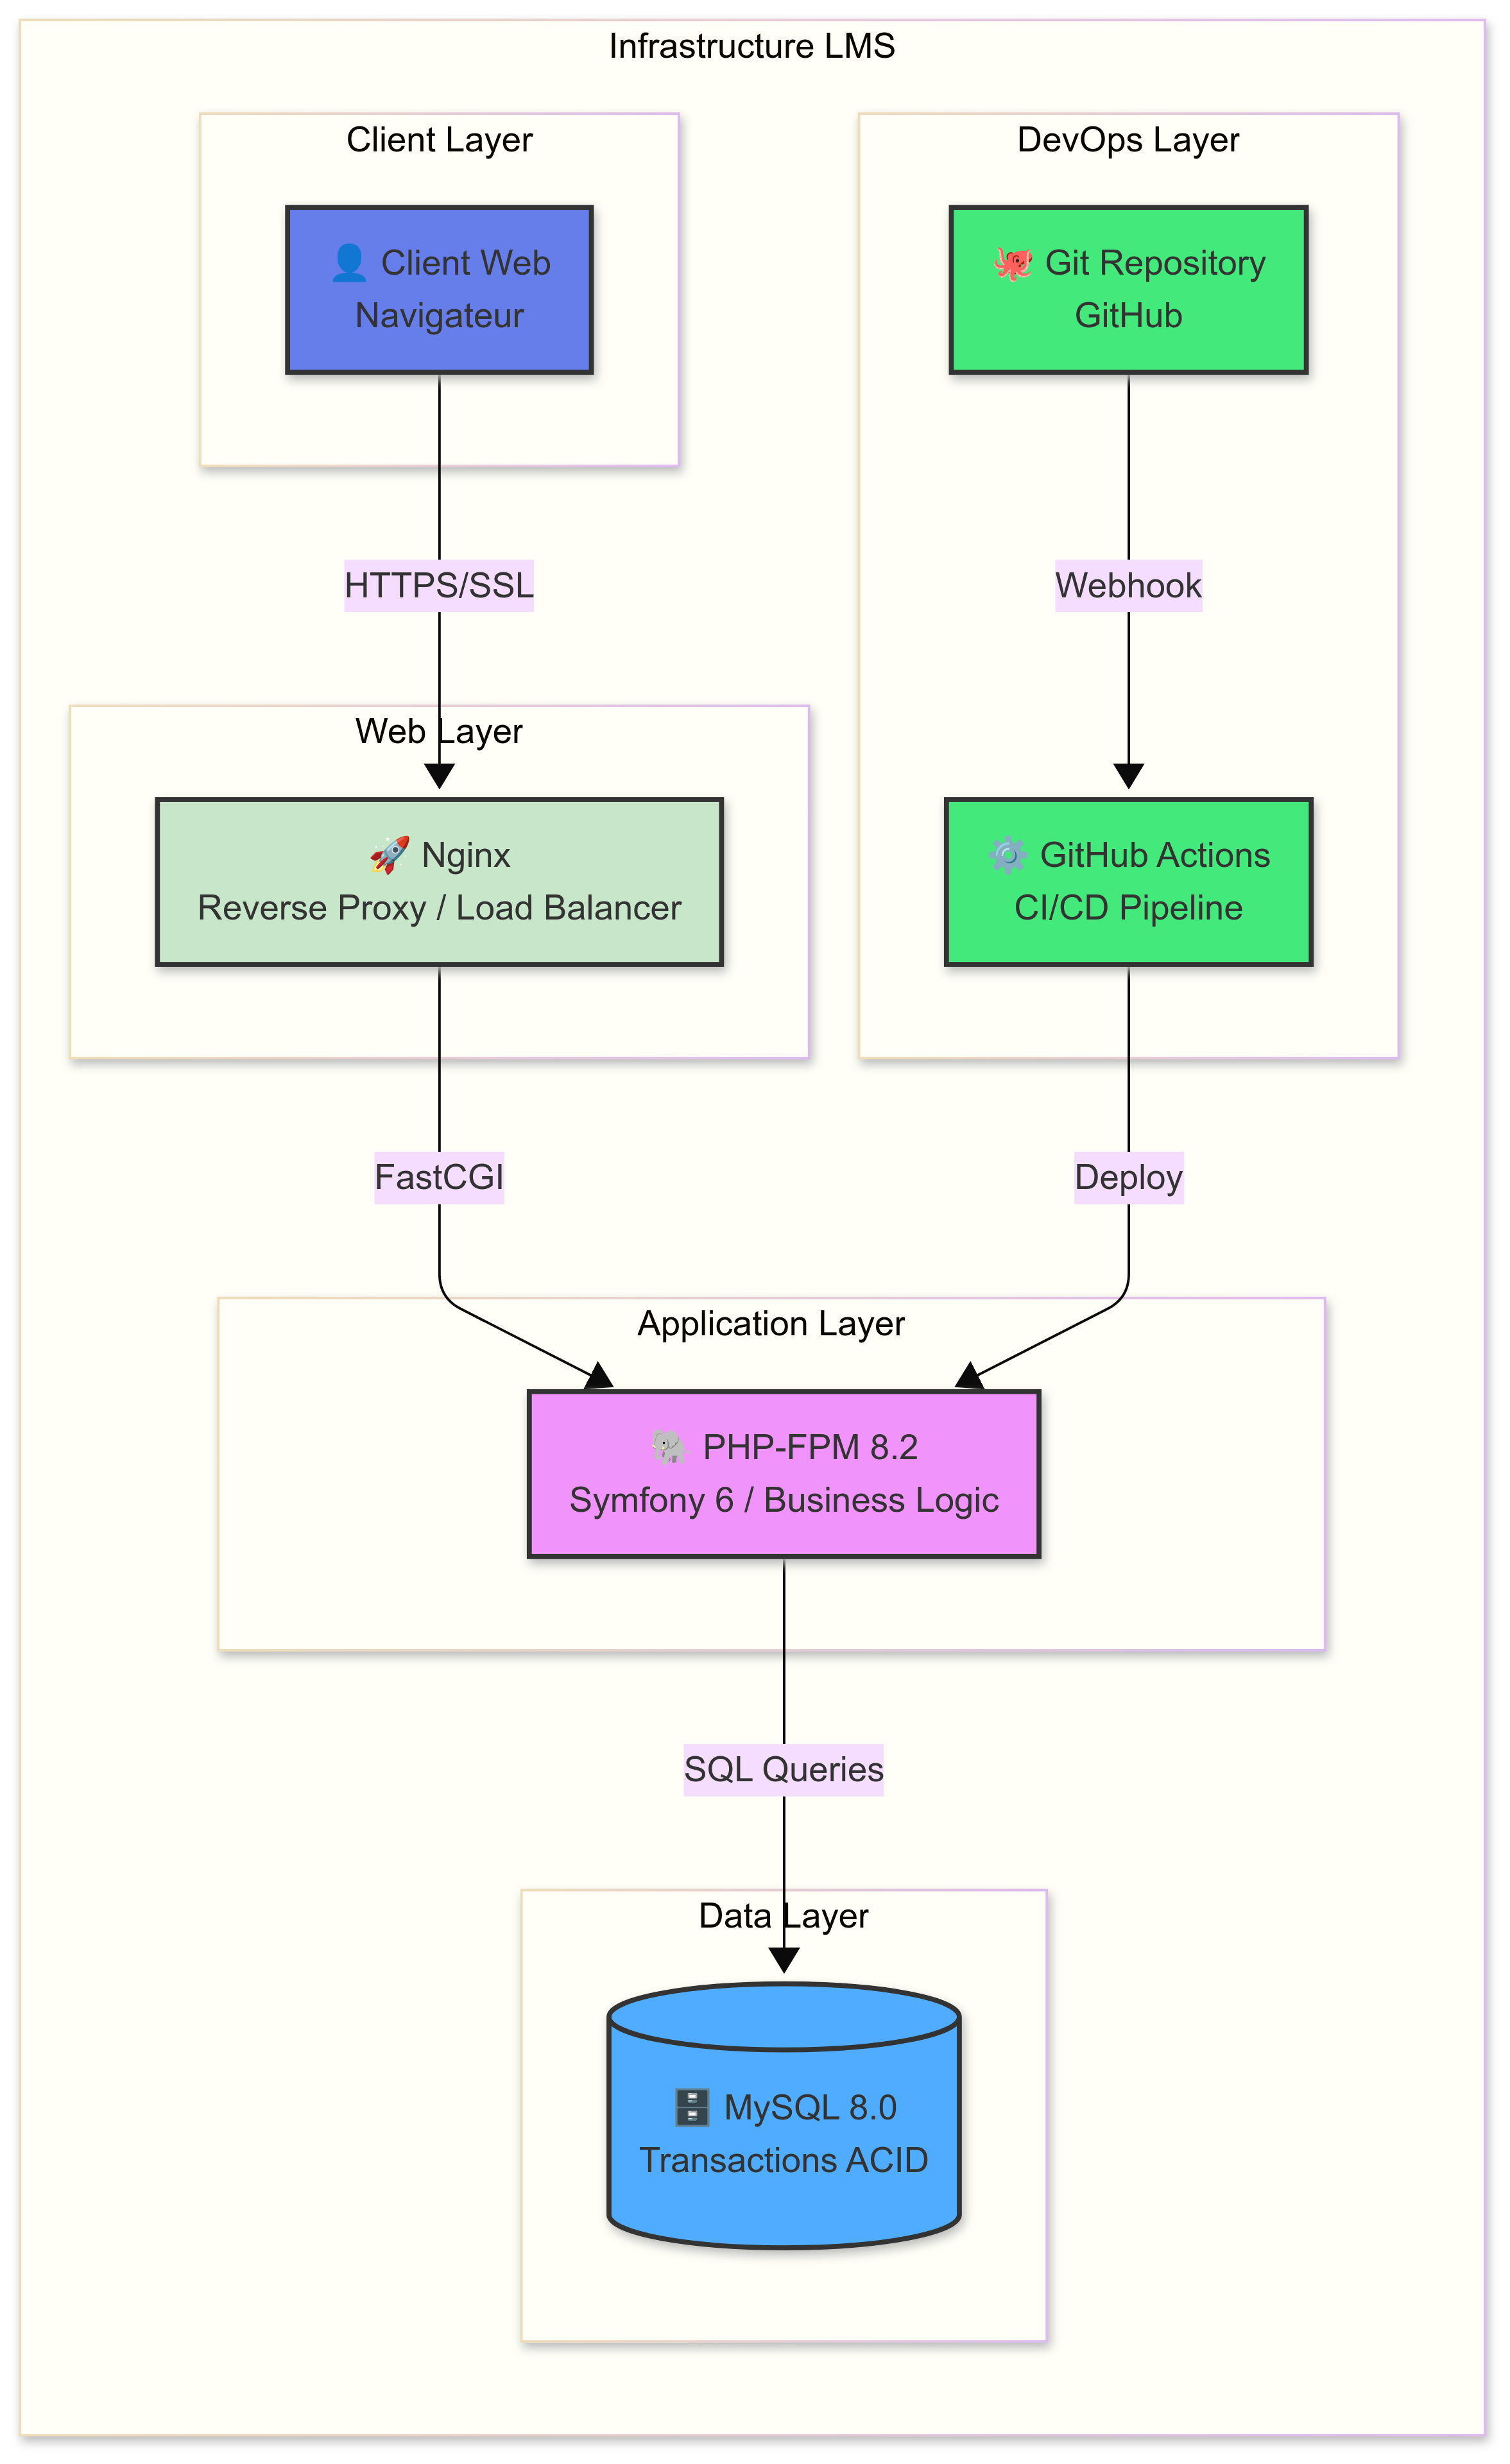
\includegraphics[width=0.8\linewidth]{lmsstructure.png}
\caption{Architecture technique du système Webinar Didier}
\label{fig:archi-tech}
\end{figure}
\newpage

\subsection{Architecture logique}
L'architecture logique décrit comment le code est organisé ainsi que les standards de
programmation suivis au sein de l'environnement TAMTAM.

\subsubsection{Modèle MVC amélioré}
Notre implémentation du pattern MVC intègre des bonnes pratiques spécifiques au contexte LMS :

\begin{figure}[ht!]
\centering
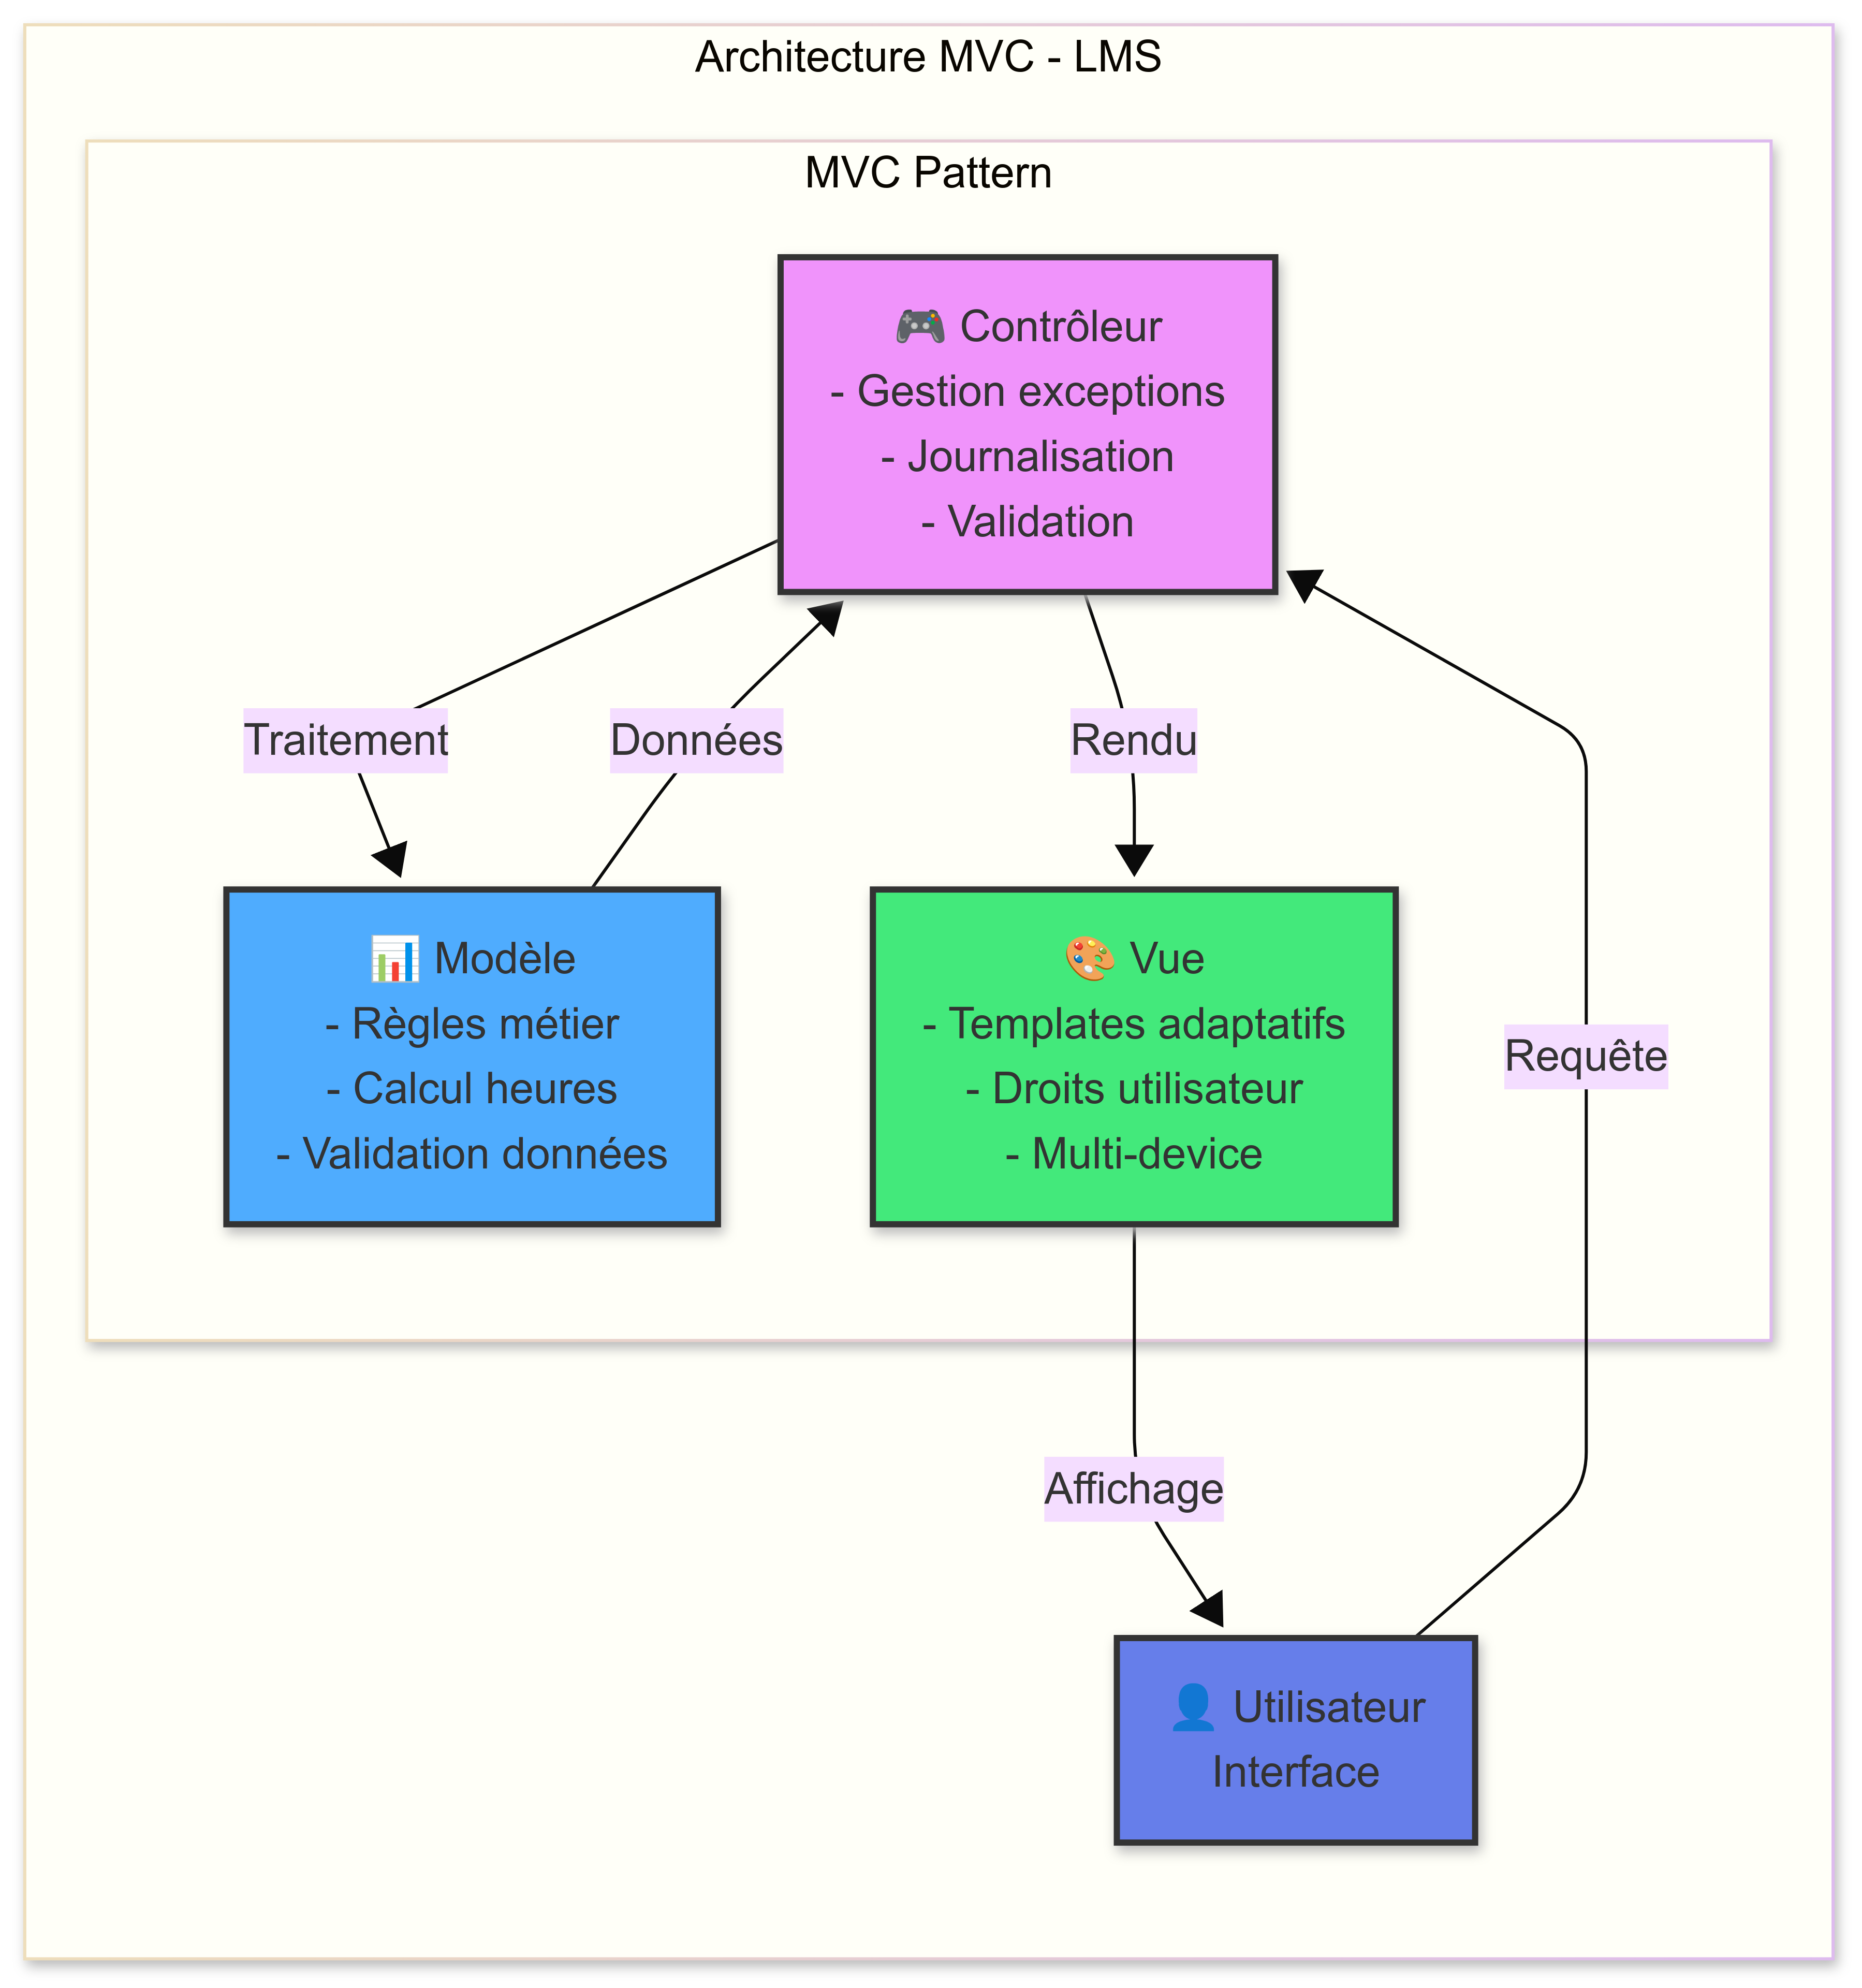
\includegraphics[width=1\linewidth]{mvc.png}
\caption{Flow MVC adapté pour le LMS}
\label{fig:mvc-flow}
\end{figure}

\begin{itemize}
\item \textbf{Modèle} :
\begin{itemize}
\item Couche métier enrichie pour gérer les règles complexes de calcul des heures de formation
\item Validation stricte des données pédagogiques
\end{itemize}
\item \textbf{Vue} :
\begin{itemize}
\item Génération dynamique des interfaces en fonction des droits utilisateur
\item Templates adaptatifs pour différents devices
\end{itemize}
\item \textbf{Contrôleur} :
\begin{itemize}
\item Gestion centralisée des exceptions métier
\item Journalisation détaillée des actions sensibles
\end{itemize}
\end{itemize}

\subsubsection{Structure du projet}
Nous avons conçu l'architecture de notre projet en respectant l'architecture logique établie lors de l'étude technique. Notre application est divisée en deux parties : côté Back-end et côté Front-end. Nous allons présenter les dossiers et les répertoires du projet ainsi que leurs fonctionnalités par rapport à l'objectif du projet LMS.

\paragraph{Architecture logique complète}
La structure du projet LMS s'articule autour d'une architecture modulaire qui sépare clairement les responsabilités entre le back-end et le front-end, tout en maintenant une cohésion fonctionnelle optimale.

\begin{figure}[htbp]
\centering
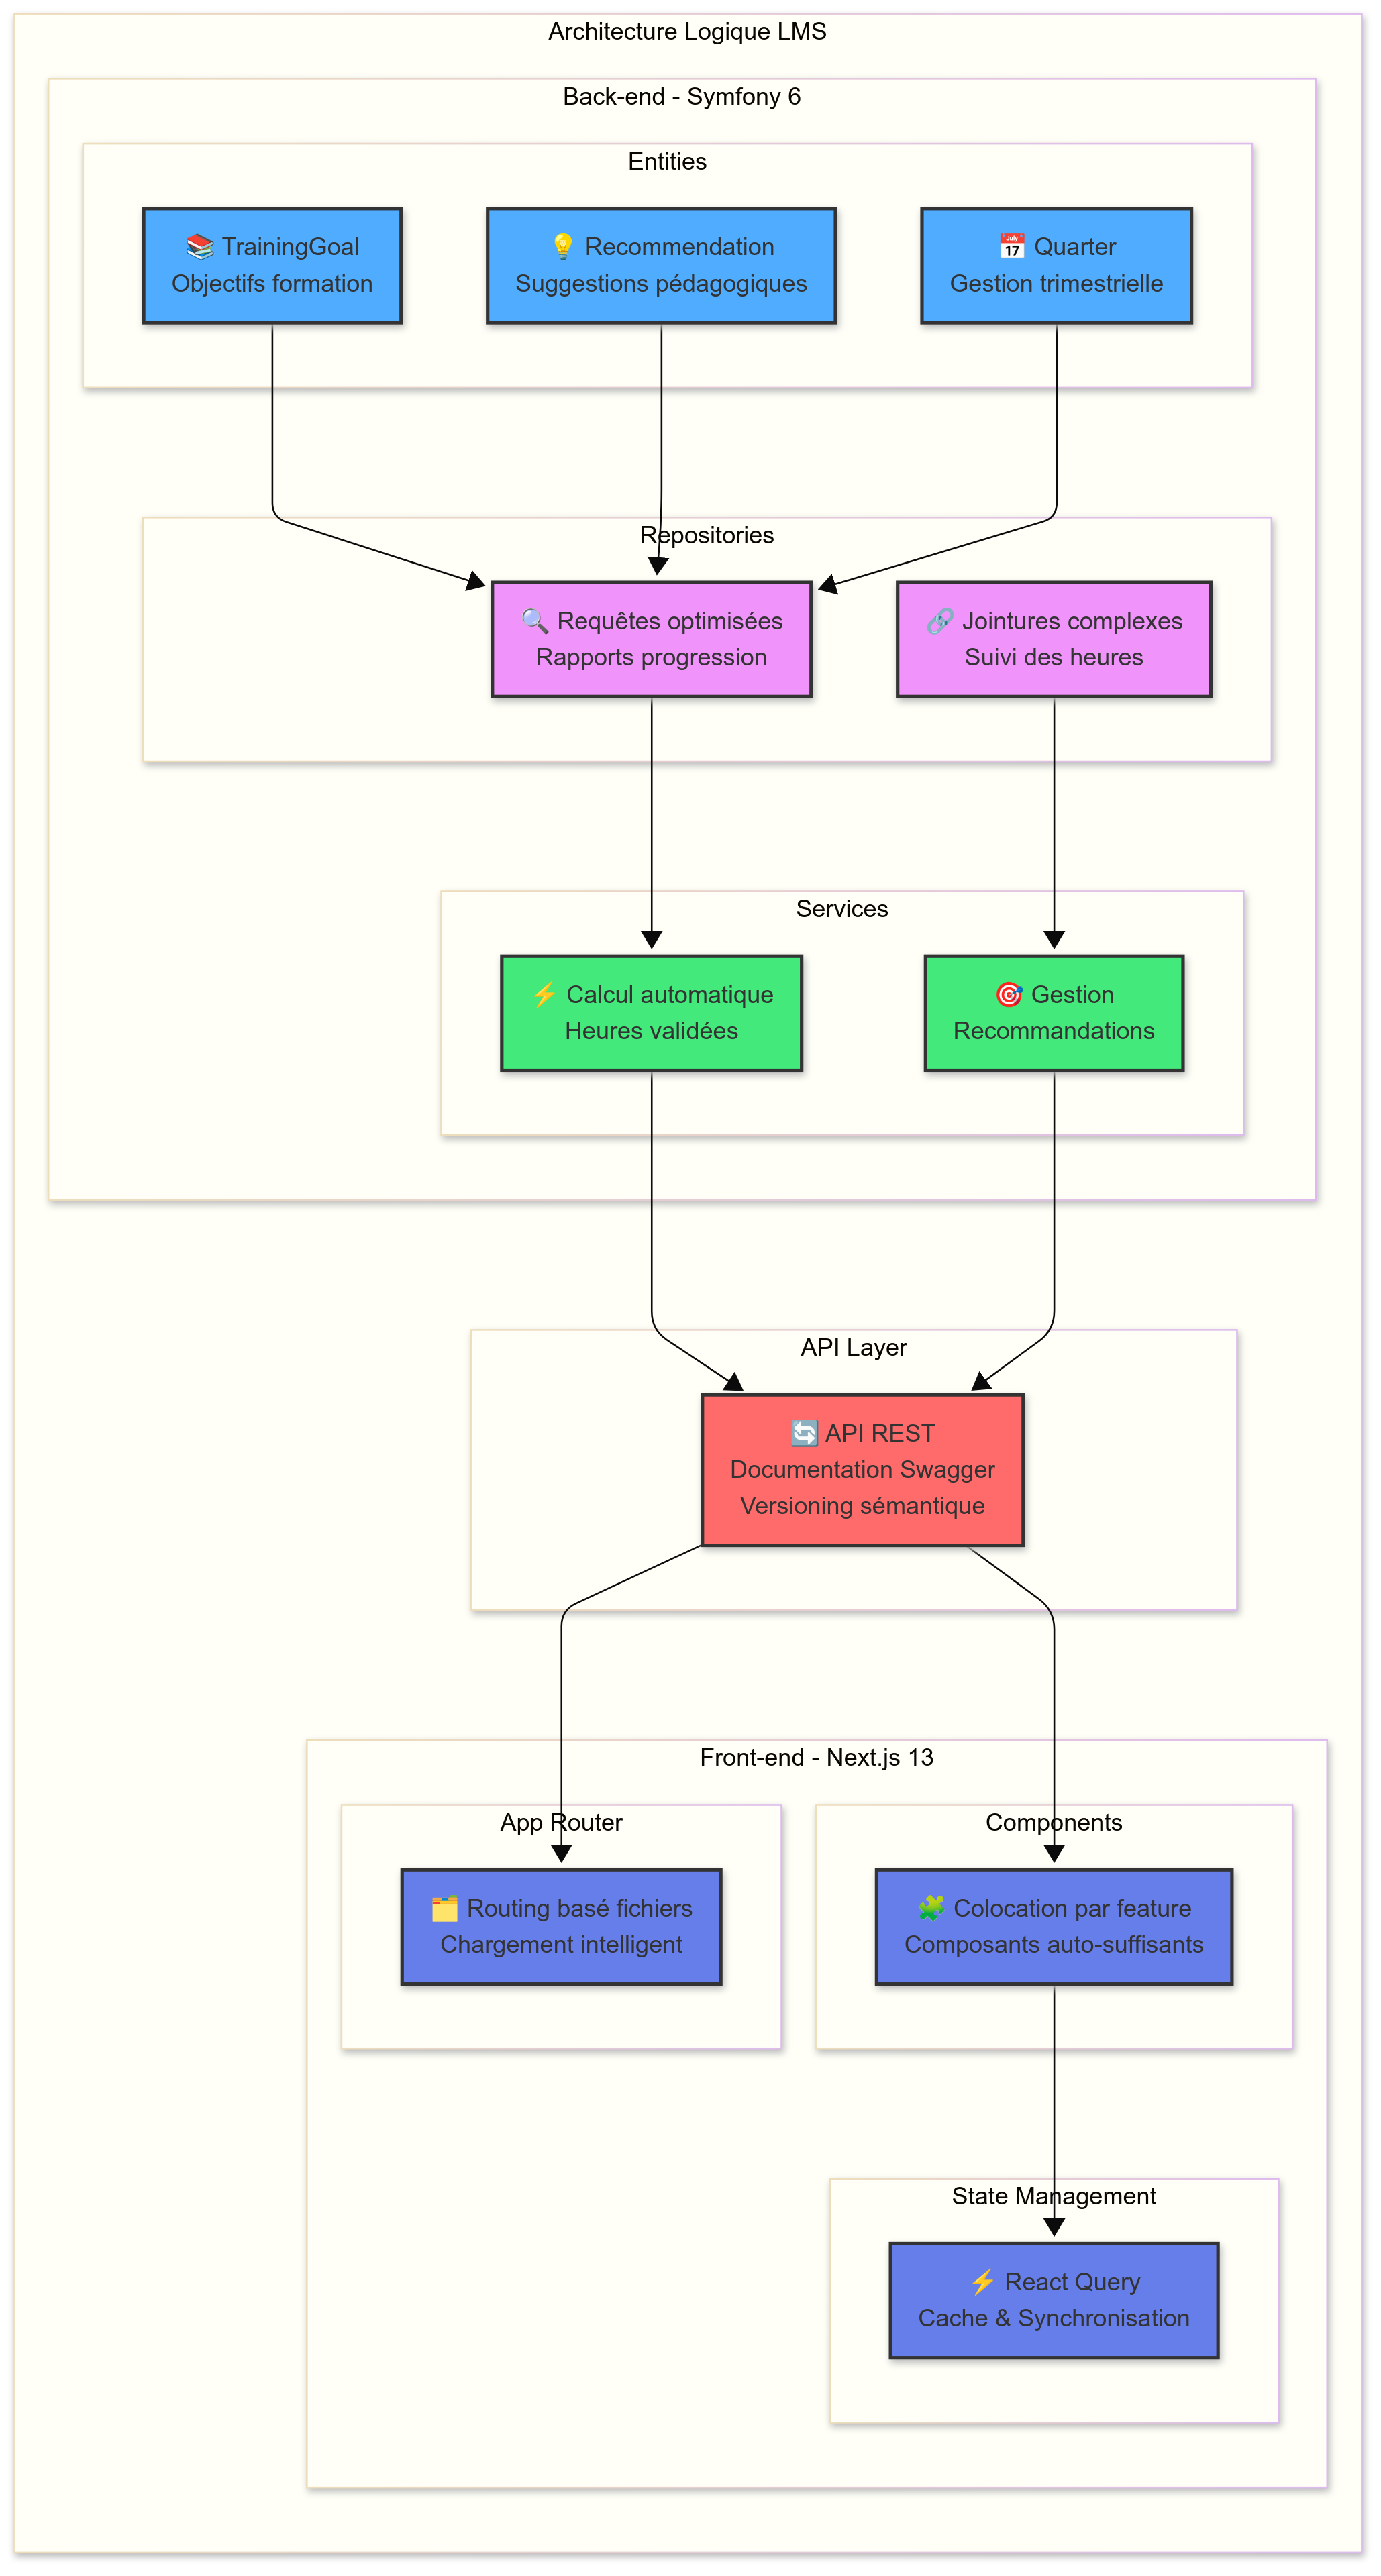
\includegraphics[width=0.8\linewidth]{logique.png}
\caption{Structure logique du projet LMS}
\label{fig:structure-projet}
\end{figure}
\newpage

\paragraph{Côté Back-end}
La partie back-end est centralisée dans une grande API qui contient plusieurs bundles. Chaque projet TAMTAM se représente par un bundle, ce dernier étant un ensemble de fichiers et de répertoires permettant d'implémenter les fonctionnalités d'une application précise. Dans le cas de ce projet, le back-end est représenté par le \texttt{EventBundle} situé sous le dossier \texttt{src/TTP}.

Voici une description de quelques dossiers du Bundle EventBundle :

\begin{itemize}
\item \textbf{Repository} : Contient les requêtes avec jointures complexes, réutilisables pour éviter les duplications de code.
\item \textbf{Resources} : Contient plusieurs fichiers de configuration de l'application en format YAML.
\item \textbf{Controller} : Gère les requêtes HTTP et coordonne les interactions entre les différentes couches de l'application.
\item \textbf{Service} : Un objet PHP remplissant une ou plusieurs fonctions associées à une configuration.
\item \textbf{Entity} : Contient toutes les entités du projet, c'est-à-dire les tables de la base de données.
\item \textbf{Event} : Contient tous les événements déclenchés selon les actions de l'utilisateur.
\item \textbf{Utils} : Classes utilitaires avec des méthodes prédéfinies réutilisables.
\item \textbf{Tests} : Tests fonctionnels et unitaires, ainsi qu'un dossier DataFixtures pour les données de test.
\item \textbf{Validator} : Validation des attributs des entités, par filtrage ou par rôle.
\end{itemize}

Entités principales dans le système LMS :
\begin{itemize}
\item \texttt{TrainingGoal} — Objectifs de formation
\item \texttt{Recommendation} — Suggestions pédagogiques
\item \texttt{Quarter} — Périodes trimestrielles
\end{itemize}

\paragraph{Côté Front-end}
Notre projet Next.js 13.4 adopte l'approche de colocation pour s'aligner avec la nouvelle architecture Next.js. Nous utilisons la convention \texttt{kebab-case} pour nommer les fichiers et dossiers, et travaillons avec TypeScript.

La structure de dossiers du projet est la suivante :
\begin{itemize}
\item \textbf{src/} : dossier racine de l'application.
\item \textbf{src/app/[lang]/feature/} : code d'une fonctionnalité (page, composants, hooks, services, constantes, types).
\item \textbf{src/app/[lang]/feature/page.tsx} : point d'entrée de la page.
\item \textbf{src/app/[lang]/feature/components/} : composants propres à la fonctionnalité.
\item \textbf{src/common/} : éléments partagés (components, services, constants, types, styles).
\item \textbf{src/common/services/misc/fetch-api-wrapper.ts} : wrapper d'appels API communs.
\item \textbf{src/common/constants/routes.ts} : définition centralisée des routes.
\item \textbf{src/contexts/} : providers de contexte.
\item \textbf{src/i18n/} : internationalisation et localisation.
\item \textbf{src/middleware.ts} : logique middleware (authentification, autorisation, redirections).
\end{itemize}

%------------------------------------------------------------
\section{Qualité de code}

\subsection{Outils de linting}
Nous appliquons une discipline stricte de qualité de code avec :
\begin{itemize}
\item \textbf{ESLint} : Configuration personnalisée basée sur Airbnb, détection des patterns problématiques, règles TypeScript strictes.
\item \textbf{Prettier} : Formatage automatique du code avec configuration partagée en équipe.
\item \textbf{Stylelint} : Cohérence CSS/SCSS et bonnes pratiques de style.
\end{itemize}

\subsection{Git Hooks}
Automatisation des vérifications via Husky :
\begin{itemize}
\item \textbf{pre-commit} : Exécution de lint-staged et vérification des types TypeScript.
\item \textbf{commit-msg} : Validation du format Conventional Commits. Exemple : \texttt{feat(lms): ajout calcul heures trimestrielles}.
\item \textbf{pre-push} : Exécution des tests unitaires et vérification de la build.
\end{itemize}

\subsection{Conventional Commits}
Standardisation des messages de commit :

\begin{longtable}{|l|p{10cm}|}
\hline
\textbf{Type} & \textbf{Usage} \\ \hline
\texttt{feat} & Nouvelle fonctionnalité \\ \hline
\texttt{fix} & Correction de bug \\ \hline
\texttt{docs} & Modification de documentation \\ \hline
\texttt{style} & Changement de formatage \\ \hline
\texttt{refactor} & Modification de code sans impact fonctionnel \\ \hline
\texttt{perf} & Amélioration de performance \\ \hline
\texttt{test} & Ajout ou modification de tests \\ \hline
\texttt{chore} & Tâches de maintenance \\ \hline
\end{longtable}

%------------------------------------------------------------
\section{Spécification technologique}
Pour décrire les spécifications technologiques de notre application, nous allons présenter les
technologies utilisées dans le développement.

\subsection{Outils de développement}

% ==============================================================
% MACRO : logo à gauche + titre + texte à droite (style image)
% ==============================================================
\newcommand{\techitem}[4][l]{%
\noindent
\begin{minipage}[t]{0.18\textwidth}
    \raggedright
    \vspace{0pt}
    \includegraphics[width=0.90\linewidth]{#2}\\[4pt]
    {\small\textit{Figure : logo #3}}
\end{minipage}%
\hspace{0.04\textwidth}%
\begin{minipage}[t]{0.75\textwidth}
    \vspace{0pt}
    {\large $\clubsuit$ \quad \textbf{#3 :}}\\[6pt]
    #4
\end{minipage}
\vspace{1.2em}
}

% ---- Node.js ----
\techitem{Chapters/img/nodejs.png}{Node.JS}{%
Node.js est \underline{une plateforme de développement JavaScript intégrant un serveur HTTP}.
Son fonctionnement se base sur une boucle événementielle qui lui permet le support de fortes montées en charge.
Dans notre projet, Node.js est utilisé pour bâtir des APIs légères, des services en temps réel
et des outils d'automatisation (scripts, watchers, serveurs de développement).%
}

% ---- React.js ----
\techitem{Chapters/img/react.png}{React.js}{%
React.js est une bibliothèque JavaScript dédiée à la construction d'interfaces utilisateur réactives et modulaires.
Son modèle basé sur les composants favorise la réutilisabilité et la maintenabilité du code front-end.
Dans notre contexte Webinar, il facilite la conception d'écrans interactifs et la gestion d'états complexes
via le Virtual DOM.%
}

% ---- Meteor.js ----
\techitem{Chapters/img/metor.png}{Meteor.js}{%
Meteor.js est une plateforme JavaScript full-stack qui simplifie le développement d'applications en temps réel.
Elle fournit un environnement unifié client/serveur et utilise le protocole DDP pour la synchronisation des données.
Dans le cadre du LMS, Meteor est utilisé pour les fonctionnalités collaboratives en temps réel
(chat, notifications, synchronisation d'état).%
}

% ---- Symfony ----
\techitem{logos/symfony.png}{Symfony Framework}{%
Symfony est un framework PHP de développement d'applications web fournissant une architecture MVC robuste
et des composants réutilisables. Il offre un routing flexible, un conteneur d'injection de dépendances,
un système de templating Twig, et de nombreux bundles. Sa philosophie DRY (\textit{Don't Repeat Yourself})
favorise la réutilisabilité du code et réduit les erreurs de développement.%
}

% ---- Doctrine ----
\techitem{logos/doctrine.png}{Doctrine}{%
Doctrine est un ORM (Object-Relational Mapping) pour PHP permettant de manipuler les entités de la base de données.
Il est livré par défaut avec Symfony et crée l'illusion d'une base de données orientée objet à partir d'une
base de données relationnelle en définissant des correspondances entre les deux mondes.%
}

% ---- PHPUnit ----
\techitem{logos/phpunit.png}{PHPUnit}{%
PHPUnit est un framework open source de tests unitaires dédié au langage PHP.
Il permet l'implémentation de tests de régression en vérifiant que les exécutions correspondent aux
assertions prédéfinies. Les appels aux services, bases de données ou fichiers sont simulés (\textit{mocked})
afin d'assurer des tests vraiment unitaires.%
}

% ---- Swagger ----
\techitem{logos/swagger.png}{Swagger / OpenAPI}{%
Swagger est un ensemble d'outils open source permettant de concevoir, documenter et consommer des services web REST.
Il utilise la spécification OpenAPI pour décrire les APIs de manière standardisée et génère une documentation
interactive permettant de tester les endpoints directement depuis l'interface web.%
}

% ---- Next.js ----
\techitem{logos/next.png}{Next.js}{%
Next.js est un framework React de nouvelle génération permettant de créer des applications web modernes
avec un rendu côté serveur (SSR) et une génération de sites statiques (SSG) optimisée.
Son App Router introduit les Server Components, le routage automatique basé sur les fichiers,
et le support natif de TypeScript.%
}

% ---- TypeScript ----
\techitem{logos/Typescript_logo_2020.png}{TypeScript}{%
TypeScript est un sur-ensemble typé de JavaScript qui compile vers du JavaScript standard.
Il apporte un système de types statiques permettant de détecter les erreurs à la compilation
plutôt qu'à l'exécution. Dans notre projet, TypeScript est utilisé côté front-end pour améliorer
la maintenabilité, la lisibilité et la robustesse du code.%
}

%------------------------------------------------------------
\subsection{GitHub Actions}
Pipeline automatisé avec :
\begin{itemize}
\item \textbf{Tests unitaires} : Exécution sur chaque push
\item \textbf{Analyse de code} : Vérification des vulnérabilités
\item \textbf{Déploiement} : Mise en production conditionnelle
\end{itemize}

Le processus d'intégration continue du LMS Didier garantit la qualité et la fiabilité de chaque déploiement
grâce à un pipeline automatisé sophistiqué.

\begin{figure}[htbp]
\centering
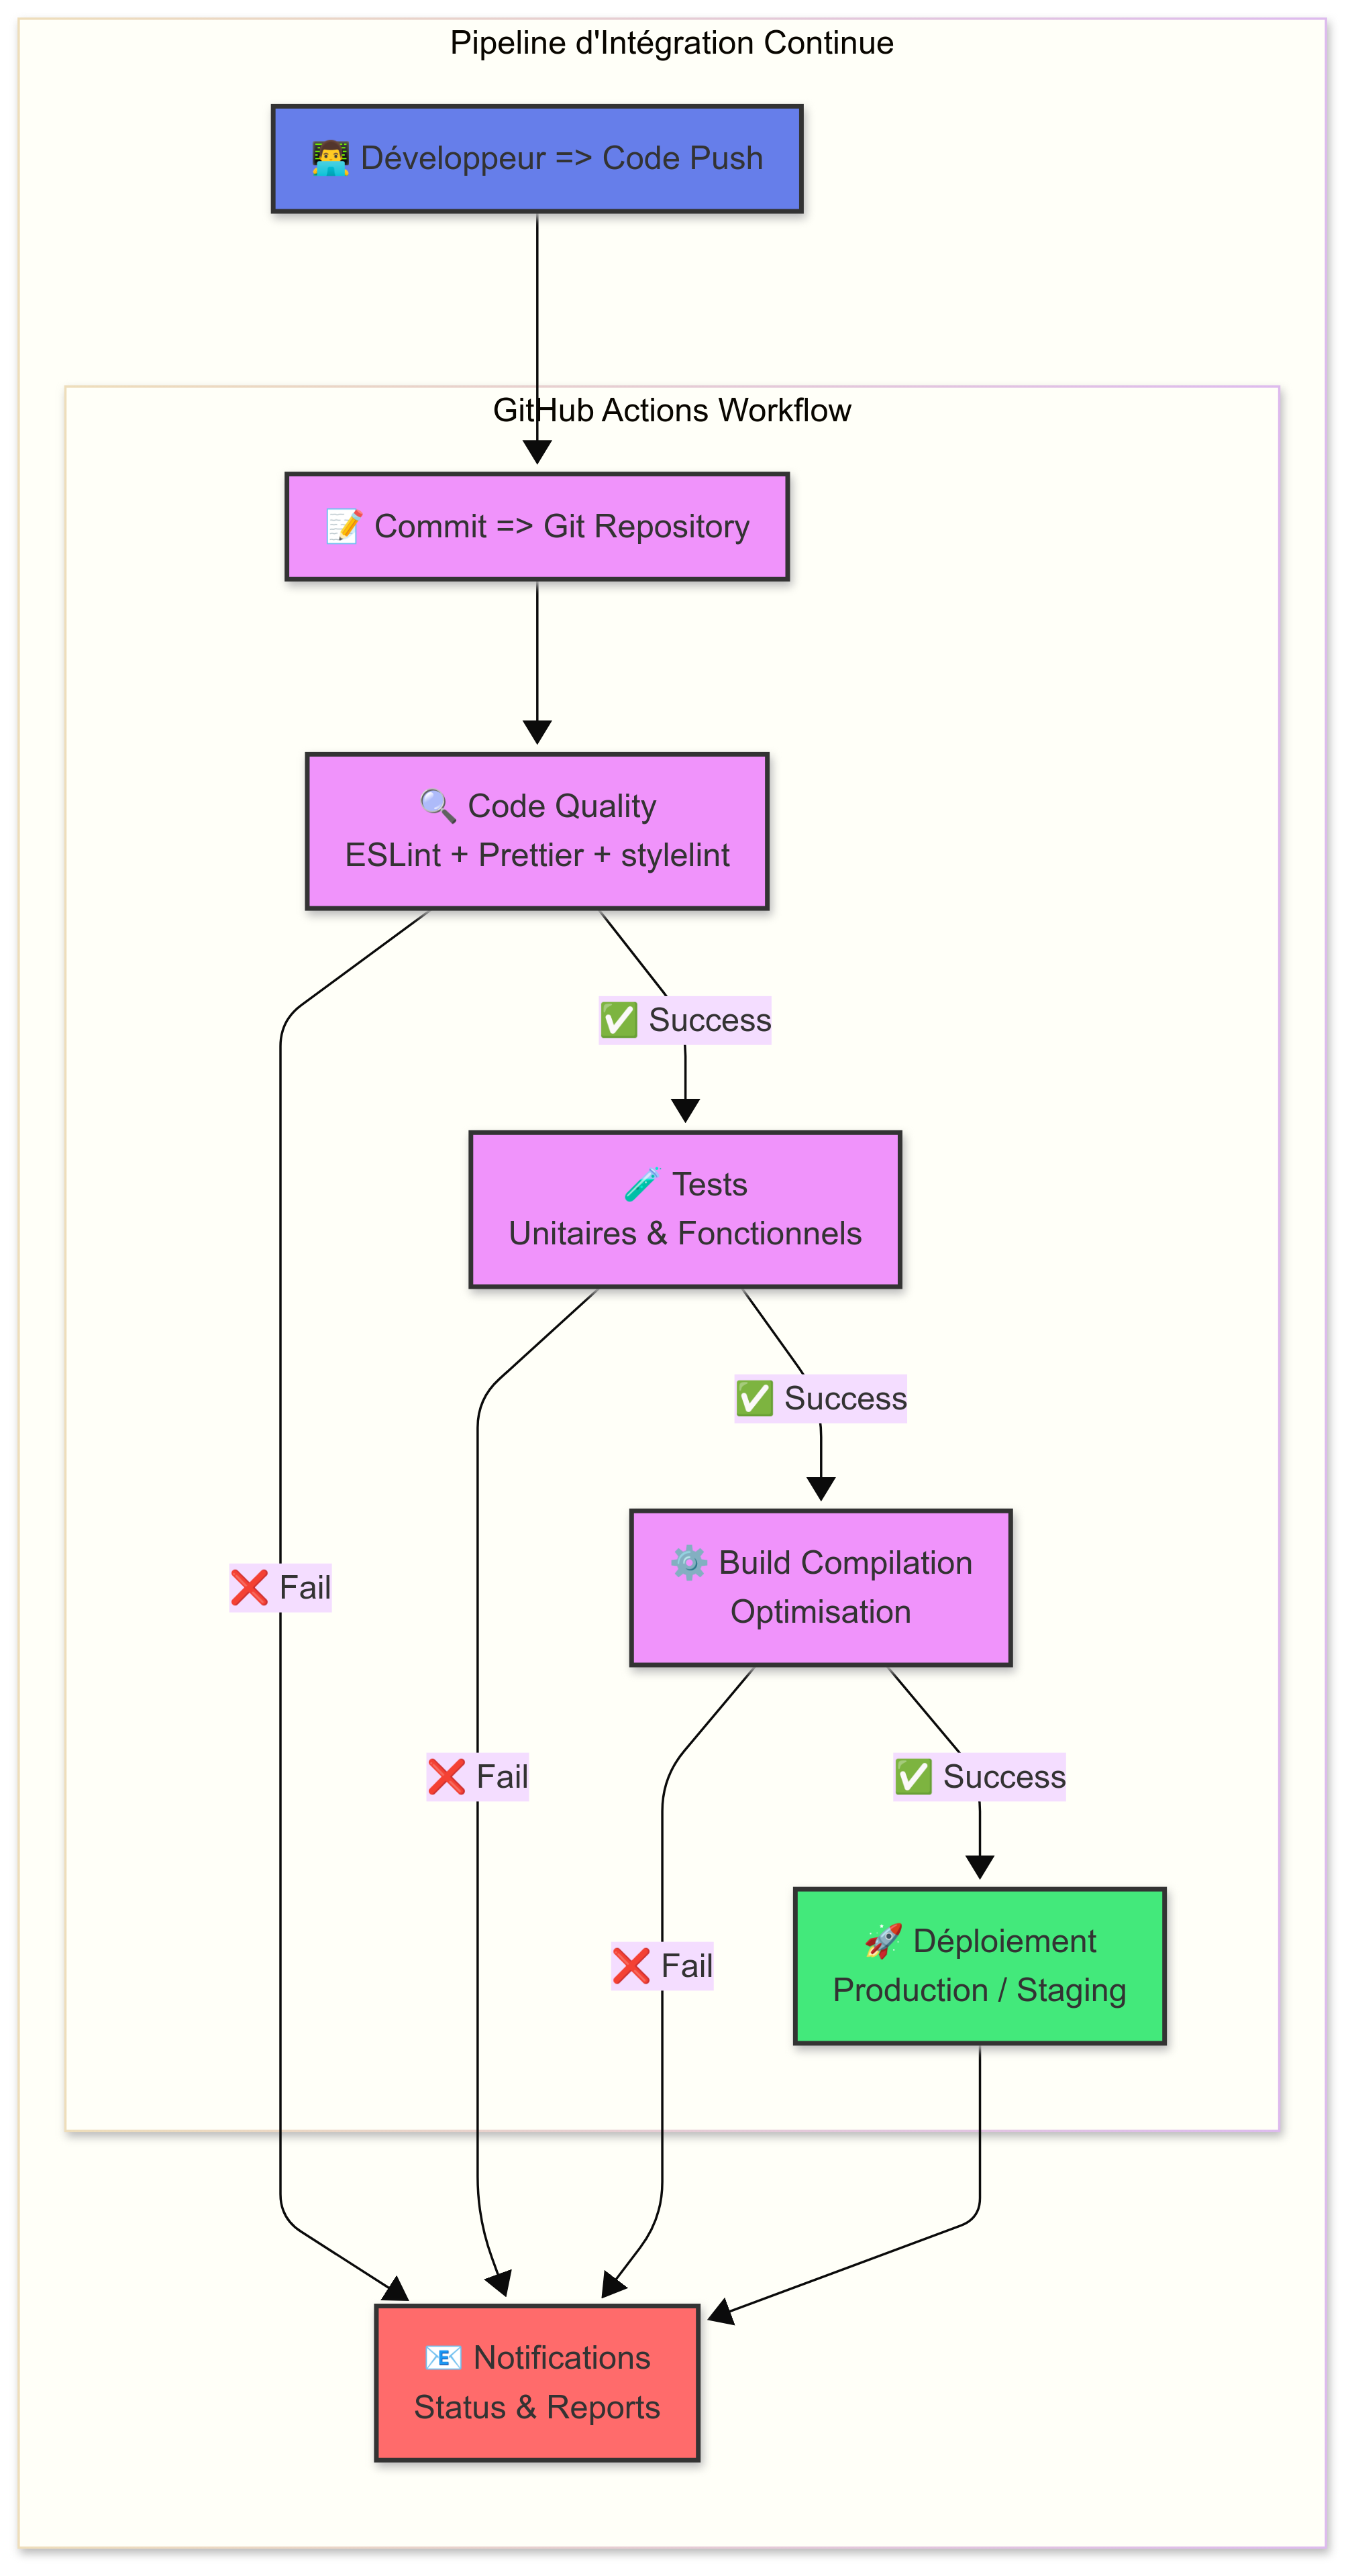
\includegraphics[width=0.8\linewidth]{pipeline.png}
\caption{Pipeline GitHub Actions automatisé}
\label{fig:cicd-pipeline}
\end{figure}

\subsection{Release automation}
Gestion sémantique des versions avec \texttt{release-it} :
\begin{itemize}
\item \textbf{Changelog} : Génération automatique
\item \textbf{Versioning} : Respect de SemVer
\item \textbf{GitHub Releases} : Publication automatisée
\end{itemize}

%------------------------------------------------------------
\section{Architecture de déploiement}

\subsection{Infrastructure de production}

L'architecture de déploiement du LMS Didier privilégie la haute disponibilité et la performance
pour répondre aux exigences critiques des fiduciaires belges. Notre infrastructure est conçue pour
supporter une montée en charge progressive tout en maintenant une qualité de service optimale.

\begin{figure}[htbp]
\centering
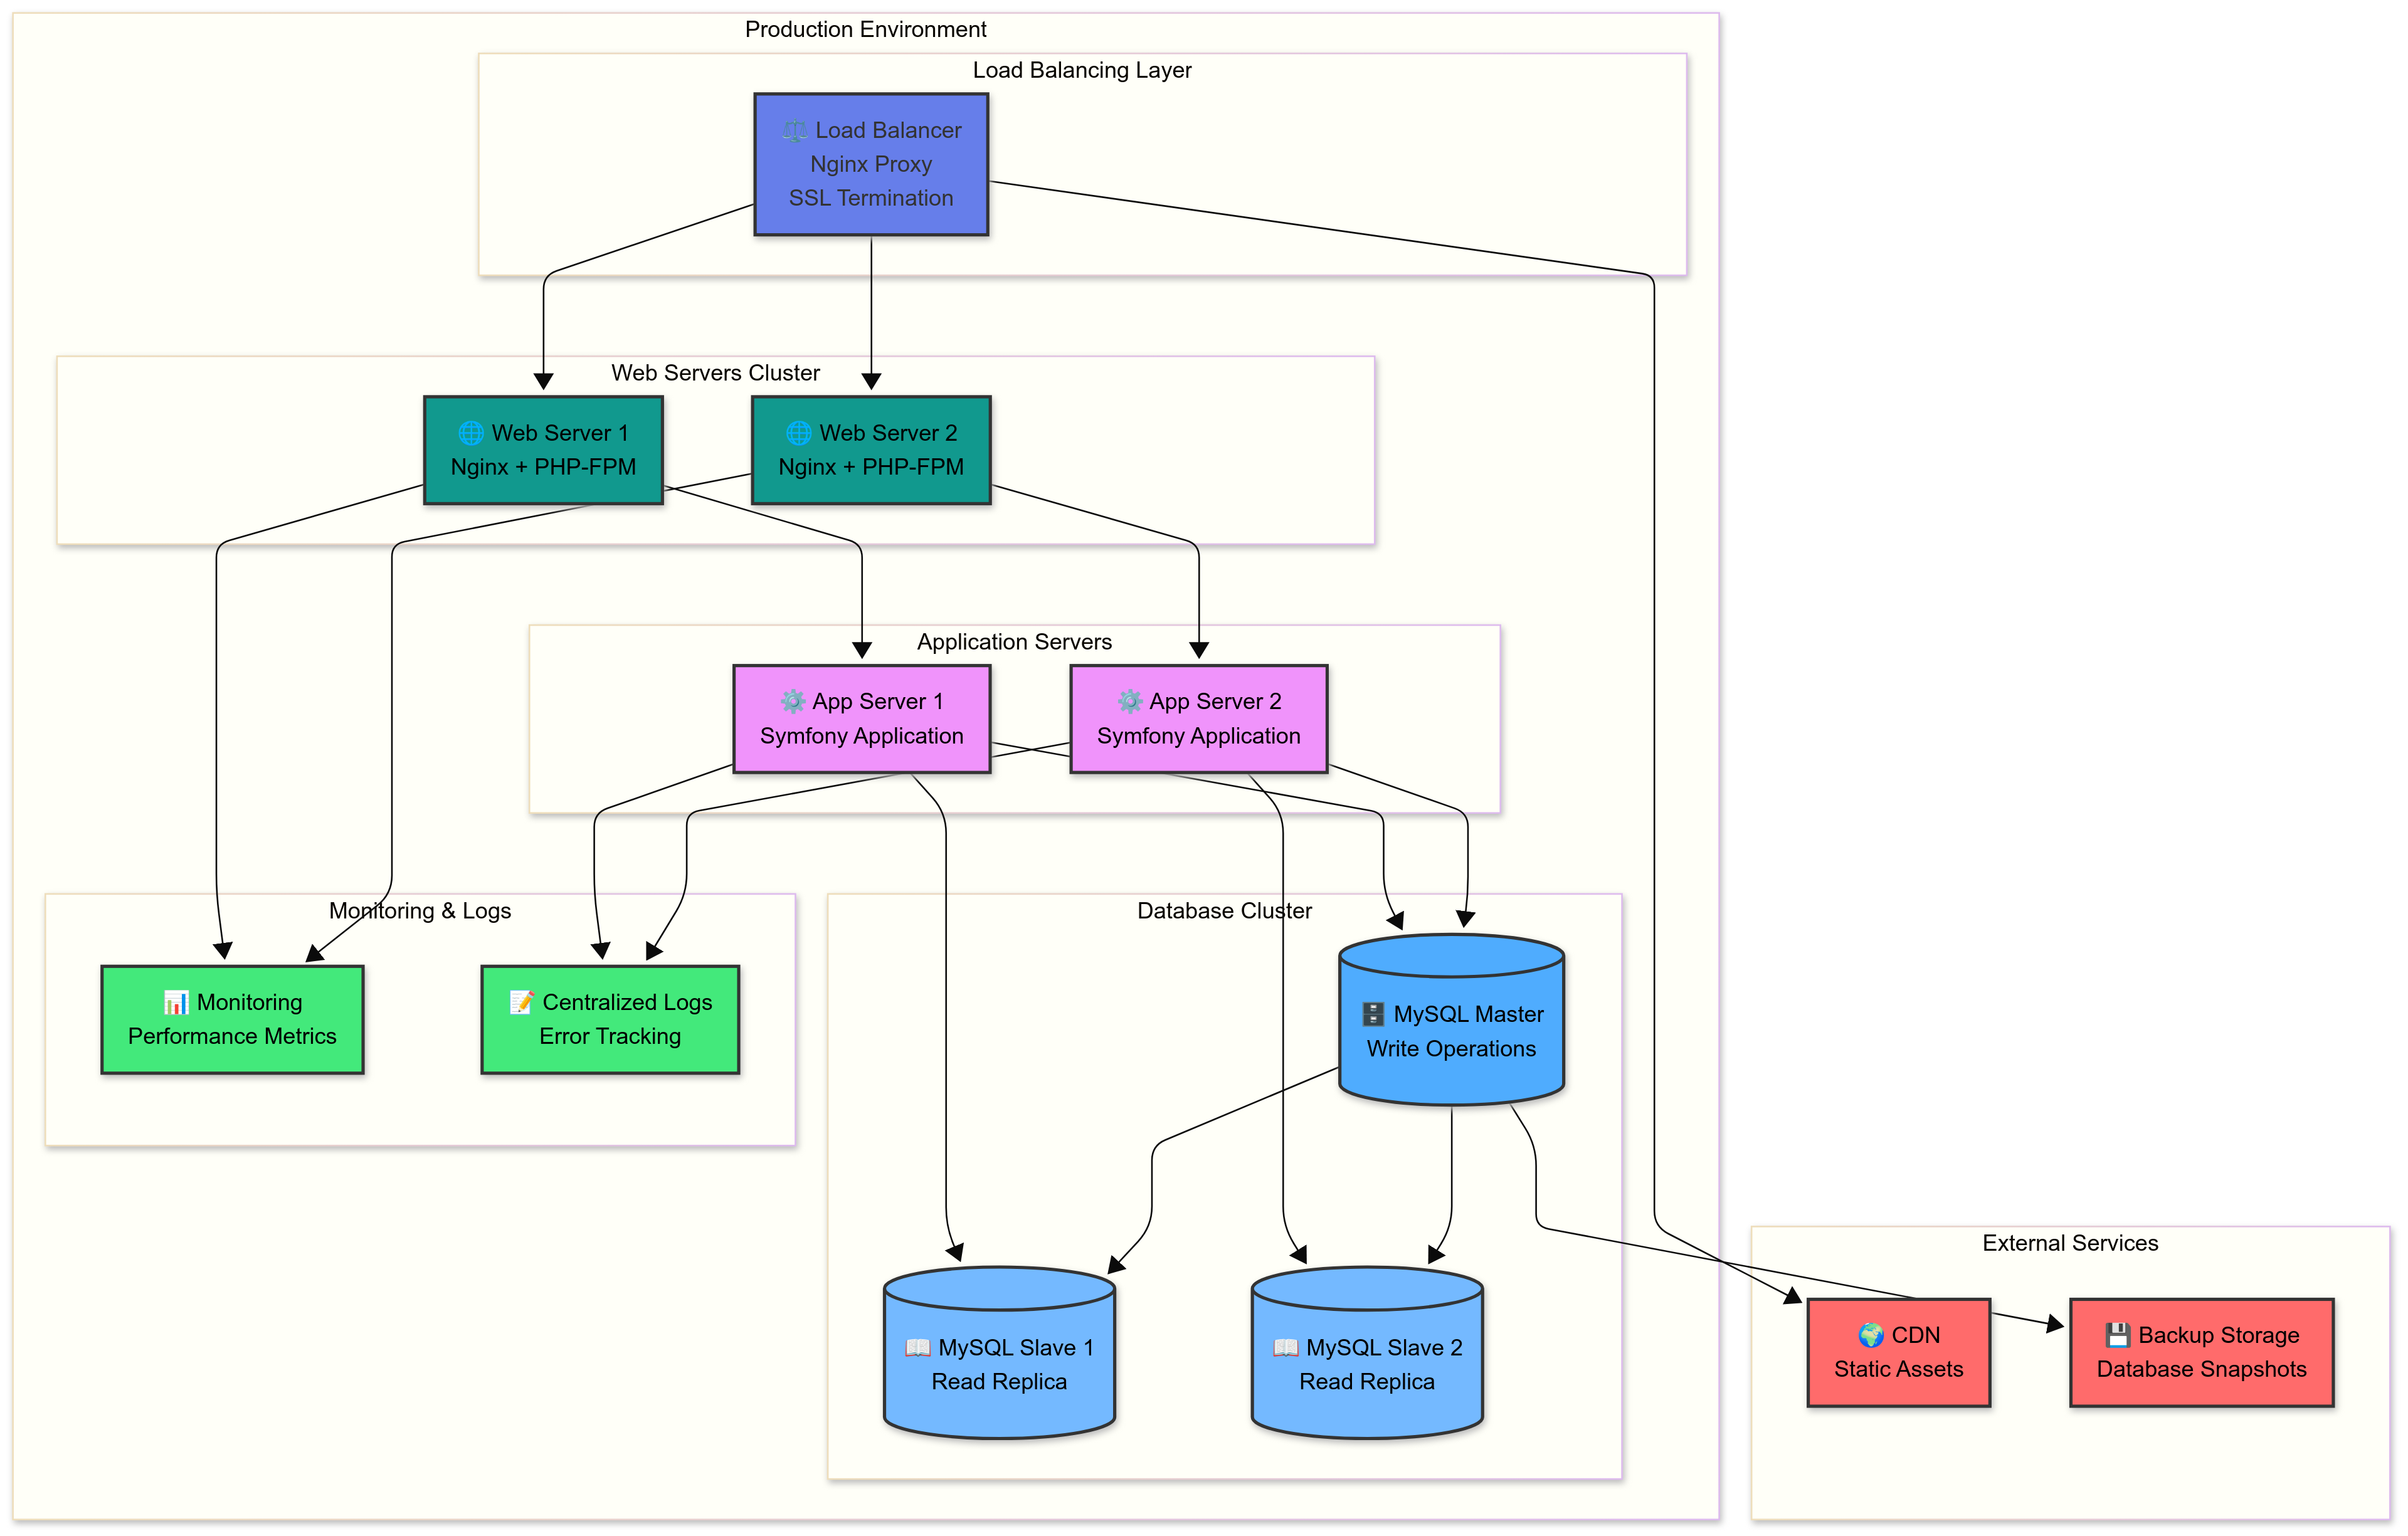
\includegraphics[width=1.0\linewidth]{Chapters/production.png}
\caption{Architecture de déploiement haute disponibilité}
\label{fig:deployment-arch}
\end{figure}

\subsection{Caractéristiques de l'infrastructure}
\begin{itemize}
\item \textbf{Haute disponibilité} : Redondance à tous les niveaux pour éliminer les points de défaillance unique
\item \textbf{Scalabilité horizontale} : Ajout transparent de serveurs selon la charge
\item \textbf{Répartition de charge} : Distribution intelligente du trafic via Nginx
\item \textbf{Base de données distribuée} : Configuration Master/Slave pour optimiser les performances lecture/écriture
\item \textbf{Monitoring continu} : Surveillance proactive des métriques de performance
\item \textbf{Sauvegarde automatisée} : Protection des données critiques avec snapshots réguliers
\end{itemize}

%------------------------------------------------------------
\section{Conclusion}
L'architecture technique du projet TT Webinar combine performance et maintenabilité grâce à des choix
technologiques éprouvés et une infrastructure moderne. Les diagrammes présentés illustrent la robustesse
de notre approche, depuis l'architecture physique jusqu'au déploiement en production. Les outils de qualité
et d'intégration continue garantissent la pérennité du code, tandis que l'architecture de déploiement assure
une disponibilité optimale pour les utilisateurs finaux. Le chapitre suivant détaillera les aspects spécifiques
d'implémentation du projet TT Webinar.
\chapter{Réalisation}

\section{Introduction}
L'objectif de cette partie est de donner aux lecteurs de ce rapport un aperçu détaillé des différentes interfaces du système de gestion de l'apprentissage (LMS) de United Associates, développé en partenariat avec DEG\&PARTNERS. Ce chapitre présente les fonctionnalités offertes aux différents acteurs du système, notamment les collaborateurs, les gestionnaires et les formateurs.

\section{Présentation des interfaces}

\subsection{Interface principale du tableau de bord}
L'interface principale du LMS constitue le point d'entrée central pour tous les utilisateurs. Elle présente une vue d'ensemble personnalisée des activités de formation et des objectifs temporels.

\begin{figure}[H]
    \centering
    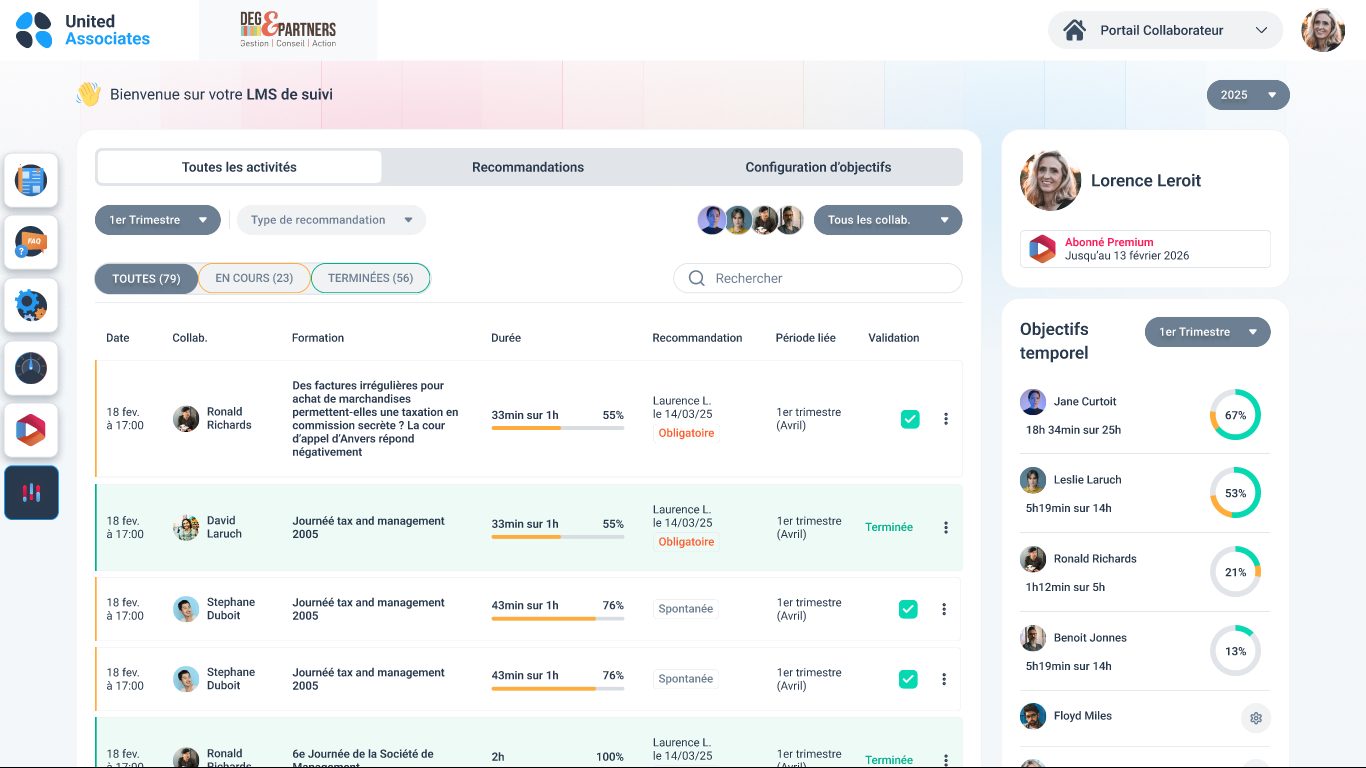
\includegraphics[width=\textwidth]{realisation/toutactivite.png}
    \caption{Interface principale du LMS}
    \label{fig:interface_principale}
\end{figure}

Cette interface comprend plusieurs sections principales :
\begin{itemize}
    \item \textbf{Barre de navigation} : Permettant l'accès aux différentes fonctionnalités (Toutes les activités, Recommandations, Configuration d'objectifs)
    \item \textbf{Panneau d'activités} : Affichant les formations en cours, terminées et à venir avec leurs statuts respectifs
    \item \textbf{Section objectifs temporels} : Présentant les progrès individuels des collaborateurs avec des indicateurs visuels
\end{itemize}

\subsection{Interface de gestion des recommandations}
Cette interface permet aux utilisateurs de consulter et gérer les recommandations de formation personnalisées.

\begin{figure}[H]
    \centering
    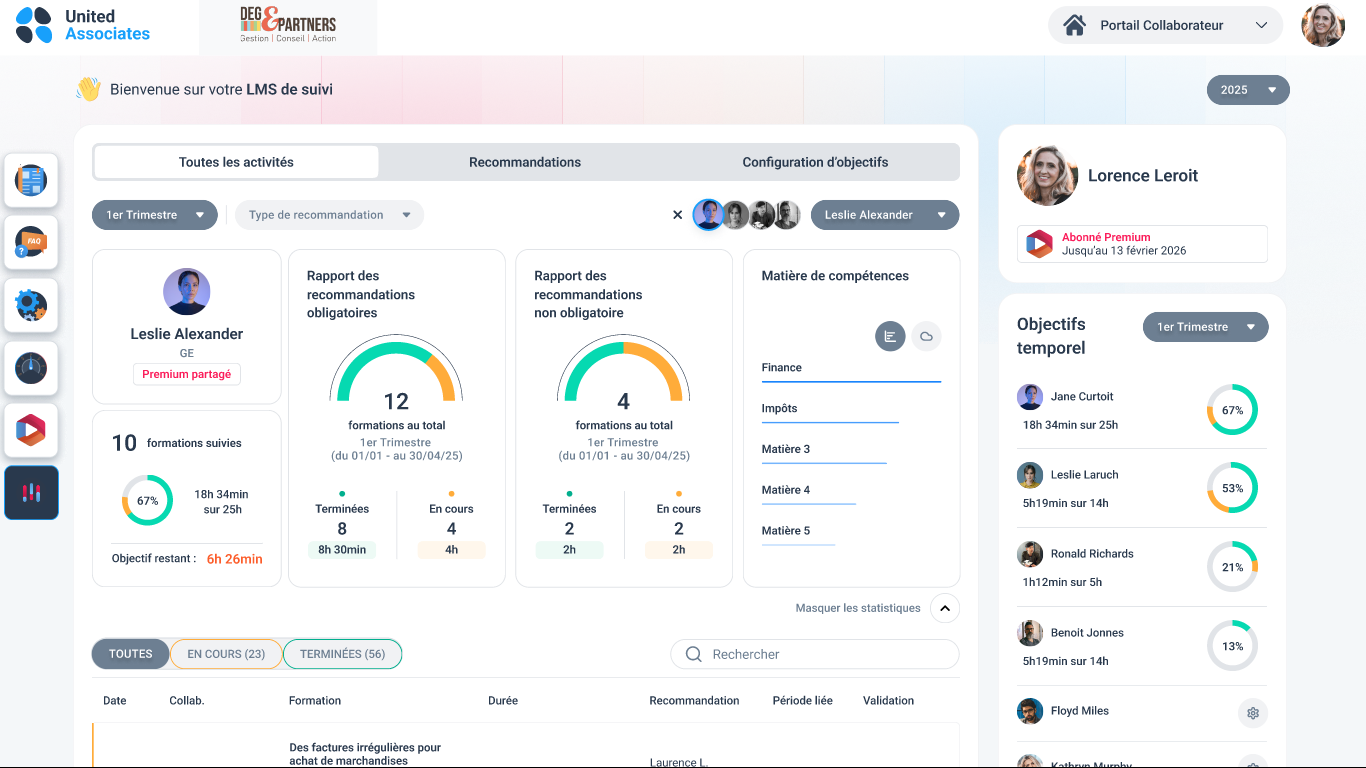
\includegraphics[width=\textwidth]{realisation/user.png}    
    \caption{Interface des recommandations d'un collaborateur}
    \label{fig:interface_recommandations}

\end{figure}
\begin{figure}[H]
    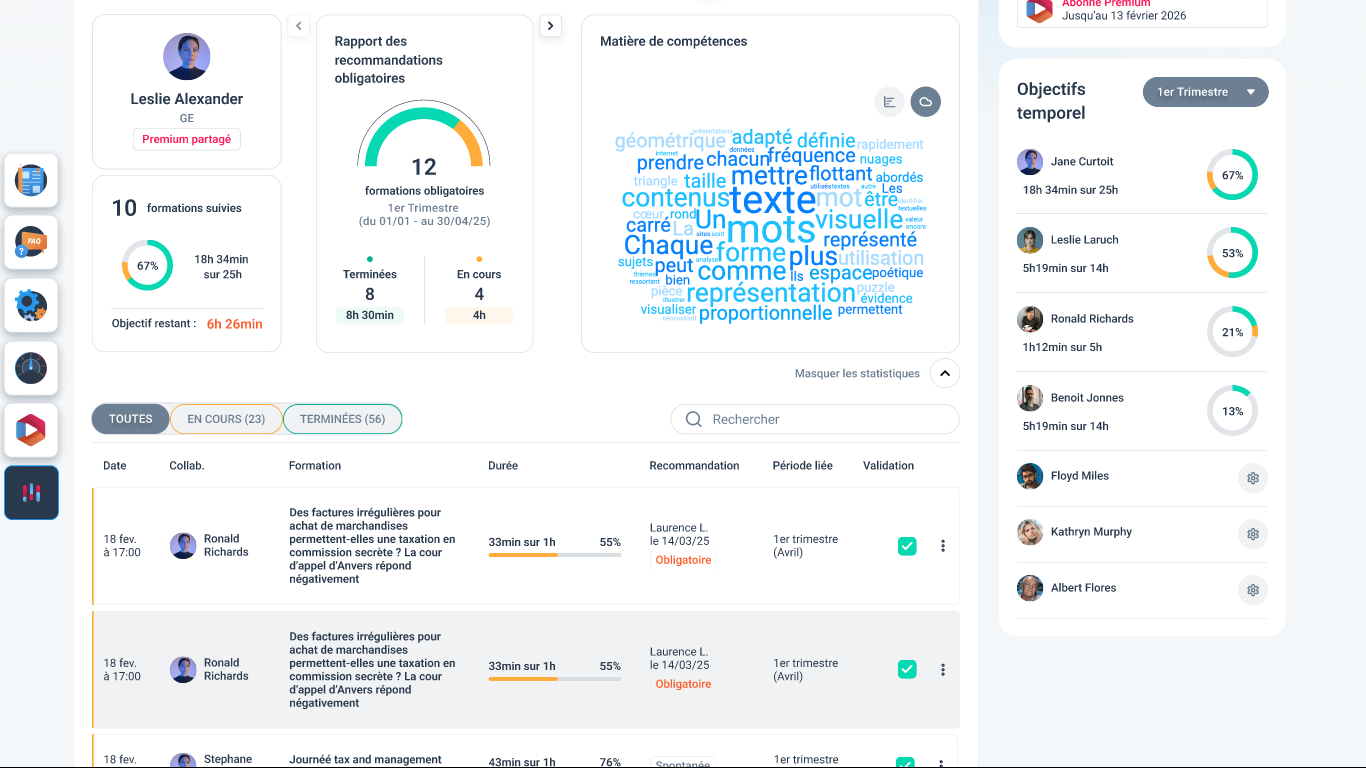
\includegraphics[width=\textwidth]{realisation/userwithmot.png}
    \caption{Interface des recommandations}
    \label{fig:interface_recommandations}
\end{figure}

L'interface des recommandations offre :
\begin{itemize}
    \item \textbf{Profil utilisateur} : Affichage des informations personnelles et du statut Premium
    \item \textbf{Rapport des recommandations obligatoires} : Visualisation graphique des formations obligatoires avec indicateurs de progression
    \item \textbf{Matière de compétences} : Nuage de mots interactif présentant les domaines de compétences
    \item \textbf{Historique des formations} : Liste détaillée des formations suivies et à suivre
\end{itemize}

\subsection{Interface de création d'objectifs}
Cette interface permet aux gestionnaires de définir et configurer les objectifs de formation pour leurs équipes.

\begin{figure}[H]
    \centering
    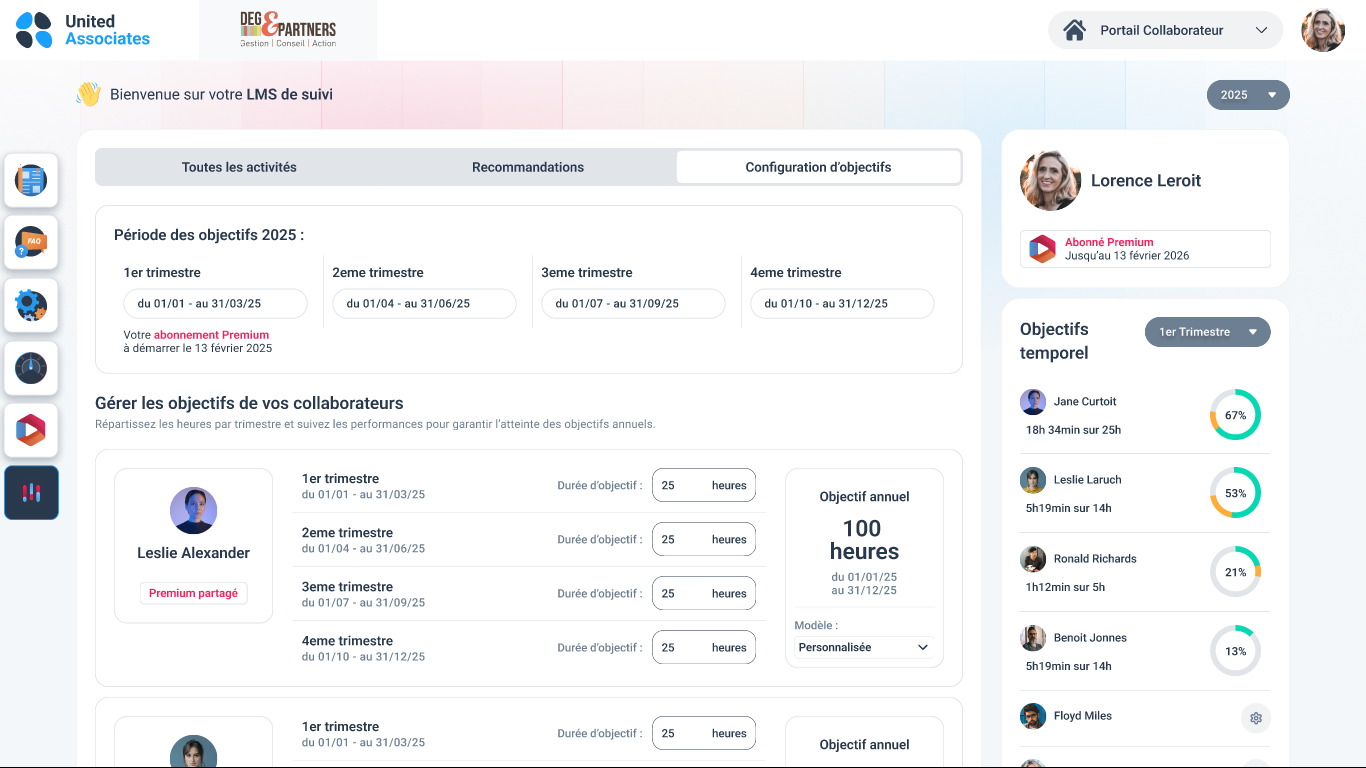
\includegraphics[width=\textwidth]{realisation/goal.png}
    \caption{Interface de création d'objectifs}
    \label{fig:creation_objectifs}
\end{figure}

Les fonctionnalités incluent :
\begin{itemize}
    \item \textbf{Création de modèles d'objectifs} : Définition de titres et paramètres personnalisés
    \item \textbf{Gestion par trimestre} : Répartition des objectifs sur l'année avec durées spécifiques
    \item \textbf{Objectifs annuels} : Configuration d'objectifs globaux avec suivi temporel
\end{itemize}

\subsection{Interface de configuration des objectifs collaborateurs}
Cette interface permet une gestion détaillée des objectifs individuels des collaborateurs.

\begin{figure}[H]
    \centering
    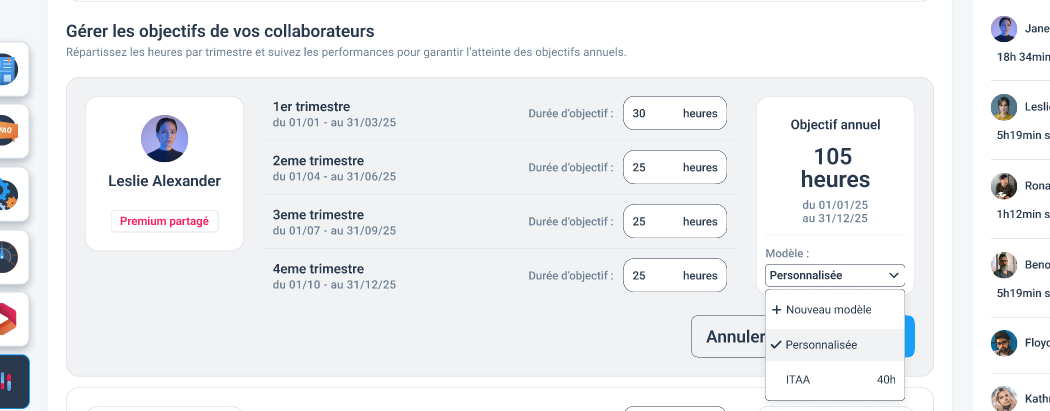
\includegraphics[width=\textwidth]{realisation/model.png}
    \caption{Interface de configuration des objectifs}
    \label{fig:config_objectifs}
\end{figure}

Elle comprend :
\begin{itemize}
    \item \textbf{Gestion par période} : Visualisation des objectifs par trimestre avec dates précises
    \item \textbf{Objectifs personnalisés} : Configuration d'heures de formation par collaborateur
    \item \textbf{Suivi des performances} : Affichage des objectifs annuels et du progrès réalisé
\end{itemize}

\subsection{Interface de recommandation de formations}
Cette interface facilite la recherche et l'assignation de formations aux collaborateurs.

\begin{figure}[H]
    \centering
    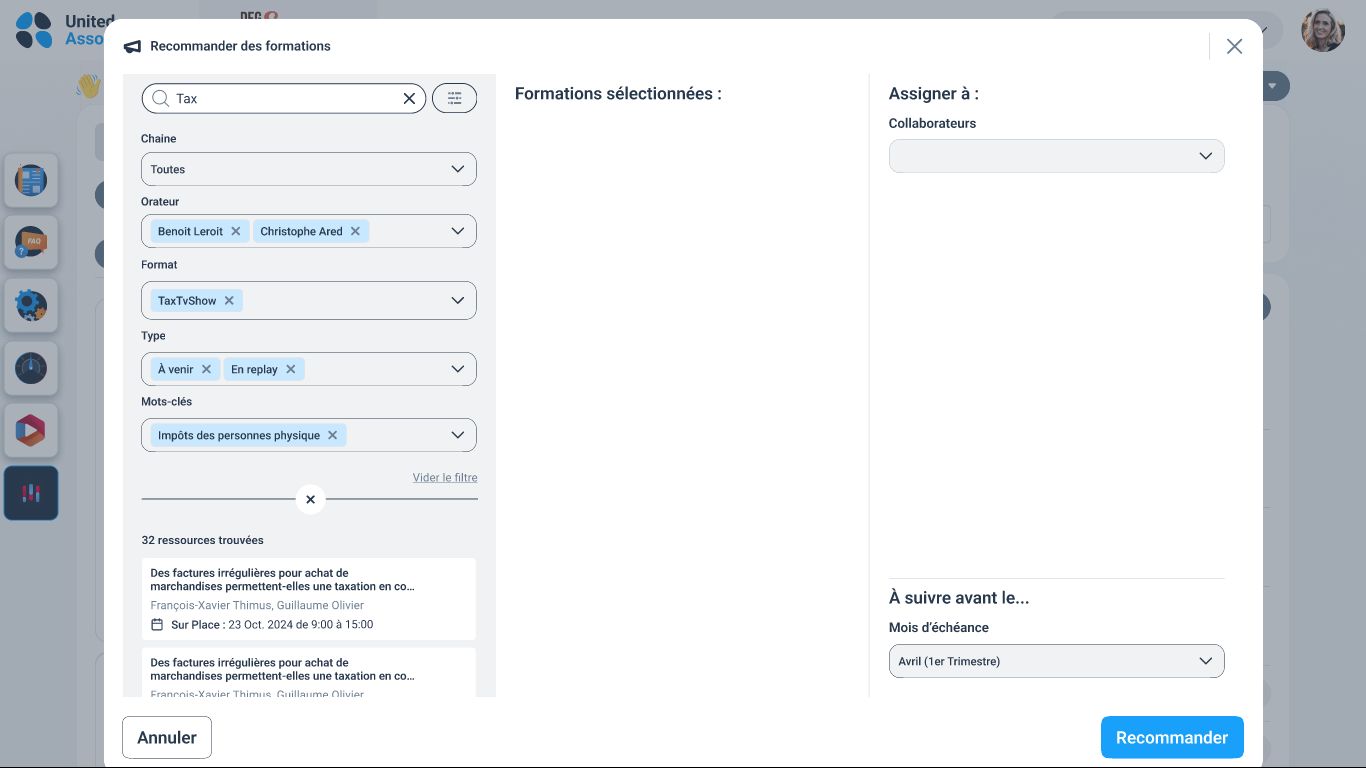
\includegraphics[width=\textwidth]{realisation/cherch.png}
    \caption{Interface de recherche de formations}
    \label{fig:recherche_formations}
\end{figure}

Les fonctionnalités principales sont :
\begin{itemize}
    \item \textbf{Moteur de recherche} : Recherche par mots-clés dans le catalogue de formations
    \item \textbf{Filtrage avancé} : Sélection de formations spécifiques par critères
    \item \textbf{Assignation multiple} : Possibilité d'assigner des formations à plusieurs collaborateurs
    \item \textbf{Planification} : Configuration des échéances et modalités de formation
\end{itemize}

\subsection{Interface de sélection et assignation}
Cette interface permet une gestion fine de l'assignation des formations aux équipes.

\begin{figure}[H]
    \centering
    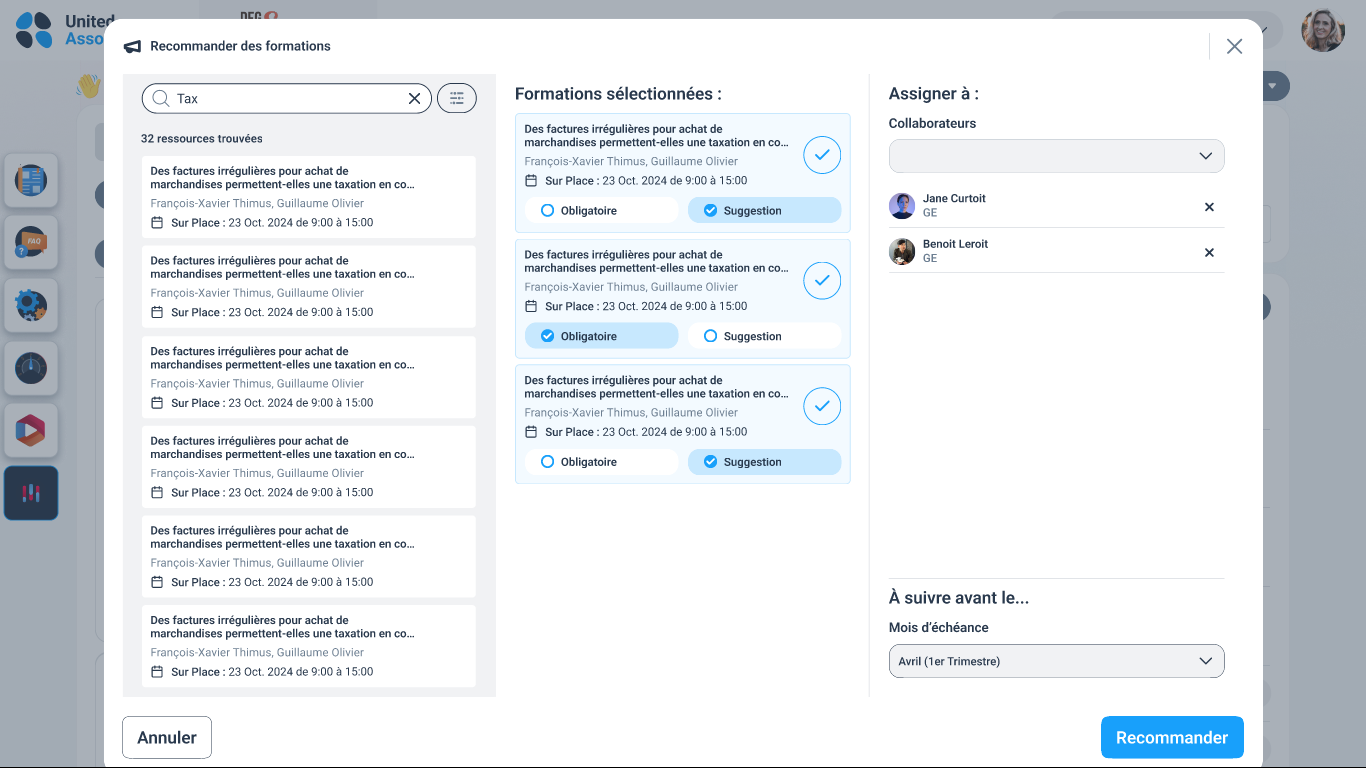
\includegraphics[width=\textwidth]{realisation/selection.png}
    \caption{Interface de sélection des formations}
    \label{fig:selection_formations}
\end{figure}

Elle offre :
\begin{itemize}
    \item \textbf{Sélection multiple} : Choix de plusieurs formations simultanément
    \item \textbf{Types de recommandations} : Distinction entre formations obligatoires et suggestions
    \item \textbf{Gestion des collaborateurs} : Assignation ciblée par collaborateur
    \item \textbf{Planification temporelle} : Configuration des dates d'échéance
\end{itemize}

\subsection{Interface de suivi des recommandations}
Cette interface présente le suivi des formations recommandées et leur statut d'avancement.

\begin{figure}[H]
    \centering
    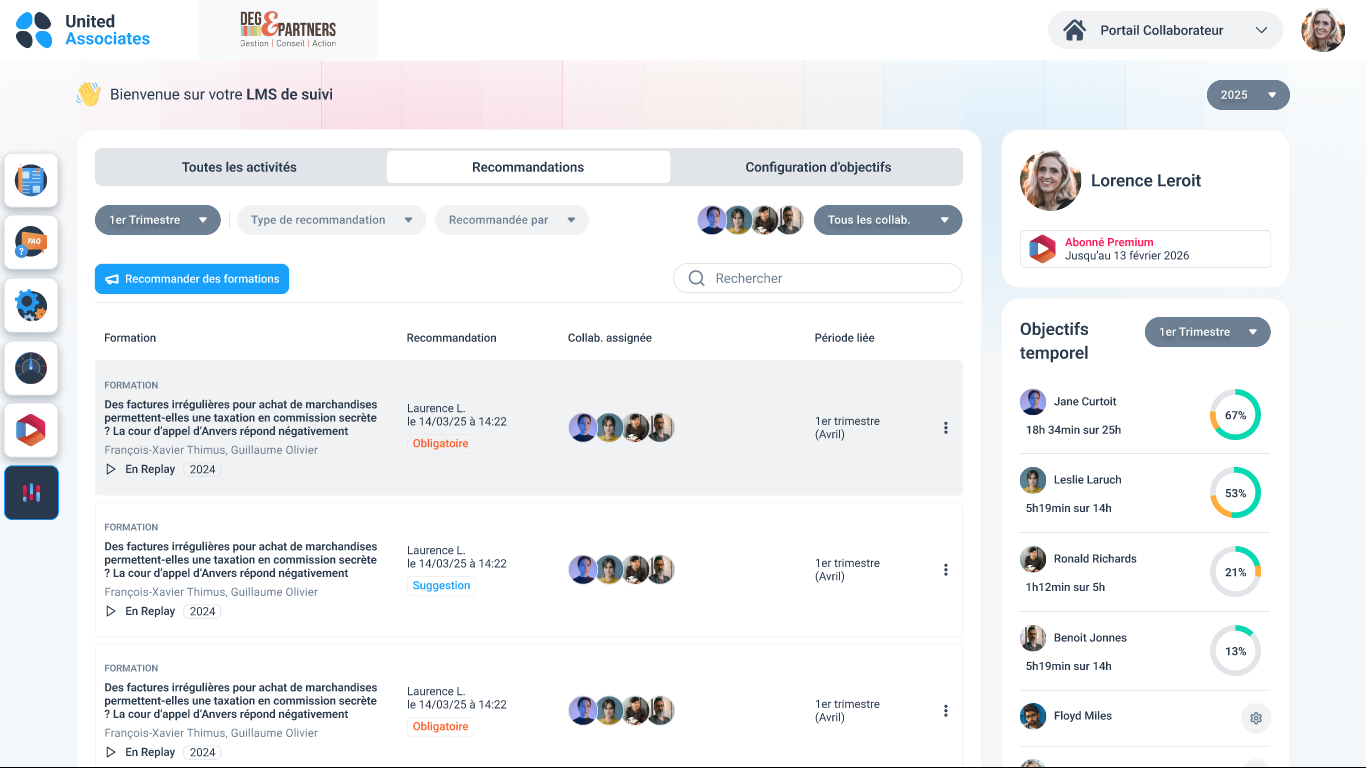
\includegraphics[width=\textwidth]{realisation/recomendation.png}
    \caption{Interface de suivi des recommandations}
    \label{fig:suivi_recommandations}
\end{figure}

Les éléments clés comprennent :
\begin{itemize}
    \item \textbf{Tableau de suivi} : Vue d'ensemble des formations assignées
    \item \textbf{Statuts de recommandation} : Distinction entre obligations et suggestions
    \item \textbf{Suivi par collaborateur} : Visualisation des formations par équipe
    \item \textbf{Indicateurs de progression} : Suivi des échéances et de l'avancement
\end{itemize}

\section{Fonctionnalités transversales}

\subsection{Système de notification}
Le système intègre un mécanisme de notifications pour informer les utilisateurs des échéances, nouvelles formations et objectifs à atteindre.

\subsection{Tableaux de bord personnalisés}
Chaque utilisateur dispose d'un tableau de bord adapté à son rôle (collaborateur, gestionnaire, formateur) avec des métriques pertinentes.

\subsection{Système de reporting}
Des rapports détaillés permettent le suivi des performances individuelles et collectives, facilitant la prise de décision managériale.
\section{Planification et suivi du projet}

\subsection{Diagramme de Gantt réel}
Le diagramme de Gantt ci-dessous présente la planification réelle du projet de développement du LMS de United Associates, montrant les différentes phases de réalisation, les jalons importants et l'état d'avancement des tâches sur la période de février à juillet 2025.

\begin{figure}[H]
    \centering
    
\includegraphics[width=\textwidth]{gantt_reel.png}
    \caption{Diagramme de Gantt réel du projet LMS}
    \label{fig:gantt_reel}
\end{figure}
Ce diagramme illustre :
\begin{itemize}
    \item \textbf{Phases de développement} : Répartition temporelle des différentes étapes du projet
    \item \textbf{Jalons critiques} : Points de contrôle et livrables importants marqués par des losanges
    \item \textbf{Progression réelle} : Comparaison entre la planification initiale et l'avancement effectif
    \item \textbf{Tâches parallèles} : Identification des activités menées simultanément
    \item \textbf{Dépendances} : Relations entre les différentes tâches du projet
\end{itemize}

L'analyse de ce diagramme révèle que le projet a globalement respecté les échéances prévues, avec quelques ajustements mineurs dans la planification pour optimiser les ressources et la qualité des livrables.
\section{Conclusion}
Ce chapitre a présenté les principales interfaces LMS, illustrant la richesse fonctionnelle de la plateforme. L'ensemble des interfaces développées offre une expérience utilisateur complète, allant de la gestion des objectifs individuels au suivi global des formations, en passant par un système de recommandations personnalisées. Le diagramme de Gantt réel témoigne du respect de la planification et de la bonne gestion temporelle du projet. Cette architecture modulaire permet une adaptation flexible aux besoins spécifiques de chaque organisation tout en maintenant une cohérence ergonomique et fonctionnelle.

% Conclusion Générale et Perspectives
\chapter*{Conclusion Générale et Perspectives}
\addcontentsline{toc}{chapter}{Conclusion Générale et Perspectives}
\markboth{Conclusion Générale et Perspectives}{}

\section*{Conclusion Générale}

Ce projet de fin d'études, réalisé au sein de l'entreprise \textbf{TAMTAM International}, m'a permis de concevoir et de développer une application de gestion des webinaires destinée aux fiduciaires belges. Tout au long de ce stage, j'ai pu mettre en pratique les connaissances théoriques acquises durant ma formation en Master Ingénierie des Systèmes d'Information, tout en me confrontant aux réalités et aux exigences du monde professionnel.

Sur le plan technique, ce projet m'a permis de maîtriser un ensemble de technologies modernes et complémentaires : \textbf{Meteor.js} et \textbf{React.js} côté frontend, \textbf{Symfony} côté backend, ainsi que les bases de données \textbf{MongoDB} et \textbf{MySQL}. La mise en œuvre de la méthodologie \textbf{Agile Scrum} a favorisé une organisation rigoureuse du travail, une livraison itérative des fonctionnalités et une communication efficace au sein de l'équipe.

Les résultats obtenus sont satisfaisants : la solution développée permet de gérer efficacement les webinaires, d'automatiser plusieurs opérations clés — telles que l'envoi de certificats de participation et la gestion des sondages — et d'améliorer sensiblement l'expérience des utilisateurs. Les fonctionnalités livrées répondent aux besoins exprimés par les parties prenantes et s'intègrent harmonieusement dans l'écosystème existant de la plateforme TAMTAM.

Sur le plan personnel, cette expérience a été particulièrement enrichissante. Elle m'a permis de développer mon autonomie, mon sens des responsabilités et ma capacité à travailler en équipe dans un contexte professionnel international. Elle m'a également conforté dans mon choix de carrière en ingénierie des systèmes d'information.

\section*{Perspectives}

Bien que les objectifs initiaux aient été atteints, plusieurs pistes d'amélioration et d'évolution méritent d'être envisagées pour les versions futures de la plateforme :

\begin{itemize}
    \item \textbf{Amélioration des performances} : optimisation des requêtes et mise en cache pour gérer un plus grand nombre d'utilisateurs simultanés lors des webinaires en direct.

    \item \textbf{Extension des fonctionnalités mobiles} : développement d'une application mobile native (iOS/Android) pour offrir une expérience utilisateur optimale sur smartphones et tablettes.

    \item \textbf{Intelligence artificielle} : intégration de mécanismes de recommandation basés sur le comportement des utilisateurs pour suggérer des webinaires pertinents et personnaliser le contenu.

    \item \textbf{Accessibilité} : mise en conformité avec les standards d'accessibilité WCAG 2.1 afin de rendre la plateforme utilisable par des personnes en situation de handicap.

    \item \textbf{Internationalisation} : extension du support multilingue pour couvrir de nouveaux marchés au-delà de la Belgique francophone.

    \item \textbf{Analytique avancée} : mise en place de tableaux de bord analytiques permettant aux organisateurs de suivre en temps réel les indicateurs clés de performance de leurs webinaires.
\end{itemize}

Ces perspectives ouvrent des horizons prometteurs pour la plateforme TAMTAM et témoignent du potentiel d'évolution d'une solution déjà robuste et fonctionnelle.


% Références bibliographiques
\cleardoublepage
\phantomsection
\section*{Références bibliographiques}
\addcontentsline{toc}{section}{Références bibliographiques}

\begin{enumerate}

\item K.~Schwaber and J.~Sutherland, \textit{The Scrum Guide: The Definitive Guide to Scrum --- The Rules of the Game}, Scrum.org, Nov. 2020. [En ligne]. Disponible~: \url{https://scrumguides.org/scrum-guide.html}

\item G.~Booch, J.~Rumbaugh, and I.~Jacobson, \textit{The Unified Modeling Language User Guide}, 2nd~ed. Boston, MA, USA: Addison-Wesley, 2005.

\item TAMTAM International, \textit{Documentation interne de la plateforme TamTam Webinar / OffCourse}, rapport interne, Marrakech, Maroc, 2025.

\item Meteor Development Group, \textit{Meteor.js --- Full-Stack JavaScript Framework, Official Documentation}, version~2.x, 2024. [En ligne]. Disponible~: \url{https://docs.meteor.com/}

\item OpenJS Foundation, \textit{Node.js Official Documentation}, version~20 LTS, 2024. [En ligne]. Disponible~: \url{https://nodejs.org/en/docs/}

\item SensioLabs, \textit{Symfony Framework --- Official Documentation}, version~6.x, 2024. [En ligne]. Disponible~: \url{https://symfony.com/doc}

\item Meta Platforms Inc., \textit{React --- A JavaScript Library for Building User Interfaces, Official Documentation}, 2024. [En ligne]. Disponible~: \url{https://react.dev/}

\item Vercel Inc., \textit{Next.js --- The React Framework, Official Documentation}, version~14, 2024. [En ligne]. Disponible~: \url{https://nextjs.org/docs}

\item MongoDB Inc., \textit{MongoDB Manual --- Official Documentation}, version~7.0, 2024. [En ligne]. Disponible~: \url{https://www.mongodb.com/docs/manual/}

\item Microsoft Corporation, \textit{TypeScript --- JavaScript With Syntax For Types, Official Documentation}, version~5.x, 2024. [En ligne]. Disponible~: \url{https://www.typescriptlang.org/docs/}

\end{enumerate}

\end{document}